% Task C22
% Source volume: lower
% Physical scan pages: 251--290
% Printed book pages: 239--278
% Transcribe only source content; omit running headers, footers, and printed page numbers.
\chapter{重积分}

从本章开始进入多元函数积分学。这一章主要介绍重积分（含广义重积分）及其在几何、物理和不等式证明中的应用。

本章分为六节：§22.1 和 §22.2 分别讲述二重积分的概念与计算；§22.3 讨论三重积分与 $n$ 重积分；§22.4 是广义重积分；§22.5 是重积分在几何、物理以及不等式证明中的应用；最后一节是学习要点和两组参考题。

\section{二重积分的概念}

\subsection{二重积分的定义}

在形式上与一元函数的定积分类似，可对二元函数的重积分定义如下：

设二元函数 $f$ 在可求面积的有界区域 $D\subset\RR^2$ 上定义，如果存在极限
\begin{equation}
  \lim_{\norm{T}\to0}\sum f(\xi_i,\eta_i)\Delta\sigma_i,
  \tag{22.1}
  \label{eq:22.1}
\end{equation}
则称 $f$ 在 $D$ 上可积，并称其极限值为 $f$ 在 $D$ 上的二重积分，记为
\[
  \iint_D f(x,y)\,\dd x\,\dd y.
\]
在 (22.1) 中，$T$ 是 $D$ 的任一分划，$\norm{T}$ 为子区域的最大直径，$\sigma_i$ 为第 $i$ 个可求面积的子区域，$\Delta\sigma_i$ 为 $\sigma_i$ 的面积，$(\xi_i,\eta_i)$ 是 $\sigma_i$ 中任一点。

在上述定义中有两点是要加以特别说明的。第一，怎样定义可求面积的区域？如何定义分划 $T$ 使子区域均可求面积？第二，为什么要用子区域的最大直径来刻画分划的模 $\norm{T}$？对于第二点比较容易理解。因为如果用子区域的最大面积来刻画分划的模的话，即使子区域的面积很小，但在同一子区域的点可能相距很远。因此“以直代曲”就不可能在一个小范围内实现。对于第一点，现行教科书中有两类解决的方案。在一些教科书上是先考虑在矩形区域上的二重积分（见 [36, 8] 等），因而分划 $T$ 自然是用直线网来实现。把 $D$ 分成有限个小矩形，(22.1) 式的含义也是很清楚的。对于一般的区域 $D$ 上函数 $f$ 的二重积分，通过 $f$ 对 $D$ 的特征函数
\[
  f_D(x,y)=
  \begin{cases}
    f(x,y), & \text{当 }(x,y)\in D\text{ 时},\\
    0, & \text{其他}
  \end{cases}
\]
来过渡。第二类方案（见 [24, 11, 28, 9] 等）是先定义平面区域的面积。一个平面区域 $D$ 可求面积是指 $\forall\varepsilon>0$，存在有限个矩形组成的多边形 $\Sigma_1,\Sigma_2$，使 $\Sigma_1\subset D\subset\Sigma_2$，且使得 $\Sigma_2$ 的面积减 $\Sigma_1$ 的面积 $<\varepsilon$。又如果一条曲线可用有限个面积任意小的矩形覆盖，则称这条曲线是零面积的。平面区域 $D$ 可求面积的充分必要条件为边界 $\partial D$ 是零面积的。因此分划 $T$ 是用有限条零面积的曲线网来实现的。读者可参考相应的教科书对这个定义作进一步的理解。

\subsection{可积函数类}

先引进平面 $\RR^2$ 内的零测度集（参见上册 304 页关于一维零测度集的定义）。设 $S$ 是 $\RR^2$ 内的一个点集，如果 $\forall\varepsilon>0$，存在可列个矩形 $\Delta_1,\Delta_2,\ldots,\Delta_n,\ldots$，使得
\begin{enumerate}[label=(\arabic*)]
  \item $\displaystyle\bigcup_{n=1}^{\infty}\Delta_n\supset S$，即矩形集 $\{\Delta_n\}$ 覆盖了 $S$；
  \item $\displaystyle\sum_{n=1}^{\infty}\abs{\Delta_n}<\varepsilon$，其中 $\abs{\Delta_n}$ 为 $\Delta_n$ 的面积，
\end{enumerate}
则称 $S$ 是 $\RR^2$ 内的一个零测度集。注意零面积集必是零测度集，但零测度集不一定是零面积集。例如 $\RR^2$ 中有理点全体组成的集是零测度集，但不是零面积集。

与一元函数的定积分类似，我们有如下的可积充分必要条件（参见上册 304 页的 Lebesgue 定理）。

\begin{xproposition}[22.1.1]
设 $D$ 为可求面积的有界闭区域，$f$ 是定义在 $D$ 上的有界函数，则 $f$ 在 $D$ 上可积的充分必要条件是 $f$ 在 $D$ 上的所有不连续点的集合是零测度集。
\end{xproposition}

命题 22.1.1 的证明可参见 [28] 等。由命题 22.1.1 立得：$D$ 上的连续函数是可积的；只有至多可列个不连续点的有界函数是可积的；甚至若有界函数 $f$ 的所有不连续点组成 $D$ 的有限条零测度的曲线，则 $f$ 也是可积的。

二重积分的性质与一元函数的定积分完全类似，这里不再重复。如不作特殊申明，以下均假设 $D$ 为可求面积的有界闭区域。

\begin{xexample}[22.1.1]
设曲线 $l\colon x=\varphi(t),y=\psi(t),\alpha\le t\le\beta$，其中 $\varphi,\psi$ 连续，且至少其中之一有连续导数，则曲线 $l$ 的面积为零。
\end{xexample}
\begin{xproof}
不妨设 $\varphi(t)$ 在闭区间 $[\alpha,\beta]$ 上连续，$\psi(t)$ 有连续导函数。$\forall\varepsilon>0$，可作分割
\[
  \alpha=t_0<t_1<\cdots<t_n=\beta,
\]
使当 $s,t\in[t_{j-1},t_j]$，$j=1,2,\ldots,n$ 时有
\[
  \abs{\varphi(s)-\varphi(t)}<\varepsilon.
\]
令
\[
  a_j=\min_{t_{j-1}\le t\le t_j}\{\varphi(t)\},\qquad
  b_j=\max_{t_{j-1}\le t\le t_j}\{\varphi(t)\},
\]
则有
\[
  b_j-a_j\le\varepsilon,\qquad j=1,2,\ldots,n.
\]
又令
\[
  c_j=\min_{t_{j-1}\le t\le t_j}\{\psi(t)\},\qquad
  d_j=\max_{t_{j-1}\le t\le t_j}\{\psi(t)\},\qquad
  I_j=[a_j,b_j]\times[c_j,d_j],
\]
于是当 $t\in[t_{j-1},t_j]$ 时 $(\varphi(t),\psi(t))\in I_j$，故曲线 $l\subset\bigcup_{j=1}^n I_j$。由于 $\psi'(t)$ 在闭区间 $[\alpha,\beta]$ 上连续，所以
\[
  \abs{\psi'(t)}\le M,\qquad \alpha\le t\le\beta.
\]
由微分中值定理得
\[
  d_j-c_j\le M(t_j-t_{j-1}),\qquad j=1,2,\ldots,n.
\]
因而
\[
  \sum_{j=1}^n\abs{I_j}
  \le\sum_{j=1}^n\varepsilon M(t_j-t_{j-1})
  =\varepsilon M(\beta-\alpha),
\]
其中 $\abs{I_j}$ 表示矩形 $I_j$ 的面积。因为 $\varepsilon$ 是任意的，故曲线 $l$ 的面积为零。
\end{xproof}

\begin{xremark}
在后面我们将要遇到的大多数区域（如 $x$ 型区域、$y$ 型区域）都是由有限条满足上例条件的曲线段所围成的，因此这样的区域都是可求面积的。
\end{xremark}

\begin{xexample}[22.1.2]
设有界非负函数 $f$ 在区域 $D$ 上可积。证明：积分
\begin{equation}
  \iint_D f(x,y)\,\dd x\,\dd y=0
  \tag{22.2}
  \label{eq:22.2}
\end{equation}
的充分必要条件是 $f$ 在其连续点处的值均为零（参见上册 333 页题 9）。
\end{xexample}
\begin{xproof}
先证必要性。用反证法：若不然，存在 $p_0(x_0,y_0)\in D$，$f$ 在点 $p_0$ 连续，且 $f(x_0,y_0)>0$。由连续函数的局部保号性定理知存在 $\delta>0$，使得
\[
  f(x,y)>\frac12f(x_0,y_0),\qquad \forall(x,y)\in O_\delta(p_0)\subset D.
\]
于是
\[
  \iint_D f(x,y)\,\dd x\,\dd y
  \ge \iint_{O_\delta(p_0)}\frac12f(x_0,y_0)\,\dd x\,\dd y
  =\frac{\pi}{2}\delta^2f(x_0,y_0)>0,
\]
与 (22.2) 矛盾。

再证充分性。设 $f(x,y)$ 在其连续点处的函数值为 0。对任意分划 $T$ 中可求面积的小区域 $\sigma_i$，如 $\Delta\sigma_i>0$，则 $\sigma_i$ 不是零测度集。由可积充分必要条件知在每一个 $\sigma_i$ 内至少有 $f$ 的一个连续点，记之为 $(\xi_i,\eta_i)$，作和数 $\sum_{i=1}^n f(\xi_i,\eta_i)\Delta\sigma_i$，则
\[
  \sum_{i=1}^n f(\xi_i,\eta_i)\Delta\sigma_i=0.
\]
于是
\[
  \iint_D f(x,y)\,\dd x\,\dd y
  =\lim_{\norm{T}\to0}\sum_{i=1}^n f(\xi_i,\eta_i)\Delta\sigma_i=0.
\]
\end{xproof}

\begin{xexample}[22.1.3]
设 $D_R$ 是由 $x=R,y=0,y=\frac{2}{R}x-1$ 围成，求
\[
  \lim_{R\to+\infty}\iint_{D_R}\ee^{-x}\arctan\frac{y}{x}\,\dd x\,\dd y.
\]
\end{xexample}
\begin{xsolution}
在图 22.1 中作出了区域 $D_R$ 的图形。
\begin{center}
  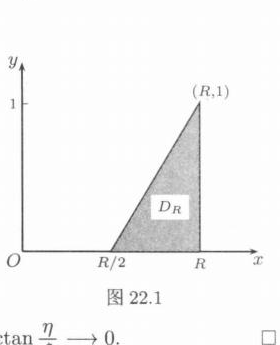
\includegraphics[width=.36\linewidth]{figures/lower/ch22/fig-22-1.png}
\end{center}
由于函数 $\ee^{-x}\arctan\frac{y}{x}$ 在 $D_R$ 上连续，由积分中值定理，存在 $(\xi,\eta)\in D_R$，使得
\[
  \iint_{D_R}\ee^{-x}\arctan\frac{y}{x}\,\dd x\,\dd y
  =\ee^{-\xi}\arctan\frac{\eta}{\xi}\cdot\abs{D_R}
  =\frac{R}{4}\ee^{-\xi}\arctan\frac{\eta}{\xi},
\]
其中 $\frac{R}{2}\le\xi\le R,0\le\eta\le1$。于是当 $R\to+\infty$ 时
\[
  \abs*{\iint_{D_R}\ee^{-x}\arctan\frac{y}{x}\,\dd x\,\dd y}
  \le\frac{R}{4}\ee^{-R/2}\arctan\frac{\eta}{\xi}\to0.
\]
\end{xsolution}

\subsection{思考题}

\begin{xthought}[1]
设 $f(x,y),g(x,y)$ 在 $D$ 上可积，证明：$f(x,y)\cdot g(x,y)$ 也在 $D$ 上可积。设 $f(x,y)$ 在 $D$ 上可积，且 $f(x,y)\ne0$，证明：$\frac1{f(x,y)}$ 也在 $D$ 上可积。
\end{xthought}
\begin{xsolution}
若 $f,g$ 在 $D$ 上可积，则二者均有界。由可积判别准则，$f,g$ 的不连续点集分别为零测度集 $E_f,E_g$。在 $D\setminus(E_f\cup E_g)$ 上，$f,g$ 都连续，因此 $fg$ 连续。故 $fg$ 的不连续点集包含于 $E_f\cup E_g$，仍为零测度集，所以 $fg$ 在 $D$ 上可积。

题目中关于倒数的断言按原条件并不成立。取 $D=[0,1]\times[0,1]$，定义
\[
  f(x,y)=
  \begin{cases}
    x,&x>0,\\
    1,&x=0.
  \end{cases}
\]
$f$ 有界，且仅在直线 $x=0$ 上不连续，所以在 $D$ 上可积；又处处有 $f\ne0$。但是
\[
  \frac1{f(x,y)}=
  \begin{cases}
    1/x,&x>0,\\
    1,&x=0
  \end{cases}
\]
在 $D$ 上无界，因而不是通常意义下的 Riemann 可积函数。

若补充条件 $\abs{f(x,y)}\ge m>0$，则 $1/f$ 有界，而且在 $f$ 的每个连续点处连续，故其不连续点集仍包含于 $f$ 的不连续点集，从而 $1/f$ 可积。
\end{xsolution}


\begin{xthought}[2]
设 $u=u(x,y)$ 在 $D$ 上可积，$f(u)$ 是 $u$ 的连续函数，证明：$f(u(x,y))$ 在 $D$ 上可积。如果 $f(u)$ 仅仅是 $u$ 的可积函数，$f(u(x,y))$ 是否一定在 $D$ 上可积？
\end{xthought}
\begin{xsolution}
设 $u(D)\subset[m,M]$。因为 $u$ 可积，所以 $u$ 有界，且其不连续点集 $E$ 为零测度集。若 $f$ 在 $[m,M]$ 上连续，则在 $D\setminus E$ 的每一点 $(x_0,y_0)$，$u$ 连续，复合函数连续性给出
\[
  f(u(x,y))\longrightarrow f(u(x_0,y_0)).
\]
因此 $f\circ u$ 的不连续点集包含于 $E$。又 $f$ 在紧区间上有界，所以 $f(u(x,y))$ 有界。由可积判别准则，$f(u(x,y))$ 在 $D$ 上可积。

若 $f$ 仅仅可积，结论不成立。取 $D=[0,1]^2$，令 Thomae 函数
\[
  T(x)=
  \begin{cases}
    1/q,&x=p/q\text{ 为既约有理数},\\
    0,&x\text{ 为无理数},
  \end{cases}
\]
并令 $u(x,y)=T(x)$。$u$ 的不连续点集为 $\QQ\cap[0,1]$ 与 $[0,1]$ 的直积，是零测度集，所以 $u$ 可积。再定义
\[
  f(t)=
  \begin{cases}
    1,&t=0,\\
    0,&t\ne0.
  \end{cases}
\]
$f$ 在 $[0,1]$ 上只有 $t=0$ 一个不连续点，故可积。然而
\[
  f(u(x,y))=
  \begin{cases}
    1,&x\text{ 为无理数},\\
    0,&x\text{ 为有理数},
  \end{cases}
\]
在 $D$ 的每一点都不连续，因而不可积。
\end{xsolution}


\begin{xthought}[3]
设 $f(x,y),g(x,y)$ 在 $D$ 上有界，且在 $D$ 上除了一个零面积集外处处相等。证明：$f(x,y)$ 与 $g(x,y)$ 在 $D$ 上有相同的可积性，可积时有相同的积分值。如果 $f(x,y)$ 与 $g(x,y)$ 在 $D$ 上除了一个零测度集外处处相等，情况又如何？
\end{xthought}
\begin{xsolution}
先设 $f=g$ 除了一个零面积集 $E$ 外处处成立，并令 $h=f-g$。由于 $f,g$ 有界，存在 $M>0$ 使 $\abs{h}\le M$。对任意 $\varepsilon>0$，可用有限个矩形覆盖 $E$，使这些矩形的总面积小于 $\varepsilon$。在覆盖之外 $h=0$，所以对应任一足够细的分划，$h$ 的上下和之差只来自这些矩形，且不超过 $2M\varepsilon$。由 $\varepsilon$ 的任意性，$h$ 可积且
\[
  \iint_D h(x,y)\,\dd x\,\dd y=0.
\]
于是 $f$ 与 $g$ 有相同的可积性；可积时
\[
  \iint_Df\,\dd x\,\dd y=\iint_Dg\,\dd x\,\dd y.
\]

若把“零面积集”换成一般的“零测度集”，结论不再成立。取 $D=[0,1]^2$，令 $f\equiv0$，而
\[
  g(x,y)=\mathbf 1_{(\QQ\cap[0,1])^2}(x,y).
\]
两函数仅在可列集 $(\QQ\cap[0,1])^2$ 上不同，这个集合是零测度集；但 $g$ 在每一点附近同时取得 $0$ 和 $1$，故处处不连续，不可积，而 $f$ 可积。
\end{xsolution}


\begin{xthought}[4]
如果 $f(x,y)$ 在 $\overline D\subset D$ 上有界可积，且 $D\setminus\overline D$ 为零面积集。我们可以认为 $f(x,y)$ 在 $D$ 上可积，且其积分值就取 $f(x,y)$ 在 $\overline D$ 上的积分值。讨论：
  \begin{enumerate}[label=(\arabic*)]
    \item $\displaystyle f(x,y)=\sin\frac1{(x^2-1)^2+(y^2-1)^2}$ 在 $[-1,1]\times[-1,1]$ 上；
    \item $\displaystyle f(x,y)=\arctan\frac1{y-x^2}$ 在 $[0,1]\times[0,1]$ 上
  \end{enumerate}
  的可积性。
\end{xthought}
\begin{xsolution}
\begin{enumerate}[label=(\arabic*)]
  \item 函数
  \[
    f(x,y)=\sin\frac1{(x^2-1)^2+(y^2-1)^2}
  \]
  在正方形 $[-1,1]^2$ 内有界，只有四个角点 $(\pm1,\pm1)$ 是奇点。在这些点任意补定义函数值后，所得函数的不连续点集至多为这四点，因而是零测度集。故函数在 $[-1,1]^2$ 上可积；对原函数按题目所述约定，其积分就是去掉四个角点后的积分。

  \item 函数
  \[
    f(x,y)=\arctan\frac1{y-x^2}
  \]
  在 $[0,1]^2$ 上有界。除抛物线弧 $y=x^2$ 外处处连续，而该曲线面积为零。在曲线上任意补定义后，不连续点集包含于这条零面积曲线，故函数可积。于是按题目约定，原函数在 $[0,1]^2$ 上可积。
\end{enumerate}
\end{xsolution}


\subsection{练习题}

\begin{xexercise}[1]
设 $f(x,y),g(x,y)$ 都是 $D$ 上的可积函数，证明：
  \[
    h(x,y)=\max\{f(x,y),g(x,y)\}
  \]
  也是 $D$ 上的可积函数。
\end{xexercise}
\begin{xsolution}
由
\[
  \max\{f,g\}=\frac12\bigl(f+g+\abs{f-g}\bigr)
\]
即可。$f-g$ 可积；若 $u$ 可积，则 $\abs{u}$ 的不连续点只能出现在 $u$ 的不连续点处，因此 $\abs{u}$ 也可积。于是 $\abs{f-g}$ 可积，从而 $h=\max\{f,g\}$ 可积。
\end{xsolution}


\begin{xexercise}[2]
设 $f(x,y)$ 在点 $p_0(x_0,y_0)$ 的某邻域中连续，求
  \[
    \lim_{\rho\to0}\frac1{\pi\rho^2}
    \iint_{(x-x_0)^2+(y-y_0)^2\le\rho^2}f(x,y)\,\dd x\,\dd y.
  \]
\end{xexercise}
\begin{xsolution}
记 $B_\rho(p_0)=\{(x,y)\mid(x-x_0)^2+(y-y_0)^2\le\rho^2\}$。由 $f$ 在 $p_0$ 连续，对任意 $\varepsilon>0$，存在 $\delta>0$，当 $0<\rho<\delta$ 且 $(x,y)\in B_\rho(p_0)$ 时有
\[
  \abs{f(x,y)-f(x_0,y_0)}<\varepsilon.
\]
因此
\begin{align*}
 &\abs*{\frac1{\pi\rho^2}\iint_{B_\rho(p_0)}f(x,y)\,\dd x\,\dd y-f(x_0,y_0)}\\
 &\qquad\le\frac1{\pi\rho^2}\iint_{B_\rho(p_0)}\abs{f(x,y)-f(x_0,y_0)}\,\dd x\,\dd y<\varepsilon.
\end{align*}
故极限为
\[
  \boxed{f(x_0,y_0)}.
\]
\end{xsolution}


\begin{xexercise}[3]
证明：
  \[
    \iint_{\abs{x}+\abs{y}\le1} f(x+y)\,\dd x\,\dd y
    =\int_{-1}^1 f(u)\,\dd u.
  \]
\end{xexercise}
\begin{xsolution}
作线性变换
\[
  u=x+y,\qquad v=x-y,
\]
则
\[
  x=\frac{u+v}{2},\qquad y=\frac{u-v}{2},\qquad
  \abs*{\frac{\partial(x,y)}{\partial(u,v)}}=\frac12.
\]
并且
\[
  \abs{x}+\abs{y}=\max\{\abs{u},\abs{v}\},
\]
故菱形 $\abs{x}+\abs{y}\le1$ 被变成正方形 $-1\le u,v\le1$。于是
\begin{align*}
  \iint_{\abs{x}+\abs{y}\le1}f(x+y)\,\dd x\,\dd y
  &=\frac12\int_{-1}^1\int_{-1}^1 f(u)\,\dd v\,\dd u\\
  &=\int_{-1}^1f(u)\,\dd u.
\end{align*}
\end{xsolution}


\begin{xexercise}[4]
证明：
  \[
    \iint_D f(xy)\,\dd x\,\dd y=\ln2\int_1^2 f(u)\,\dd u,
  \]
  其中 $D$ 为 $xy=1,xy=2,y=x,y=4x$ 在第一象限所围成的区域。
\end{xexercise}
\begin{xsolution}
在第一象限作变换
\[
  u=xy,\qquad v=\frac yx.
\]
区域的四条边分别变为 $u=1,u=2,v=1,v=4$。由
\[
  x=\sqrt{\frac uv},\qquad y=\sqrt{uv},
\]
得
\[
  \abs*{\frac{\partial(x,y)}{\partial(u,v)}}=\frac1{2v}.
\]
故
\begin{align*}
  \iint_Df(xy)\,\dd x\,\dd y
  &=\int_1^2\int_1^4 f(u)\frac1{2v}\,\dd v\,\dd u\\
  &=\frac12\ln4\int_1^2f(u)\,\dd u
  =\ln2\int_1^2f(u)\,\dd u.
\end{align*}
\end{xsolution}


\section{二重积分的计算}

\subsection{矩形区域上的二重积分}

矩形上的二重积分在一定条件下可以化为二次积分进行计算。

设 $f(x,y)$ 在矩形 $A=[a,b]\times[c,d]$ 上可积，且对每个固定的 $x\in[a,b]$，积分
\[
  \varphi(x)=\int_c^d f(x,y)\,\dd y
\]
存在，则 $\varphi(x)$ 在 $[a,b]$ 上可积，并且
\[
  \iint_A f(x,y)\,\dd x\,\dd y
  =\int_a^b\dd x\int_c^d f(x,y)\,\dd y.
\]

由此可以看出，若 $f(x,y)$ 在 $A$ 上连续，则两个二次积分是相等的（都等于二重积分），积分值与积分顺序无关。但积分顺序不同时，积分的难度可能相差很大。请看下面的例子。

\begin{xexample}[22.2.1]
设 $A=[0,1]\times[0,1]$，求
\[
  I=\iint_A\frac{y\,\dd x\,\dd y}{(1+x^2+y^2)^{3/2}}.
\]
\end{xexample}
\begin{xsolution}
先对 $y$ 后对 $x$ 积分，得到
\begin{align*}
  I&=\int_0^1\dd x\int_0^1\frac{y\,\dd y}{(1+x^2+y^2)^{3/2}}\\
   &=\int_0^1\left(\frac1{\sqrt{x^2+1}}-\frac1{\sqrt{x^2+2}}\right)\dd x
   =\ln\frac{2+\sqrt2}{1+\sqrt3}.
\end{align*}
先对 $x$ 后对 $y$ 积分，则得到
\begin{align*}
  I&=\int_0^1 y\,\dd y\int_0^1\frac{\dd x}{(1+x^2+y^2)^{3/2}}\\
   &=\int_0^1 y\left[\frac1{1+y^2}\cdot\frac{x}{(1+x^2+y^2)^{1/2}}\right]_{x=0}^{x=1}\dd y\\
   &=\int_0^1\frac{y\,\dd y}{(1+y^2)(2+y^2)^{1/2}}\qquad(\sqrt{2+y^2}=t)\\
   &=\int_{\sqrt2}^{\sqrt3}\frac{\dd t}{t^2-1}
   =\frac12\ln\left.\frac{t-1}{t+1}\right|_{\sqrt2}^{\sqrt3}\\
   &=\frac12\ln\frac{(\sqrt3-1)(\sqrt2+1)}{(\sqrt3+1)(\sqrt2-1)}
   =\frac12\ln\frac{2(\sqrt2+1)^2}{(\sqrt3+1)^2}
   =\ln\frac{2+\sqrt2}{1+\sqrt3}.
\end{align*}
\end{xsolution}

在 $f$ 不满足可积或累次可积的条件时，情况就比较复杂，请看下面反例。

\begin{xexample}[22.2.2]
设函数 $f$ 定义在 $A=[0,1]\times[0,1]$ 上，
\[
  f(x,y)=
  \begin{cases}
    1, & \text{当 }x\text{ 是无理数},\\
    2y, & \text{当 }x\text{ 是有理数},
  \end{cases}
\]
则
\begin{enumerate}[label=(\arabic*)]
  \item $f$ 在 $A$ 上不可积；
  \item $\displaystyle\int_0^1\dd x\int_0^1f(x,y)\,\dd y$ 存在，$\displaystyle\int_0^1\dd y\int_0^1f(x,y)\,\dd x$ 不存在。
\end{enumerate}
\end{xexample}
\begin{xproof}
(1) $\forall y\in[0,1],y\ne\frac12$，$f(x,y)$ 作为 $x$ 的函数在 $[0,1]$ 内处处不连续，所以 $f(x,y)$ 在 $A$ 上的 $y\ne\frac12$ 的每点处都不连续。于是 $f$ 在 $A$ 上不可积。

(2) 由于
\[
  \int_0^1f(x,y)\,\dd y=
  \begin{cases}
    \displaystyle\int_0^1\dd y=1, & \text{当 }x\text{ 为无理数},\\
    \displaystyle\int_0^1 2y\,\dd y=1, & \text{当 }x\text{ 为有理数},
  \end{cases}
\]
所以
\[
  \int_0^1\dd x\int_0^1f(x,y)\,\dd y=\int_0^1\dd x=1.
\]
另一方面，$\forall y\in[0,1],y\ne\frac12$，$f(x,y)$ 作为 $x$ 的一元函数，在 $[0,1]$ 内每一点处都不连续，于是 $\int_0^1f(x,y)\,\dd x$ 对每个 $y\ne\frac12$ 都不存在，从而
\[
  \int_0^1\dd y\int_0^1f(x,y)\,\dd x
\]
不存在。
\end{xproof}

类似地，也有二重积分存在，但两个二次积分不存在以及两个二次积分存在且相等，但二重积分不存在的例子。

\subsection{一般区域上的二重积分}

设 $f$ 是区域 $D$ 上的可积函数，又设 $D$ 可以表示为 $x$ 型区域：
\[
  D=\{(x,y)\mid y_1(x)\le y\le y_2(x),a\le x\le b\},
\]
其中 $y_1(x),y_2(x)$ 为 $x$ 的函数，且对每一个固定的 $x\in[a,b]$，积分
\[
  \varphi(x)=\int_{y_1(x)}^{y_2(x)}f(x,y)\,\dd y
\]
存在，则 $\varphi(x)$ 在 $[a,b]$ 上可积，且 $f$ 在 $D$ 上的二重积分可化为先对 $y$ 后对 $x$ 的积分
\[
  \iint_D f(x,y)\,\dd x\,\dd y
  =\int_a^b\dd x\int_{y_1(x)}^{y_2(x)}f(x,y)\,\dd y.
\]
同样地，如果区域 $D$ 可以表示为 $y$ 型区域
\[
  D=\{(x,y)\mid x_1(y)\le x\le x_2(y),c\le y\le d\},
\]
其中 $x_1(y),x_2(y)$ 为 $y$ 的函数，且对每一个固定的 $y\in[c,d]$，积分
\[
  \psi(y)=\int_{x_1(y)}^{x_2(y)}f(x,y)\,\dd x
\]
存在，则 $\psi(y)$ 在 $[c,d]$ 上可积，且有
\[
  \iint_D f(x,y)\,\dd x\,\dd y
  =\int_c^d\dd y\int_{x_1(y)}^{x_2(y)}f(x,y)\,\dd x.
\]

对于一般区域，如区域可分成若干个不相交的 $x$ 型区域和 $y$ 型区域的并，则可先分别计算这些区域上积分的值，然后通过积分的区域可加性求原积分的值。

在具体计算时，应根据积分区域和被积函数的情况，以方便计算为原则，权衡利弊，决定采用哪种积分区域的分解与积分顺序。画出积分区域的草图往往有助于做出正确的选择。

\begin{xexample}[22.2.3]
设区域
\[
  D=\{(x,y)\mid 2y\le x^2+y^2\le4y,x\ge0\}.
\]
分别将 $D$ 表示为 $x$ 型区域和 $y$ 型区域。
\end{xexample}
\begin{xsolution}
(1) 表示为 $x$ 型区域，$D$ 可分为三块（见图 22.2），其中
\[
  D_1=\begin{cases}
    0\le x\le1,\\
    2-\sqrt{4-x^2}\le y\le1-\sqrt{1-x^2},
  \end{cases}
\]
\[
  D_2=\begin{cases}
    0\le x\le1,\\
    1+\sqrt{1-x^2}\le y\le2+\sqrt{4-x^2},
  \end{cases}
\]
\[
  D_3=\begin{cases}
    1\le x\le2,\\
    2-\sqrt{4-x^2}\le y\le2+\sqrt{4-x^2}.
  \end{cases}
\]

(2) 表示为 $y$ 型区域，$D$ 可分为两块（见图 22.3），其中
\[
  E_1=\begin{cases}
    0\le y\le2,\\
    \sqrt{2y-y^2}\le x\le\sqrt{4y-y^2},
  \end{cases}
  \qquad
  E_2=\begin{cases}
    2\le y\le4,\\
    0\le x\le\sqrt{4y-y^2}.
  \end{cases}
\]
\begin{center}
  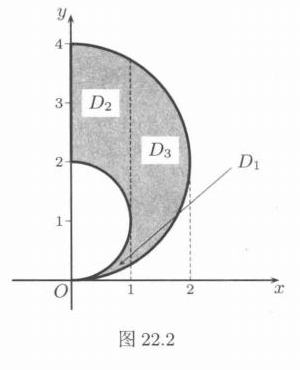
\includegraphics[width=.34\linewidth]{figures/lower/ch22/fig-22-2.png}\qquad
  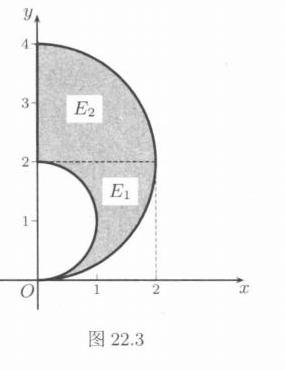
\includegraphics[width=.34\linewidth]{figures/lower/ch22/fig-22-3.png}
\end{center}
\end{xsolution}

当 $f(x,y)$ 中含有 $x^2+y^2$ 项或 $D$ 的边界表达式中有 $x^2+y^2$ 项，则可利用
\begin{equation}
  \iint_D f(x,y)\,\dd x\,\dd y
  =\iint_D f(r\cos\theta,r\sin\theta)r\,\dd r\,\dd\theta
  \tag{22.3}
  \label{eq:22.3}
\end{equation}
先化为极坐标下的二重积分，然后化为关于 $r$ 和 $\theta$ 的二次积分去求解。

\begin{xexample}[22.2.4]
将例题 22.2.3 中的区域 $D$ 分解为 $\theta$ 型区域与 $r$ 型区域。
\end{xexample}
\begin{xsolution}
在极坐标系中，$D$ 的边界
\[
  x^2+y^2=2y,\quad x^2+y^2=4y,\quad x=0
\]
分别为
\[
  r=2\sin\theta,\quad r=4\sin\theta,\quad \theta=\frac\pi2.
\]
于是表示为 $\theta$ 型区域是
\[
  0\le\theta\le\frac\pi2,\qquad 2\sin\theta\le r\le4\sin\theta;
\]
表示为 $r$ 型区域（见图 22.4）：
\[
  D_1=\begin{cases}
    0\le r\le2,\\
    \arcsin\frac r4\le\theta\le\arcsin\frac r2,
  \end{cases}
  \qquad
  D_2=\begin{cases}
    2\le r\le4,\\
    \arcsin\frac r4\le\theta\le\frac\pi2.
  \end{cases}
\]
\begin{center}
  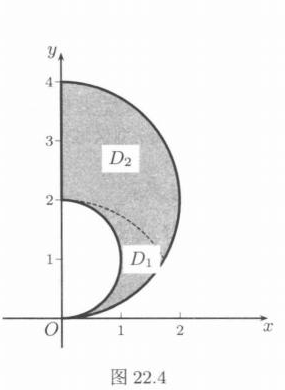
\includegraphics[width=.34\linewidth]{figures/lower/ch22/fig-22-4.png}
\end{center}
\end{xsolution}

\begin{xexample}[22.2.5]
求
\[
  \lim_{R\to+\infty}\iint_{\substack{\abs{x}\le R\\\abs{y}\le R}}(x^2+y^2)\ee^{-(x^2+y^2)}\,\dd x\,\dd y.
\]
\end{xexample}
\begin{xsolution}
记
\[
  I_R=\iint_{\substack{\abs{x}\le R\\\abs{y}\le R}}(x^2+y^2)\ee^{-(x^2+y^2)}\,\dd x\,\dd y,
\]
\[
  C_R=\iint_{x^2+y^2\le R^2}(x^2+y^2)\ee^{-(x^2+y^2)}\,\dd x\,\dd y,
\]
则 $C_R\le I_R\le C_{2R}$，且
\begin{align*}
  C_R&=\int_0^{2\pi}\dd\theta\int_0^R r^3\ee^{-r^2}\,\dd r
  =\pi\int_0^{R^2}t\ee^{-t}\,\dd t\\
  &=\pi(1-\ee^{-R^2}-R^2\ee^{-R^2})\to\pi\qquad(R\to+\infty).
\end{align*}
同理可证 $C_{2R}\to\pi$ $(R\to+\infty)$。于是
\[
  \lim_{R\to+\infty}I_R=\pi.
\]
\end{xsolution}

\begin{xexample}[22.2.6]
作极坐标变换，将二重积分
\[
  \iint_D f(\sqrt{x^2+y^2})\,\dd x\,\dd y
\]
化为定积分，其中 $D=\{(x,y)\mid0\le y\le x\le1\}$。
\end{xexample}
\begin{xsolution}
令 $x=r\cos\varphi,y=r\sin\varphi$，则
\begin{align*}
  \iint_D f(\sqrt{x^2+y^2})\,\dd x\,\dd y
  &=\iint_D f(r)r\,\dd r\,\dd\varphi\\
  &=\int_0^1\dd r\int_0^{\pi/4}f(r)r\,\dd\varphi
  +\int_1^{\sqrt2}\dd r\int_{\arccos(1/r)}^{\pi/4}f(r)r\,\dd\varphi\\
  &=\frac\pi4\int_0^1f(r)r\,\dd r
  +\int_1^{\sqrt2}\left(\frac\pi4-\arccos\frac1r\right)f(r)r\,\dd r\\
  &=\frac\pi4\int_0^{\sqrt2}f(r)r\,\dd r
  -\int_1^{\sqrt2}\arccos\frac1r f(r)r\,\dd r.
\end{align*}
\end{xsolution}

\subsection{二重积分的变量替换}

极坐标变换（见 (22.3) 式）是一种特殊的变量替换，下面是一般的变量替换定理。设
\[
  x=x(u,v),\qquad y=y(u,v),\qquad (u,v)\in D',
\]
这一代换满足：
\begin{enumerate}[label=(\arabic*)]
  \item 建立了 $D$ 与 $D'$ 之间的一一对应；
  \item $x,y$ 在 $D'$ 上具有关于各个变元的连续偏导数，并且其逆变换 $u=u(x,y),v=v(x,y)$ 在 $D$ 上也具有关于各个变元的连续偏导数；
  \item 代换的 Jacobi 行列式 $J=\dfrac{\partial(x,y)}{\partial(u,v)}$ 在 $D'$ 内无零点（称这代换为正则），则
\end{enumerate}
\begin{equation}
  \iint_D f(x,y)\,\dd x\,\dd y
  =\iint_{D'} f(x(u,v),y(u,v))\abs*{\frac{\partial(x,y)}{\partial(u,v)}}\,\dd u\,\dd v.
  \tag{22.4}
  \label{eq:22.4}
\end{equation}
回忆一下一元定积分的变量替换公式，容易看出公式 (22.4) 是定积分的变量替换公式的推广。定理的证明要比一元情况复杂得多，请参考相应的教科书。

\begin{xexample}[22.2.7]
求由曲线
\[
  \left(\frac{x^2}{a^2}+\frac{y^2}{b^2}\right)^2=\frac{x^2}{a^2}-\frac{y^2}{b^2}
\]
所围的面积。
\end{xexample}
\begin{xsolution}
应用广义极坐标变换
\[
  x=a\rho\cos\theta,\qquad y=b\rho\sin\theta,
\]
则 $J=\abs*{\frac{\partial(x,y)}{\partial(u,v)}}=ab\rho$，所围成积分区域的曲线变为 $\rho^2=\cos2\theta$（双纽线），于是所求的面积
\[
  S=\iint_D\dd x\,\dd y
  =4\int_0^{\pi/4}\dd\theta\int_0^{\sqrt{\cos2\theta}}ab\rho\,\dd\rho=ab.
\]
\end{xsolution}

\begin{xexample}[22.2.8]
求
\[
  \iint_D\left(\sqrt{\frac{x-c}{a}}+\sqrt{\frac{y-c}{b}}\right)\dd x\,\dd y,
\]
其中 $D$ 由曲线 $\sqrt{\frac{x-c}{a}}+\sqrt{\frac{y-c}{b}}=1$ 和 $x=c,y=c$ 所围成，并且 $a,b,c>0$。
\end{xexample}
\begin{xsolution}
见图 22.5，被积函数与积分区域的部分边界具有相同的形式，因此要设法把被积函数表达式化成简单的形式。
\begin{center}
  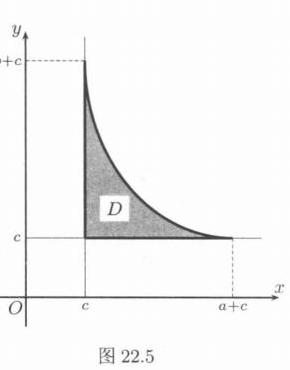
\includegraphics[width=.34\linewidth]{figures/lower/ch22/fig-22-5.png}
\end{center}
令
\[
  x=c+a\rho\cos^4\theta,\qquad y=c+b\rho\sin^4\theta,
\]
则
\[
  J=\abs*{\frac{\partial(x,y)}{\partial(\rho,\theta)}}=4ab\rho\cos^3\theta\sin^3\theta,
\]
而积分区域变为 $\{0\le\theta\le\frac\pi2,0\le\rho\le1\}$，于是
\[
  \iint_D\left(\sqrt{\frac{x-c}{a}}+\sqrt{\frac{y-c}{b}}\right)\dd x\,\dd y
  =\int_0^{\pi/2}\dd\theta\int_0^1 4ab\rho\cos^3\theta\sin^3\theta\sqrt\rho\,\dd\rho
  =\frac{2ab}{15}.
\]
\end{xsolution}

\begin{xremark}
一般而言，广义极坐标变换
\[
  x=\frac1a\left(c+r^{1/p}\cos^{2/p}\theta\right),\qquad
  y=\frac1b\left(d+r^{1/p}\sin^{2/p}\theta\right),
\]
能把 $(ax-c)^p+(by-d)^p$ 变为 $r$，但其中的 $r,\theta$ 一般不再具有通常的极径、极角的意义。
\end{xremark}

\begin{xexample}[22.2.9]
求 $I=\iint_\Omega(x+y)\,\dd x\,\dd y$，其中 $\Omega$ 是由 $y^2=2x,x+y=4,x+y=12$ 围成。
\end{xexample}
\begin{xsolution}
积分区域如图 22.6，作变换
\[
  u=x+y,\qquad v=y,
\]
则变换后的积分区域为
\[
  4\le u\le12,\qquad -1-\sqrt{2u+1}\le v\le-1+\sqrt{2u+1},
\]
且 $J=\abs*{\frac{\partial(x,y)}{\partial(u,v)}}=1$。于是
\begin{align*}
  I&=\int_4^{12}u\,\dd u\int_{-1-\sqrt{2u+1}}^{-1+\sqrt{2u+1}}\dd v\\
   &=\int_4^{12}2u\sqrt{2u+1}\,\dd u\qquad(\sqrt{2u+1}=t)\\
   &=\int_3^5(t^2-1)t^2\,\dd t=\frac{8156}{15}.
\end{align*}
\begin{center}
  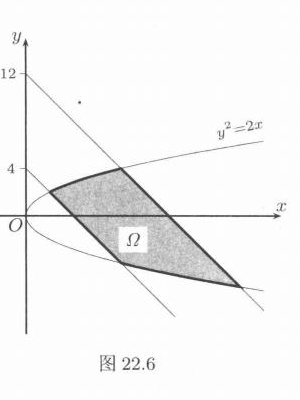
\includegraphics[width=.42\linewidth]{figures/lower/ch22/fig-22-6.png}
\end{center}
\end{xsolution}

函数的奇偶性和积分区域的对称性常可用来简化积分的计算，如
\begin{enumerate}
  \item 积分区域 $D$ 关于 $x$ 轴对称，且有：(1) $f(x,y)=-f(x,-y)$，则 $\iint_Df(x,y)\,\dd x\,\dd y=0$；(2) $f(x,y)=f(x,-y)$，则
  \[
    \iint_Df(x,y)\,\dd x\,\dd y
    =2\iint_{D\cap\{y\ge0\}}f(x,y)\,\dd x\,\dd y.
  \]
  \item 积分区域 $D$ 关于 $y$ 轴对称，且有：(1) $f(x,y)=-f(-x,y)$，则 $\iint_Df(x,y)\,\dd x\,\dd y=0$；(2) $f(x,y)=f(-x,y)$，则
  \[
    \iint_Df(x,y)\,\dd x\,\dd y
    =2\iint_{D\cap\{x\ge0\}}f(x,y)\,\dd x\,\dd y.
  \]
  \item 若 $D$ 关于原点对称，且有：(1) $f(x,y)=-f(-x,-y)$，则 $\iint_Df(x,y)\,\dd x\,\dd y=0$；(2) $f(x,y)=f(-x,-y)$，则
  \[
    \iint_Df(x,y)\,\dd x\,\dd y=2\iint_{D_1}f(x,y)\,\dd x\,\dd y,
  \]
  其中 $D_1$ 是区域 $D$ 的一半。
\end{enumerate}

\subsection{练习题}

\begin{xexercise}[1]
试把累次积分
  \[
    I=\int_0^{R/\sqrt{1+R^2}}\dd x\int_0^{Rx}f(x,y)\,\dd y
    +\int_{R/\sqrt{1+R^2}}^R\dd x\int_0^{\sqrt{R^2-x^2}}f(x,y)\,\dd y
  \]
  改写为先对 $x$ 后对 $y$ 的累次积分形式。
\end{xexercise}
\begin{xsolution}
原积分区域位于第一象限，由直线 $y=Rx$、圆 $x^2+y^2=R^2$ 和 $x$ 轴围成。直线与圆的交点为
\[
  \left(\frac{R}{\sqrt{1+R^2}},\frac{R^2}{\sqrt{1+R^2}}\right).
\]
固定 $y$ 后，有
\[
  \frac yR\le x\le\sqrt{R^2-y^2},
  \qquad0\le y\le\frac{R^2}{\sqrt{1+R^2}}.
\]
所以
\[
  \boxed{
  I=\int_0^{R^2/\sqrt{1+R^2}}\dd y
  \int_{y/R}^{\sqrt{R^2-y^2}}f(x,y)\,\dd x }.
\]
\end{xsolution}


\begin{xexercise}[2]
设 $f(x)$ 在 $[0,1]$ 上连续，证明：
  \[
    \int_0^1\dd x\int_x^1 f(t)\,\dd t=\int_0^1 t f(t)\,\dd t.
  \]
\end{xexercise}
\begin{xsolution}
积分区域为 $0\le x\le t\le1$。交换积分次序得
\begin{align*}
  \int_0^1\dd x\int_x^1f(t)\,\dd t
  &=\int_0^1\dd t\int_0^t f(t)\,\dd x\\
  &=\int_0^1t f(t)\,\dd t.
\end{align*}
\end{xsolution}


\begin{xexercise}[3]
$D$ 由 $y=\pi-x,x=\pi,y=\pi$ 围成，求 $\displaystyle\iint_D\frac{\sin x}{x}\,\dd x\,\dd y$。
\end{xexercise}
\begin{xsolution}
三条边围成的三角形可写成
\[
  0\le x\le\pi,\qquad \pi-x\le y\le\pi.
\]
故
\begin{align*}
  \iint_D\frac{\sin x}{x}\,\dd x\,\dd y
  &=\int_0^\pi\frac{\sin x}{x}\bigl[\pi-(\pi-x)\bigr]\,\dd x\\
  &=\int_0^\pi\sin x\,\dd x=\boxed{2}.
\end{align*}
$x=0$ 处按连续延拓理解即可。
\end{xsolution}


\begin{xexercise}[4]
$D$ 由 $y=0,y=x^2,x+y=2$ 围成的第一象限的部分，求 $\displaystyle\iint_D(x^2+y^2)\,\dd x\,\dd y$。
\end{xexercise}
\begin{xsolution}
曲线 $y=x^2$ 与直线 $x+y=2$ 在第一象限交于 $(1,1)$。因此
\[
  D=\{0\le x\le1,0\le y\le x^2\}
  \cup\{1\le x\le2,0\le y\le2-x\}.
\]
于是
\begin{align*}
 I&=\int_0^1\int_0^{x^2}(x^2+y^2)\,\dd y\,\dd x
 +\int_1^2\int_0^{2-x}(x^2+y^2)\,\dd y\,\dd x\\
 &=\int_0^1\left(x^4+\frac{x^6}{3}\right)\dd x
 +\int_1^2\left[x^2(2-x)+\frac{(2-x)^3}{3}\right]\dd x\\
 &=\frac{26}{105}+1=\boxed{\frac{131}{105}}.
\end{align*}
\end{xsolution}


\begin{xexercise}[5]
求由 $(x^2+y^2)^2=a^2(x^2-y^2),z=x^2-y^2,z=0$ 围成之立体的体积。
\end{xexercise}
\begin{xsolution}
在极坐标下，边界曲线变为
\[
  r^4=a^2r^2\cos2\theta,
  \qquad r^2=a^2\cos2\theta.
\]
它有关于 $x$ 轴正、负方向的两个全等叶瓣；在叶瓣内 $x^2-y^2=r^2\cos2\theta\ge0$，故立体高度为 $r^2\cos2\theta$。于是
\begin{align*}
 V&=2\int_{-\pi/4}^{\pi/4}\int_0^{a\sqrt{\cos2\theta}}
 r^2\cos2\theta\,r\,\dd r\,\dd\theta\\
 &=\frac{a^4}{2}\int_{-\pi/4}^{\pi/4}\cos^3 2\theta\,\dd\theta
 =\frac{a^4}{4}\int_{-\pi/2}^{\pi/2}\cos^3u\,\dd u\\
 &=\boxed{\frac{a^4}{3}}.
\end{align*}
\end{xsolution}


\begin{xexercise}[6]
设 $D$ 是由 $x^2=ay,x^2=by,y^2=px,y^2=qx$ 所围成的区域，其中 $0<a<b,0<p<q$，求
  \[
    \iint_D\frac{x^2\sin xy}{y}\,\dd x\,\dd y.
  \]
\end{xexercise}
\begin{xsolution}
区域位于第一象限。作变换
\[
  u=\frac{x^2}{y},\qquad v=\frac{y^2}{x}.
\]
四族边界分别为 $u=a,u=b,v=p,v=q$，而
\[
  uv=xy,
  \qquad
  \frac{\partial(u,v)}{\partial(x,y)}=3.
\]
故 $\dd x\,\dd y=\frac13\dd u\,\dd v$，且
\begin{align*}
 I&=\frac13\int_a^b\int_p^q u\sin(uv)\,\dd v\,\dd u\\
 &=\frac13\int_a^b\bigl[\cos(pu)-\cos(qu)\bigr]\,\dd u\\
 &=\boxed{\frac13\left[
 \frac{\sin(bp)-\sin(ap)}p-
 \frac{\sin(bq)-\sin(aq)}q\right]}.
\end{align*}
\end{xsolution}


\begin{xexercise}[7]
证明：
  \[
    \int_a^b\dd y\int_a^y(y-x)^n f(x)\,\dd x
    =\frac1{n+1}\int_a^b(b-x)^{n+1}f(x)\,\dd x.
  \]
\end{xexercise}
\begin{xsolution}
原积分区域为 $a\le x\le y\le b$。交换积分次序：$a\le x\le b$，$x\le y\le b$。于是（$n$ 为非负整数）
\begin{align*}
 \int_a^b\dd y\int_a^y(y-x)^nf(x)\,\dd x
 &=\int_a^b f(x)\,\dd x\int_x^b(y-x)^n\,\dd y\\
 &=\frac1{n+1}\int_a^b(b-x)^{n+1}f(x)\,\dd x.
\end{align*}
\end{xsolution}


\begin{xexercise}[8]
设 $D$ 是第一象限内由 $y$ 轴及两个圆 $x^2+y^2=a^2,x^2-2ax+y^2=0$ 所围成的区域，求 $\displaystyle\iint_D\sqrt{x^2+y^2}\,\dd x\,\dd y$。
\end{xexercise}
\begin{xsolution}
在第一象限，两圆分别为
\[
  r=a,
  \qquad r=2a\cos\theta.
\]
它们在 $\theta=\pi/3$ 相交。由 $y$ 轴封闭的区域为
\[
  \frac\pi3\le\theta\le\frac\pi2,
  \qquad2a\cos\theta\le r\le a.
\]
被积函数为 $r$，故
\begin{align*}
 I&=\int_{\pi/3}^{\pi/2}\int_{2a\cos\theta}^{a}r^2\,\dd r\,\dd\theta\\
 &=\frac{a^3}{3}\left[\frac\pi6-8\int_{\pi/3}^{\pi/2}\cos^3\theta\,\dd\theta\right]\\
 &=\boxed{\frac{a^3}{18}\left(\pi+18\sqrt3-32\right)}.
\end{align*}
\end{xsolution}


\begin{xexercise}[9]
求由四条直线 $x+y=p,x+y=q,y=ax,y=bx$（$0<p<q,0<a<b$）所围成的图形的面积。
\end{xexercise}
\begin{xsolution}
令
\[
  u=x+y,\qquad v=\frac yx.
\]
则 $p\le u\le q$，$a\le v\le b$，且
\[
  x=\frac{u}{1+v},\qquad y=\frac{uv}{1+v},
  \qquad
  \abs*{\frac{\partial(x,y)}{\partial(u,v)}}=\frac{u}{(1+v)^2}.
\]
所以所求面积
\begin{align*}
 S&=\int_p^q\int_a^b\frac{u}{(1+v)^2}\,\dd v\,\dd u\\
 &=\frac{q^2-p^2}{2}\left(\frac1{1+a}-\frac1{1+b}\right)\\
 &=\boxed{\frac{(q^2-p^2)(b-a)}{2(1+a)(1+b)}}.
\end{align*}
\end{xsolution}


\begin{xexercise}[10]
求由曲线 $\sqrt[4]{x/a}+\sqrt[4]{y/b}=1$ 与直线 $x=0,y=0$ 所围成图形的面积。
\end{xexercise}
\begin{xsolution}
令
\[
  u=\sqrt[4]{x/a},\qquad v=\sqrt[4]{y/b}.
\]
则 $x=au^4,y=bv^4$，区域变为
\[
  u\ge0,\quad v\ge0,\quad u+v\le1,
\]
且
\[
  \abs*{\frac{\partial(x,y)}{\partial(u,v)}}=16ab\,u^3v^3.
\]
故
\begin{align*}
 S&=16ab\int_0^1u^3\,\dd u\int_0^{1-u}v^3\,\dd v\\
 &=4ab\int_0^1u^3(1-u)^4\,\dd u
 =4ab\cdot\frac1{280}=\boxed{\frac{ab}{70}}.
\end{align*}
\end{xsolution}


\begin{xexercise}[11]
求 $\displaystyle\iint_D f(\sqrt{x^2+y^2})\,\dd x\,\dd y$，其中 $D=\{(x,y)\mid\abs{y}<\abs{x}\le1\}$。
\end{xexercise}
\begin{xsolution}
区域由关于正、负 $x$ 轴的两个全等扇形状部分组成。极坐标下，角度范围为
\[
 -\frac\pi4\le\theta\le\frac\pi4,
 \qquad
 \frac{3\pi}{4}\le\theta\le\frac{5\pi}{4},
\]
且 $r\abs{\cos\theta}\le1$。对 $0\le r\le1$，可取的角度总长为 $\pi$；对 $1\le r\le\sqrt2$，可取的角度总长为
\[
  \pi-4\arccos\frac1r.
\]
因此
\[
 \boxed{
 \iint_Df(\sqrt{x^2+y^2})\,\dd x\,\dd y
 =\pi\int_0^{\sqrt2}f(r)r\,\dd r
 -4\int_1^{\sqrt2}\arccos\frac1r\,f(r)r\,\dd r }.
\]
\end{xsolution}


\begin{xexercise}[12]
求 $\displaystyle\iint_D x\,\dd x\,\dd y$，其中 $D$ 由 $xy=1,x^2+y^2=4$ 围成。
\end{xexercise}
\begin{xsolution}
由 $xy=1$ 与 $x^2+y^2=4$ 围成的整个区域关于原点对称，而被积函数 $x$ 满足
\[
  x(-x,-y)=-x(x,y).
\]
故两对称部分的积分互相抵消，
\[
  \boxed{\iint_Dx\,\dd x\,\dd y=0}.
\]
\end{xsolution}


\begin{xexercise}[13]
给定积分
  \[
    I=\iint_D\left[\left(\frac{\partial f}{\partial x}\right)^2+\left(\frac{\partial f}{\partial y}\right)^2\right]\dd x\,\dd y,
  \]
  作正则变换 $x=x(u,v),y=y(u,v)$，区域 $D$ 变为 $\Omega$，如果变换满足
  \[
    \frac{\partial x}{\partial u}=\frac{\partial y}{\partial v},\qquad
    \frac{\partial x}{\partial v}=-\frac{\partial y}{\partial u},
  \]
  证明：
  \[
    I=\iint_\Omega\left[\left(\frac{\partial f}{\partial u}\right)^2+\left(\frac{\partial f}{\partial v}\right)^2\right]\dd u\,\dd v.
  \]
\end{xexercise}
\begin{xsolution}
记
\[
 a=x_u=y_v,
 \qquad b=x_v=-y_u.
\]
正则性给出
\[
 J=\frac{\partial(x,y)}{\partial(u,v)}=x_uy_v-x_vy_u=a^2+b^2>0.
\]
由链式法则
\[
 f_u=f_xa-f_yb,
 \qquad
 f_v=f_xb+f_ya,
\]
故
\[
 f_u^2+f_v^2=(a^2+b^2)(f_x^2+f_y^2)=J(f_x^2+f_y^2).
\]
又 $\dd x\,\dd y=J\,\dd u\,\dd v$，所以
\[
 \iint_D(f_x^2+f_y^2)\,\dd x\,\dd y
 =\iint_\Omega(f_u^2+f_v^2)\,\dd u\,\dd v.
\]
\end{xsolution}


\begin{xexercise}[14]
求积分
  \[
    \int_0^{\sqrt2}\dd y\int_y^{\sqrt{4-y^2}}\frac{1}{\sqrt{1+x^2+y^2}}\,\dd x.
  \]
\end{xexercise}
\begin{xsolution}
积分区域满足 $x\ge y\ge0$ 且 $x^2+y^2\le4$，即极坐标下
\[
 0\le\theta\le\frac\pi4,
 \qquad0\le r\le2.
\]
于是
\begin{align*}
 I&=\int_0^{\pi/4}\int_0^2\frac{r}{\sqrt{1+r^2}}\,\dd r\,\dd\theta\\
 &=\frac\pi4\left[\sqrt{1+r^2}\right]_0^2
 =\boxed{\frac\pi4(\sqrt5-1)}.
\end{align*}
\end{xsolution}


\begin{xexercise}[15]
证明：
  \[
    \iint_{\abs{x}+\abs{y}\le1}(\sqrt{\abs{xy}}+\abs{xy})\,\dd x\,\dd y\le\frac32.
  \]
\end{xexercise}
\begin{xsolution}
由四象限对称性，
\begin{align*}
 I&=4\int_0^1\int_0^{1-x}(\sqrt{xy}+xy)\,\dd y\,\dd x\\
 &=\frac83\int_0^1x^{1/2}(1-x)^{3/2}\,\dd x
 +2\int_0^1x(1-x)^2\,\dd x\\
 &=\frac83B\left(\frac32,\frac52\right)+\frac16
 =\frac\pi6+\frac16.
\end{align*}
因此
\[
 I=\frac{\pi+1}{6}<\frac32,
\]
所要求的不等式成立。
\end{xsolution}


\begin{xexercise}[16]
计算二重积分
  \[
    I=\iint_D\abs{x-y^2}\,\dd x\,\dd y,
  \]
  其中 $D=\{(x,y)\mid0\le x\le1,-1\le y\le1\}$。
\end{xexercise}
\begin{xsolution}
固定 $y$，令 $a=y^2\in[0,1]$，则
\[
 \int_0^1\abs{x-y^2}\,\dd x
 =\int_0^a(a-x)\,\dd x+\int_a^1(x-a)\,\dd x
 =a^2-a+\frac12.
\]
故
\begin{align*}
 I&=\int_{-1}^1\left(y^4-y^2+\frac12\right)\dd y\\
 &=2\left(\frac15-\frac13+\frac12\right)
 =\boxed{\frac{11}{15}}.
\end{align*}
\end{xsolution}


\begin{xexercise}[17]
求 $\displaystyle\iint_D\abs*{\ln\frac{x}{y^2}}\,\dd x\,\dd y$，其中 $D$ 是由 $y=x,y=1,x=2$ 围成的三角形。
\end{xexercise}
\begin{xsolution}
三角形可写成
\[
 1\le x\le2,
 \qquad1\le y\le x.
\]
在其中 $\ln(x/y^2)$ 的变号曲线为 $y=\sqrt x$。于是
\begin{align*}
 I&=\int_1^2\left[
 \int_1^{\sqrt x}\ln\frac{x}{y^2}\,\dd y
 -\int_{\sqrt x}^{x}\ln\frac{x}{y^2}\,\dd y
 \right]\dd x\\
 &=\boxed{\frac{64\sqrt2-89}{12}}.
\end{align*}
例如使用原函数
\[
 \int\ln\frac{x}{y^2}\,\dd y
 =y\ln x-2y\ln y+2y
\]
代入三个端点即可得到上述结果。
\end{xsolution}


\section{\texorpdfstring{三重积分，$n$ 重积分}{三重积分，n 重积分}}

三重积分的定义与二重积分类似，这里不再重复。

\subsection{三重积分在直角坐标系中的计算}

1. 先一后二：即先做一次关于某个变量的单积分，然后做关于另外两个变量的二重积分。

设 $\Omega$ 是 $\RR^3$ 中的有界区域，假设平行于 $z$ 轴且穿过闭区域 $\Omega$ 内部的直线与 $\Omega$ 的边界相交不多于两点。把 $\Omega$ 投影到 $xOy$ 平面上，得一平面闭区域 $D$，即（见图 22.7）：
\[
  \Omega=\{(x,y,z)\mid(x,y)\in D,\ z_1(x,y)\le z\le z_2(x,y)\},
\]
其中 $z_1(x,y),z_2(x,y)$ 在 $D$ 上连续。如果 $f(x,y,z)$ 在 $\Omega$ 上有界可积，且对任意 $(x,y)\in D$，$f(x,y,z)$ 作为 $z$ 的函数在 $[z_1(x,y),z_2(x,y)]$ 上可积，则
\[
  \iiint_\Omega f(x,y,z)\,\dd x\,\dd y\,\dd z
  =\iint_D\dd x\,\dd y\int_{z_1(x,y)}^{z_2(x,y)}f(x,y,z)\,\dd z.
\]
此种积分方法称为“先一后二”。
\begin{center}
  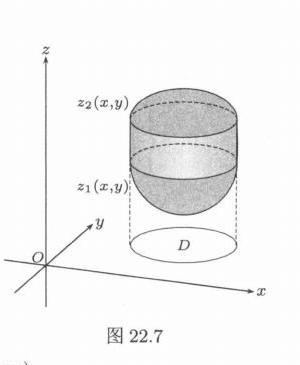
\includegraphics[width=.34\linewidth]{figures/lower/ch22/fig-22-7.png}
\end{center}

2. 先二后一：即先作关于某两个变量的二重积分，然后做关于另一个变量的单积分。这种积分方法对区域没有任何特殊要求。设
\[
  \Omega=\{(x,y,z)\mid a\le z\le b,(x,y)\in D(z)\},
\]
其中 $D(z)$ 是 $xOy$ 平面上随 $z$ 连续变化的有界闭区域。如果 $f(x,y,z)$ 在 $\Omega$ 上有界可积，对任意 $z\in[a,b]$，$f(x,y,z)$ 作为 $x,y$ 的函数在 $D(z)$ 上可积，则
\[
  \iiint_\Omega f(x,y,z)\,\dd x\,\dd y\,\dd z
  =\int_a^b\dd z\iint_{D(z)}f(x,y,z)\,\dd x\,\dd y.
\]

对这个公式可这样来理解：把 $\Omega$ 看作是一个物质立体，$f(x,y,z)$ 为物质在 $\Omega$ 上的分布密度，那么上式左端的三重积分就是物质立体的质量。而上式右端则表明先把立体切成薄片，再把所有薄片的质量积累起来。

当然，我们不一定非固定 $z$ 而先计算关于 $x,y$ 的二重积分不可，也可根据被积函数的具体情况和积分域的构成，把 $y$（或 $x$）固定而先计算关于 $z,x$（或 $y,z$）的二重积分。

\begin{xexample}[22.3.1]
求积分
\[
  I=\iiint_\Omega z^2\,\dd x\,\dd y\,\dd z,
\]
其中 $\Omega$ 为两个球 $x^2+y^2+z^2\le R^2$，$x^2+y^2+z^2\le2Rz$ 的公共部分。
\end{xexample}
\begin{xsolution}
先画出积分区域，如图 22.8。
\begin{center}
  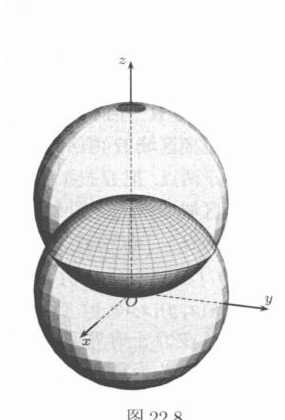
\includegraphics[width=.38\linewidth]{figures/lower/ch22/fig-22-8.png}
\end{center}
综合被积函数和积分区域，可把积分视成在 $z\in[0,R]$ 上一系列带权 $z^2$ 的小薄片的求和。根据积分区域 $\Omega$ 的构成情况，可将 $\Omega$ 分成两个子区域 $\Omega_1$ 与 $\Omega_2$：
\[
  \Omega_1:\begin{cases}
    x^2+y^2+z^2\le2Rz,\\
    0\le z\le\dfrac R2,
  \end{cases}
  \qquad
  \Omega_2:\begin{cases}
    x^2+y^2+z^2\le R^2,\\
    \dfrac R2\le z\le R.
  \end{cases}
\]
当 $z\in[0,R/2]$ 时，由 $x^2+y^2+z^2\le2Rz$ 可得到薄片面积为 $\pi(2Rz-z^2)$；当 $z\in[R/2,R]$ 时，由 $x^2+y^2+z^2\le R^2$ 可得到薄片面积为 $\pi(R^2-z^2)$。所以
\begin{align*}
  I&=\int_0^{R/2}\pi z^2(2Rz-z^2)\,\dd z
  +\int_{R/2}^R\pi z^2(R^2-z^2)\,\dd z\\
  &=\left(\frac12\pi Rz^4-\frac15\pi z^5\right)_0^{R/2}
  +\left(\frac13\pi R^2z^3-\frac15\pi z^5\right)_{R/2}^R
  =\frac{59}{480}\pi R^5.
\end{align*}
\end{xsolution}

\subsection{三重积分的变量替换}

类似于二重积分的变量替换，有如下三重积分变量替换定理。设
\[
  x=x(u,v,w),\qquad y=y(u,v,w),\qquad z=z(u,v,w),\qquad (u,v,w)\in\Omega'.
\]
这一代换满足：
\begin{enumerate}[label=(\arabic*)]
  \item 建立了 $\Omega$ 与 $\Omega'$ 之间的一一对应；
  \item $x,y,z$ 在 $\Omega'$ 上关于各个变元有连续偏导数，并且逆变换 $u=u(x,y,z),v=v(x,y,z),w=w(x,y,z)$ 在 $\Omega$ 上也关于各个变元有连续偏导数；
  \item 代换的 Jacobi 行列式 $J=\dfrac{\partial(x,y,z)}{\partial(u,v,w)}$ 在 $\Omega'$ 内没有零点，则
\end{enumerate}
\[
  \iiint_\Omega f(x,y,z)\,\dd x\,\dd y\,\dd z
  =\iiint_{\Omega'}f(x(u,v,w),y(u,v,w),z(u,v,w))
  \abs*{\frac{\partial(x,y,z)}{\partial(u,v,w)}}\,\dd u\,\dd v\,\dd w.
\]

常用的三重积分变换有下列两个。

\textbf{(1) 柱坐标变换}
\[
  x=\rho\cos\theta,\qquad y=\rho\sin\theta,\qquad z=z,
\]
\[
  0\le\rho<+\infty,\quad0\le\theta<2\pi,\quad-\infty<z<+\infty.
\]
空间直角坐标系下的三重积分与柱坐标系下的三重积分的关系是
\[
  \iiint_\Omega f(x,y,z)\,\dd x\,\dd y\,\dd z
  =\iiint_{\Omega'}f(\rho\cos\theta,\rho\sin\theta,z)\rho\,\dd\rho\,\dd\theta\,\dd z.
\]
如果积分区域为柱形或被积函数中含有 $x^2+y^2$ 项，则往往将积分在柱坐标系中计算。在计算时，常常是把三重积分化为对 $z$ 的单积分与关于 $\rho,\theta$ 的二重积分来计算，至于是“先一后二”，还是“先二后一”，那要看具体情况。

我们可以看出，柱坐标变换就是 $z$ 不变，而将 $x,y$ 用极坐标变换。在二重积分中我们曾提到广义极坐标变换，因此对应过来也有广义柱坐标变换。

\textbf{(2) 球坐标变换}
\[
  x=\rho\sin\varphi\cos\theta,\qquad
  y=\rho\sin\varphi\sin\theta,\qquad
  z=\rho\cos\varphi,
\]
\[
  0\le\rho<+\infty,\qquad0\le\theta<2\pi,\qquad0\le\varphi\le\pi.
\]
空间直角坐标系下的三重积分与球坐标系下的三重积分的关系是
\[
  \iiint_\Omega f(x,y,z)\,\dd x\,\dd y\,\dd z
  =\iiint_{\Omega'}f(\rho\sin\varphi\cos\theta,\rho\sin\varphi\sin\theta,\rho\cos\varphi)
  \rho^2\sin\varphi\,\dd\rho\,\dd\theta\,\dd\varphi.
\]
\begin{xremark}
利用球坐标计算三重积分，一般说来适用于积分区域是球心在原点或过原点而球心在坐标轴上的球体、顶点在原点以坐标轴为旋转轴的圆锥体以及被积函数中出现 $x^2+y^2+z^2$ 的三重积分。

使用球坐标时对 $\rho,\theta,\varphi$ 的几何意义要十分清楚。比如在我们上面给出的球坐标变换下，$\rho$ 是球半径（$0\le\rho<+\infty$），$\theta$ 是转动角（$0\le\theta<2\pi$），$\varphi$ 是仰角（与 $z$ 轴正向的夹角，$0\le\varphi\le\pi$）。在有的教科书上给出了几种不同的球坐标系，建议只取一种记忆，以免混淆。此外对应于二重积分的广义极坐标变换，也有广义球坐标变换。
\end{xremark}

\subsection{例题}

\begin{xexample}[22.3.2]
求
\[
  I=\iiint_\Omega(x+y)\,\dd x\,\dd y\,\dd z,
\]
其中 $\Omega$ 为由 $x=0,x=1,x^2+1=\frac{y^2}{a^2}+\frac{z^2}{b^2}$ 所围成。
\end{xexample}
\begin{xsolution}
由积分区域（见图 22.9）的构成宜采用“先二后一”的积分次序。
\begin{center}
  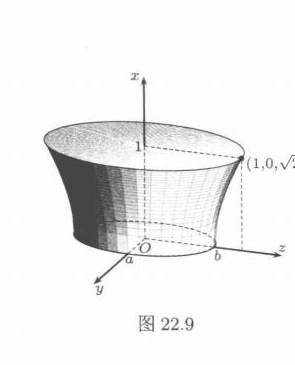
\includegraphics[width=.38\linewidth]{figures/lower/ch22/fig-22-9.png}
\end{center}
\[
  I=\int_0^1\dd x\iint_{D(x)}(x+y)\,\dd y\,\dd z,
\]
其中
\[
  D(x)=\left\{(x,y,z)\middle|\frac{y^2}{a^2}+\frac{z^2}{b^2}\le1+x^2\right\}.
\]
对于二重积分 $\iint_{D(x)}y\,\dd y\,\dd z$，由于 $D(x)$ 在 $yOz$ 平面上的投影关于原点对称，且 $f(y,z)=y=-f(-y,-z)$，由 22.2.3 小节中最后一部分关于简化积分的说明知
\[
  \iint_{D(x)}y\,\dd y\,\dd z=0,
\]
而
\[
  \iint_{D(x)}x\,\dd y\,\dd z=\pi abx(1+x^2).
\]
于是
\[
  I=\pi ab\int_0^1x(1+x^2)\,\dd x=\frac34\pi ab.
\]
\end{xsolution}

\begin{xexample}[22.3.3]
计算积分
\[
  H=\iiint_{\substack{x,y,z\ge0\\x^2+y^2+z^2\le R^2}}
  \frac{xyz\,\dd x\,\dd y\,\dd z}{\sqrt{a^2x^2+b^2y^2+c^2z^2}},
  \qquad a>b>c>0.
\]
\end{xexample}
\begin{xsolution}
在球坐标下
\[
  H=\int_0^{\pi/2}\int_0^{\pi/2}\int_0^R
  \frac{r^4\sin^3\varphi\cos\varphi\sin\theta\cos\theta\,\dd r\,\dd\varphi\,\dd\theta}
  {\sqrt{a^2\sin^2\varphi\cos^2\theta+b^2\sin^2\varphi\sin^2\theta+c^2\cos^2\varphi}}.
\]
令 $\sin^2\varphi=u,\sin^2\theta=v$，则
\begin{align*}
  H&=\frac14\int_0^1\int_0^1\int_0^R
  \frac{r^4u\,\dd r\,\dd u\,\dd v}
  {\sqrt{a^2u(1-v)+b^2uv+c^2(1-u)}}\\
  &=\frac1{20}R^5\int_0^1u\,\dd u\int_0^1
  \frac{\dd v}{\sqrt{[c^2+(a^2-c^2)u]+(b^2-a^2)uv}}\\
  &=\frac1{20}R^5\int_0^1\left\{
  \frac{2}{(b^2-a^2)u}\sqrt{[c^2+(a^2-c^2)u]+(b^2-a^2)uv}
  \right\}_{v=0}^{v=1}u\,\dd u\\
  &=\frac{R^5}{10(b^2-a^2)}\int_0^1
  \left\{\sqrt{c^2+(b^2-c^2)u}-\sqrt{c^2+(a^2-c^2)u}\right\}\dd u\\
  &=\frac{R^5}{10(b^2-a^2)}\left\{
  \frac{2}{3(b^2-c^2)}[c^2+(b^2-c^2)u]^{3/2}
  -\frac{2}{3(a^2-c^2)}[c^2+(a^2-c^2)u]^{3/2}
  \right\}_0^1\\
  &=\frac{R^5}{10(b^2-a^2)}\left[
  \frac{2}{3(b^2-c^2)}(b^3-c^3)
  -\frac{2}{3(a^2-c^2)}(a^3-c^3)\right]\\
  &=\frac{R^5}{15}\cdot\frac1{b^2-a^2}
  \left(\frac{b^2+bc+c^2}{b+c}-\frac{a^2+ac+c^2}{a+c}\right)\\
  &=\frac{R^5}{15}\cdot\frac{ab+bc+ca}{(a+b)(b+c)(c+a)}.
\end{align*}
\end{xsolution}

\begin{xexample}[22.3.4]
设
\[
  H(x)=\sum_{i,j=1}^3a_{ij}x_ix_j,
\]
$A=(a_{ij})$ 是 3 阶正定对称阵，求
\[
  I=\iiint_{H(x)\le1}\ee^{\sqrt{H(x)}}\,\dd x_1\,\dd x_2\,\dd x_3.
\]
\end{xexample}
\begin{xsolution}
存在 3 阶正交矩阵 $P$，使得
\[
  P^{\mathsf T}AP=
  \begin{pmatrix}
    \lambda_1&0&0\\
    0&\lambda_2&0\\
    0&0&\lambda_3
  \end{pmatrix},
\]
其中 $\lambda_i>0,i=1,2,3$。作正交变换 $x=Py$，这里 $x,y\in\RR^3$，则
\[
  H(x)=H(Py)=\lambda_1y_1^2+\lambda_2y_2^2+\lambda_3y_3^2,
\]
且变换的 Jacobi 行列式 $\det P=1$。从而
\[
  I=\iiint_{\lambda_1y_1^2+\lambda_2y_2^2+\lambda_3y_3^2\le1}
  \ee^{\sqrt{\lambda_1y_1^2+\lambda_2y_2^2+\lambda_3y_3^2}}\,\dd y_1\,\dd y_2\,\dd y_3.
\]
令
\[
  y_1=\frac1{\sqrt{\lambda_1}}r\sin\varphi\cos\theta,\qquad
  y_2=\frac1{\sqrt{\lambda_2}}r\sin\varphi\sin\theta,
\]
\[
  y_3=\frac1{\sqrt{\lambda_3}}r\cos\varphi,
\]
则
\begin{align*}
  I&=\frac1{\sqrt{\lambda_1\lambda_2\lambda_3}}
  \int_0^{2\pi}\dd\theta\int_0^\pi\dd\varphi\int_0^1r^2\ee^r\sin\varphi\,\dd r\\
  &=\frac{4\pi}{\sqrt{\lambda_1\lambda_2\lambda_3}}\int_0^1r^2\ee^r\,\dd r
  =\frac{4\pi}{\sqrt{\lambda_1\lambda_2\lambda_3}}(\ee-2).
\end{align*}
由于 $A$ 的行列式 $\det A=\lambda_1\lambda_2\lambda_3$，所以
\[
  I=\frac{4\pi}{\sqrt{\det A}}(\ee-2).
\]
\end{xsolution}

\begin{xremark}
正交变换是一种很有用的坐标变换。它的特点是刚体变换，仅仅旋转坐标轴，保持区域体积不变。特别是保持单位球不变。
\end{xremark}

\subsection{\texorpdfstring{$n$ 重积分}{n 重积分}}

以四重积分为例，按照三重积分的思路，可以采用“先一后三”或者“先三后一”或者“先二后二”的积分次序，而对于其中的“三”或者“二”，则采用三重积分或者二重积分化累次积分的方法。也可以用四维的变量替换。

\begin{xexample}[22.3.5]
求四维空间中的单位球
\[
  x^2+y^2+z^2+t^2\le a^2
\]
的体积 $V$。
\end{xexample}
\begin{xsolution}
用四维空间中的球坐标变换
\begin{equation}
  x=r\sin\varphi_1\sin\varphi_2\cos\theta,\qquad
  y=r\sin\varphi_1\sin\varphi_2\sin\theta,
  \tag{22.5}
  \label{eq:22.5}
\end{equation}
\begin{equation}
  z=r\sin\varphi_1\cos\varphi_2,\qquad
  t=r\cos\varphi_1,
  \tag{22.6}
  \label{eq:22.6}
\end{equation}
其中 $0\le r\le a,0\le\theta<2\pi,0\le\varphi_1,\varphi_2\le\pi$，则
\[
  \abs*{\frac{\partial(x,y,z,t)}{\partial(r,\varphi_1,\varphi_2,\theta)}}
  =r^3\sin^2\varphi_1\sin\varphi_2.
\]
于是
\begin{align*}
  V&=\iiiint_{x^2+y^2+z^2+t^2\le a^2}\dd x\,\dd y\,\dd z\,\dd t\\
  &=\int_0^{2\pi}\dd\theta\int_0^\pi\dd\varphi_1\int_0^\pi\dd\varphi_2\int_0^a
  r^3\sin^2\varphi_1\sin\varphi_2\,\dd r\\
  &=\frac{\pi a^4}{2}\int_0^\pi\sin^2\varphi_1\,\dd\varphi_1\int_0^\pi\sin\varphi_2\,\dd\varphi_2
  =\frac{\pi^2a^4}{2}.
\end{align*}
\end{xsolution}

\subsection{练习题}

\begin{xexercise}[1]
计算积分
  \[
    \int_0^1\dd x\int_0^{1-x}\dd z\int_0^{1-z-x}(1-y)\ee^{-(1-y-z)^2}\,\dd y.
  \]
\end{xexercise}
\begin{xsolution}
原积分区域为
\[
 x\ge0,\quad z\ge0,\quad y\ge0,\quad x+z+y\le1.
\]
在最内层令 $t=1-y-z$，则 $y=1-z-t$，且 $1-y=z+t$。再交换 $x,z,t$ 的次序，可写成
\[
 0\le t\le1,
 \qquad0\le x\le t,
 \qquad0\le z\le1-t.
\]
于是
\begin{align*}
 I&=\int_0^1\ee^{-t^2}\,\dd t\int_0^t\dd x\int_0^{1-t}(z+t)\,\dd z\\
 &=\frac12\int_0^1t(1-t^2)\ee^{-t^2}\,\dd t.
\end{align*}
令 $u=t^2$，得
\[
 I=\frac14\int_0^1(1-u)\ee^{-u}\,\dd u
 =\boxed{\frac1{4\ee}}.
\]
\end{xsolution}


\begin{xexercise}[2]
将累次积分
  \[
    \int_0^2\dd x\int_{-\sqrt{2x-x^2}}^0\dd y\int_0^x f(x,y,z)\,\dd z
  \]
  化为在柱坐标系下的累次积分。
\end{xexercise}
\begin{xsolution}
在 $xOy$ 平面上，
\[
 (x-1)^2+y^2\le1,
 \qquad y\le0.
\]
作柱坐标变换
\[
 x=r\cos\theta,
 \qquad y=r\sin\theta,
\]
则该半圆区域为
\[
 -\frac\pi2\le\theta\le0,
 \qquad0\le r\le2\cos\theta.
\]
又 $0\le z\le x=r\cos\theta$。所以原累次积分化为
\[
 \boxed{
 \int_{-\pi/2}^{0}\dd\theta
 \int_0^{2\cos\theta}r\,\dd r
 \int_0^{r\cos\theta}
 f(r\cos\theta,r\sin\theta,z)\,\dd z }.
\]
\end{xsolution}


\begin{xexercise}[3]
求 $\displaystyle\iiint_\Omega(x^2+y^2)\,\dd x\,\dd y\,\dd z$，其中 $\Omega$ 是由曲线 $y^2=2z,x=0$ 绕 $z$ 轴旋转而成的曲面、平面 $z=2$ 与平面 $z=8$ 所围成的区域。
\end{xexercise}
\begin{xsolution}
旋转曲面为抛物面
\[
 x^2+y^2=2z.
\]
在柱坐标下，区域为
\[
 2\le z\le8,
 \qquad0\le r\le\sqrt{2z},
 \qquad0\le\theta\le2\pi.
\]
因此
\begin{align*}
 I&=\int_2^8\int_0^{2\pi}\int_0^{\sqrt{2z}}r^2\,r\,\dd r\,\dd\theta\,\dd z\\
 &=2\pi\int_2^8 z^2\,\dd z
 =\boxed{336\pi}.
\end{align*}
\end{xsolution}


\begin{xexercise}[4]
求 $\displaystyle\iiint_\Omega xyz\,\dd x\,\dd y\,\dd z$，其中 $\Omega$ 为 $x^2+y^2+z^2\le4$ 与 $x^2+y^2+(z-2)^2\le4$ 的公共部分，且 $x\ge0,y\ge0$。
\end{xexercise}
\begin{xsolution}
用柱坐标 $x=r\cos\theta,y=r\sin\theta$。由 $x,y\ge0$ 有 $0\le\theta\le\pi/2$。记
\[
 s=\sqrt{4-r^2}.
\]
两个球的公共部分在给定 $r$ 处满足
\[
 2-s\le z\le s,
\]
故必须 $s\ge1$，即 $0\le r\le\sqrt3$。于是
\begin{align*}
 I&=\int_0^{\pi/2}\cos\theta\sin\theta\,\dd\theta
 \int_0^{\sqrt3}r^3\,\dd r\int_{2-s}^{s}z\,\dd z\\
 &=\int_0^{\sqrt3}r^3(\sqrt{4-r^2}-1)\,\dd r
 =\boxed{\frac{53}{60}}.
\end{align*}
\end{xsolution}


\begin{xexercise}[5]
求 $\displaystyle\iiint_\Omega\frac{\dd x\,\dd y\,\dd z}{r}$，其中 $\Omega$ 为一半径为 $R$ 的球，$r$ 为球外一固定点到球域内任一点的距离。
\end{xexercise}
\begin{xsolution}
设球心为 $O$，球外固定点为 $P$，$A=OP>R$。以 $OP$ 为极轴，在以 $O$ 为原点的球坐标中，球内一点到 $P$ 的距离为
\[
 r=\sqrt{A^2+s^2-2As\cos\varphi},
\]
其中 $0\le s\le R$。于是
\begin{align*}
 I&=\int_0^R s^2\,\dd s\int_0^{2\pi}\dd\theta
 \int_0^\pi\frac{\sin\varphi\,\dd\varphi}
 {\sqrt{A^2+s^2-2As\cos\varphi}}.
\end{align*}
因 $A>s$，令 $u=\cos\varphi$ 可得
\[
 \int_0^\pi\frac{\sin\varphi\,\dd\varphi}
 {\sqrt{A^2+s^2-2As\cos\varphi}}=\frac2A.
\]
故
\[
 I=\frac{4\pi}{A}\int_0^Rs^2\,\dd s
 =\boxed{\frac{4\pi R^3}{3A}}.
\]
\end{xsolution}


\begin{xexercise}[6]
计算积分
  \[
    I=\iiint_\Omega\frac{xyz}{x^2+y^2}\,\dd x\,\dd y\,\dd z,
  \]
  其中 $\Omega$ 由曲面 $(x^2+y^2+z^2)^2=a^2xy$ 与平面 $z=0$ 所围成，曲面在上方，平面在下方。
\end{xexercise}
\begin{xsolution}
采用球坐标
\[
 x=\rho\sin\varphi\cos\theta,
 \quad y=\rho\sin\varphi\sin\theta,
 \quad z=\rho\cos\varphi.
\]
由 $z\ge0$ 有 $0\le\varphi\le\pi/2$。曲面方程化为
\[
 \rho^2=\frac{a^2}{2}\sin^2\varphi\sin2\theta.
\]
故 $\sin2\theta\ge0$，即
\[
 \theta\in\left[0,\frac\pi2\right]\cup
 \left[\pi,\frac{3\pi}{2}\right],
\]
且
\[
 0\le\rho\le\frac a{\sqrt2}\sin\varphi\sqrt{\sin2\theta}.
\]
同时
\[
 \frac{xyz}{x^2+y^2}=\rho\cos\varphi\cos\theta\sin\theta.
\]
于是
\begin{align*}
 I&=\frac{a^4}{32}
 \int_0^{\pi/2}\sin^5\varphi\cos\varphi\,\dd\varphi
 \left(
 \int_0^{\pi/2}\sin^32\theta\,\dd\theta+
 \int_\pi^{3\pi/2}\sin^32\theta\,\dd\theta
 \right)\\
 &=\frac{a^4}{32}\cdot\frac16\cdot\frac43
 =\boxed{\frac{a^4}{144}}.
\end{align*}
\end{xsolution}


\begin{xexercise}[7]
求
  \[
    \iiiint_{\substack{x,y,z,u\ge0\\x^2+y^2+z^2+u^2\le1}}
    \sqrt{\frac{1-x^2-y^2-z^2-u^2}{1+x^2+y^2+z^2+u^2}}\,\dd x\,\dd y\,\dd z\,\dd u.
  \]
\end{xexercise}
\begin{xsolution}
被积函数只依赖四维半径 $r=\sqrt{x^2+y^2+z^2+u^2}$。三维单位球面 $S^3$ 的面积为 $2\pi^2$，第一卦限占 $1/16$，故角向因子为 $\pi^2/8$。于是
\[
 I=\frac{\pi^2}{8}\int_0^1r^3
 \sqrt{\frac{1-r^2}{1+r^2}}\,\dd r.
\]
令 $t=r^2$，再令 $s=\sqrt{(1-t)/(1+t)}$，则
\[
 \int_0^1t\sqrt{\frac{1-t}{1+t}}\,\dd t
 =4\int_0^1\frac{s^2(1-s^2)}{(1+s^2)^3}\,\dd s
 =1-\frac\pi4.
\]
因此
\[
 \boxed{I=\frac{\pi^2}{16}\left(1-\frac\pi4\right)
 =\frac{\pi^2(4-\pi)}{64}}.
\]
\end{xsolution}


\begin{xexercise}[8]
设
  \[
    F(t)=\iiint_{x^2+y^2+z^2\le t^2}f(x^2+y^2+z^2)\,\dd x\,\dd y\,\dd z,
  \]
  其中 $f$ 为连续函数，$f(1)=1$。证明：$F'(1)=4\pi$。
\end{xexercise}
\begin{xsolution}
球坐标下
\[
 F(t)=4\pi\int_0^t f(r^2)r^2\,\dd r.
\]
由微积分基本定理
\[
 F'(t)=4\pi t^2f(t^2).
\]
已知 $f(1)=1$，所以
\[
 \boxed{F'(1)=4\pi}.
\]
\end{xsolution}


\begin{xexercise}[9]
设 $f(x,y,z)=\sqrt{x^2+y^2+z^2}$，区域 $\Omega\subset\RR^3$ 由 $z\ge\sqrt{x^2+y^2}$ 和 $4\le x^2+y^2+z^2\le16$ 所确定，试计算函数 $f$ 关于 $\Omega$ 的积分平均值
  \[
    \frac1{\abs{\Omega}}\iiint_\Omega f(x,y,z)\,\dd x\,\dd y\,\dd z,
  \]
  其中 $\abs{\Omega}$ 是 $\Omega$ 的体积。
\end{xexercise}
\begin{xsolution}
在球坐标中，条件 $z\ge\sqrt{x^2+y^2}$ 等价于
\[
 0\le\varphi\le\frac\pi4,
\]
而球壳条件为 $2\le r\le4$。被积函数 $f=r$。由于角向因子在分子与分母中相同，积分平均值等于
\[
 \frac{\int_2^4r^3\,\dd r}{\int_2^4r^2\,\dd r}
 =\frac{(4^4-2^4)/4}{(4^3-2^3)/3}
 =\boxed{\frac{45}{14}}.
\]
\end{xsolution}


\begin{xexercise}[10]
设区域 $\Omega$ 由 $z=x^2+y^2,z=0,xy=1,xy=2,y=3x,y=4x$ 所围成，求积分
  \[
    I=\iiint_\Omega x^2y^2z\,\dd x\,\dd y\,\dd z.
  \]
\end{xexercise}
\begin{xsolution}
由 $xy=1,xy=2,y=3x,y=4x$ 围出的集合有第一、第三象限两个全等的连通分支。题目所说的“区域”按通常约定取其中一个连通分支；取第一象限分支。先对 $z$ 积分：
\[
 I=\frac12\iint_Dx^2y^2(x^2+y^2)^2\,\dd x\,\dd y.
\]
令
\[
 u=xy,
 \qquad v=\frac yx.
\]
则 $1\le u\le2,3\le v\le4$，并有
\[
 x^2+y^2=u\left(v+\frac1v\right),
 \qquad
 \dd x\,\dd y=\frac1{2v}\,\dd u\,\dd v.
\]
因此
\begin{align*}
 I&=\frac14\int_1^2u^4\,\dd u
 \int_3^4\left(v+\frac2v+\frac1{v^3}\right)\dd v\\
 &=\frac14\cdot\frac{31}{5}
 \left(\frac72+2\ln\frac43+\frac7{288}\right)\\
 &=\boxed{\frac{6293}{1152}+\frac{31}{10}\ln\frac43}.
\end{align*}
若把两个对称连通分支的并集都计入，则积分值为上述结果的 $2$ 倍。
\end{xsolution}


\begin{xexercise}[11]
利用正交变换计算三重积分 $\displaystyle\iiint_V\cos(ax+by+cz)\,\dd x\,\dd y\,\dd z$。其中 $V\colon x^2+y^2+z^2\le1$，$a,b,c$ 是不全为零的常数。
\end{xexercise}
\begin{xsolution}
令
\[
 k=\sqrt{a^2+b^2+c^2}>0.
\]
取正交变换把向量 $(a,b,c)$ 变到新坐标轴的第三轴方向。单位球在正交变换下保持不变，且
\[
 ax+by+cz=kw,
\]
其中 $w$ 为新坐标。固定 $w\in[-1,1]$ 时，截面是半径 $\sqrt{1-w^2}$ 的圆盘，故
\begin{align*}
 I&=\pi\int_{-1}^1(1-w^2)\cos(kw)\,\dd w\\
 &=\boxed{\frac{4\pi}{k^3}(\sin k-k\cos k)}.
\end{align*}
\end{xsolution}


\section{广义重积分}

\subsection{广义重积分的定义}

与上册第十二章类似，对于重积分也可作两方面的推广：无界区域上的积分和无界函数的积分。我们仅考虑 $\RR^2$ 的情况，其结论很容易推广到 $\RR^n$（$n\ge3$）中去。

先考虑无界区域上的广义二重积分。

设 $D$ 是 $\RR^2$ 中的无界区域，其边界由有限条光滑或逐段光滑曲线组成。函数 $f$ 定义在 $D$ 上，且在 $D$ 内的任何可求面积的有界子区域上可积。设 $D_r$ 是 $D$ 内的任一可求面积的有界子区域，包含 $D\cap B_r$，其中 $B_r$ 是 $\RR^2$ 中以 $r$ 为半径的闭圆盘。若极限
\[
  I=\lim_{r\to+\infty}\iint_{D_r}f(x,y)\,\dd x\,\dd y
\]
存在且有限，并与 $D_r$ 的取法无关，则称 $f$ 在 $D$ 上的（广义）积分收敛，或者称 $f$ 在 $D$ 上广义可积。否则称 $f$ 在 $D$ 上的（广义）积分发散。极限值 $I$ 称为 $f$ 在 $D$ 上的广义积分的值，记为 $\iint_Df(x,y)\,\dd x\,\dd y$。

如果函数 $f$ 非负，且在 $D$ 内的任何可求面积的有界子区域上可积，$D_n$ 是包含 $D\cap B_n$，$n=1,2,\ldots$ 的一列可求面积的有界子区域，则 $f$ 在 $D$ 上可积的充分必要条件是
\[
  \lim_{n\to\infty}\iint_{D_n}f(x,y)\,\dd x\,\dd y
\]
存在。这个条件也相当于
\[
  \sup_n\left\{\iint_{D_n}f(x,y)\,\dd x\,\dd y<+\infty\right\}.
\]

无界函数在有界区域上的广义二重积分可定义如下：

设 $D$ 为 $\RR^2$ 上的可求面积的有界区域，点 $p_0\in D$，函数 $f$ 定义在 $D\setminus\{p_0\}$ 上，且对任何点 $p_0$ 的可求面积的邻域 $\Delta$，$f$ 在 $D\setminus\Delta$ 上有界可积。如果
\[
  I=\lim_{d(\Delta)\to0}\iint_{D\setminus\Delta}f(x,y)\,\dd x\,\dd y
\]
存在且有限，并与 $\Delta$ 的取法无关，其中 $d(\Delta)$ 是 $\Delta$ 的直径，则称 $f$ 在 $D$ 上的（广义）积分收敛，或者称 $f$ 在 $D$ 上广义可积。否则称 $f$ 在 $D$ 上的（广义）积分发散。极限值 $I$ 称为 $f$ 在 $D$ 上的广义积分的值，记为 $\iint_Df(x,y)\,\dd x\,\dd y$。

\begin{xremark}
在上述定义中，还可将函数 $f$ 在 $D$ 内有一个奇点改为在 $D$ 内有一条奇线 $\gamma$，即曲线 $\gamma$ 上每一点都是 $f$ 的奇点。设 $D_l$ 是任意可以将 $\gamma$ 围起来的可求面积区域，设 $f$ 在 $D\setminus D_l$ 中可积。令 $D_l$ 收缩为 $\gamma$，记为 $D_l\to\gamma$，如果极限
\[
  \lim_{D_l\to\gamma}\iint_{D\setminus D_l}f(x,y)\,\dd x\,\dd y
\]
存在且有限，并与 $D_l$ 的取法无关，则称 $f$ 在 $D$ 上可积。设 $l$ 为 $D_l$ 的边界，其中 $D_l$ 收缩为 $\gamma$ 可理解为
\[
  \sup_{x\in l}\{\operatorname{dist}(x,\gamma)\}\to0.
\]
\end{xremark}

对于非负函数，也有与有限区域上广义重积分类似的可积充分必要条件。

\subsection{收敛性判别法}

由上节关于非负函数可积的充分必要条件，我们可以得到如下收敛性判别法：

\textbf{比较判别法}
设 $D$ 为无界区域，其边界由有限条光滑或逐段光滑曲线组成。函数 $f,g$ 在 $D$ 上有定义，对于 $D$ 内的任一可求面积的有界子区域 $D_r$，$f,g$ 均在 $D_r$ 上有界可积。如果 $g$ 非负，且
\[
  \abs{f(x,y)}\le g(x,y),\qquad\forall(x,y)\in D,
\]
则当 $g$ 在 $D$ 上（广义）可积时，$f$ 也在 $D$ 上（广义）可积。反之，如果
\[
  \abs{f(x,y)}\ge g(x,y),\qquad\forall(x,y)\in D,
\]
则当 $g$ 在 $D$ 上的广义积分发散时，$f$ 在 $D$ 上的广义积分也发散。

记 $r=\sqrt{x^2+y^2}$ 并取 $g(x,y)=\frac C{r^p}$，$C$ 为常数，由上述比较判别法可得如下判别法：

\textbf{Cauchy 判别法}
设 $D$ 为无界区域，其边界由有限条光滑或逐段光滑曲线组成，$f$ 在 $D$ 内的任一可求面积的有界子区域上可积，则
\begin{enumerate}[label=(\arabic*)]
  \item 如果对充分大的 $r$，有
  \[
    \abs{f(x,y)}\le\frac C{r^p},\qquad p>2,
  \]
  则广义积分 $\iint_Df(x,y)\,\dd x\,\dd y$ 收敛。
  \item 如果 $D$ 内包含有一个顶点在原点的无限扇形：$D'=\{\alpha\le\theta\le\beta,r\ge r_0\}$，且在 $D'$ 上，
  \[
    \abs{f(x,y)}\ge\frac C{r^p},\qquad p\le2,
  \]
  则广义积分 $\iint_Df(x,y)\,\dd x\,\dd y$ 发散。
\end{enumerate}

与一元函数在无限区间上的广义积分不同，广义重积分的收敛性判别有一个重要特点：积分的收敛与绝对收敛是等价的。证明可见 [9, 18] 等。

对于无界函数在有限区域上的广义二重积分，讨论是类似的。

\subsection{例题}

\begin{xexample}[22.4.1]
计算 $\displaystyle\iint_{\RR^2}\ee^{-(x^2+y^2)}\,\dd x\,\dd y$，并求 Poisson 积分 $\displaystyle\int_{-\infty}^{+\infty}\ee^{-x^2}\,\dd x$。
\end{xexample}
\begin{xsolution}
被积函数为 $\ee^{-r^2}$。当 $r\to+\infty$ 时，它比任何 $\frac1{r^p}$（$p>2$）都更快地趋于零，所以广义二重积分是收敛的。

取同心圆族
\[
  \Omega_\rho=\{x^2+y^2\le\rho^2\},
\]
于是
\begin{align*}
  \iint_{\RR^2}\ee^{-(x^2+y^2)}\,\dd x\,\dd y
  &=\lim_{\rho\to+\infty}\iint_{\Omega_\rho}\ee^{-(x^2+y^2)}\,\dd x\,\dd y\\
  &=\lim_{\rho\to+\infty}\int_0^{2\pi}\dd\theta\int_0^\rho\ee^{-r^2}r\,\dd r
  =\lim_{\rho\to+\infty}\pi(1-\ee^{-\rho^2})=\pi.
\end{align*}
在上述计算中，如果取正方形族
\[
  \Omega_l=\{-l\le x\le l,-l\le y\le l\},
\]
则
\begin{align*}
  \iint_{\RR^2}\ee^{-(x^2+y^2)}\,\dd x\,\dd y
  &=\lim_{l\to+\infty}\iint_{\Omega_l}\ee^{-(x^2+y^2)}\,\dd x\,\dd y\\
  &=\lim_{l\to+\infty}\left\{\int_{-l}^l\ee^{-x^2}\,\dd x\int_{-l}^l\ee^{-y^2}\,\dd y\right\}
  =\left\{\int_{-\infty}^{+\infty}\ee^{-x^2}\,\dd x\right\}^2.
\end{align*}
因此
\[
  \int_{-\infty}^{+\infty}\ee^{-x^2}\,\dd x=\sqrt\pi.
\]
\end{xsolution}

\begin{xremark}
Poisson 积分中 $\ee^{-x^2}$ 的原函数不是初等函数，Poisson 敏锐地观察到极坐标下二重积分有因子 $r\,\dd r\,\dd\theta$，由此出发他给出了上述巧妙的算法。\footnote{Poisson 积分也称为 Euler-Poisson 积分或概率积分。该积分的其他计算方法在前面已有介绍，参见上册 392 页例题 12.3.7 及其注解，第十六章例题 16.1.2。}
\end{xremark}

\begin{xexample}[22.4.2]
讨论广义重积分
\[
  I=\iint_D\frac{\dd x\,\dd y}{(x+y)^p}
\]
的收敛性，其中 $D=\{(x,y)\mid0\le x\le1,x+y\ge1\}$。当积分收敛时，求积分的值。
\end{xexample}
\begin{xsolution}
由于被积函数恒正，因此可以取任一列趋于 $D$ 的有界区域列，使得积分容易计算，为此取
\[
  D_n=\{(x,y)\mid0\le x\le1,1\le x+y\le n\},
\]
则
\[
  I_n=\iint_{D_n}\frac{\dd x\,\dd y}{(x+y)^p}.
\]
作变量替换 $x=u,x+y=v$，则
\[
  I_n=\int_0^1\dd u\int_1^n\frac{\dd v}{v^p}
  =\frac1{1-p}(n^{1-p}-1).
\]
从而当 $p>1$ 时，积分收敛，且
\[
  \iint_D\frac{\dd x\,\dd y}{(x+y)^p}=\frac1{p-1}.
\]
\end{xsolution}

\begin{xremark}
如果取
\[
  D_n=\{(x,y)\mid0\le x\le1,x+y\ge1,y\le n\},
\]
则计算要复杂得多。
\end{xremark}

\begin{xexample}[22.4.3]
证明：广义二重积分
\[
  \iint_{\substack{x\ge1\\y\ge1}}\frac{x^2-y^2}{(x^2+y^2)^2}\,\dd x\,\dd y
\]
发散。
\end{xexample}
\begin{xproof}
我们将证明在无限扇形
\[
  D'=\{(x,y)\mid2y\le x\le3y,x\ge1,y\ge1\}
\]
上
\[
  \abs*{\frac{x^2-y^2}{(x^2+y^2)^2}}\ge\frac C{r^2},
\]
其中 $r=\sqrt{x^2+y^2}$，$C$ 为正常数。事实上当 $2y\le x\le3y$ 时，
\[
  4y^2\le x^2\le9y^2,\qquad3y^2\le x^2-y^2\le8y^2,\qquad5y^2\le x^2+y^2\le10y^2,
\]
从而
\[
  x^2-y^2\ge3y^2=\frac3{10}\cdot10y^2\ge\frac3{10}(x^2+y^2).
\]
于是
\[
  \frac{x^2-y^2}{(x^2+y^2)^2}\ge\frac3{10r^2},
\]
所以原广义二重积分发散。
\end{xproof}

\subsection{练习题}

\begin{xexercise}[1]
讨论下列广义积分的收敛性：
  \begin{enumerate}[label=(\arabic*)]
    \item $\displaystyle\iint_{\RR^2}\frac{\dd x\,\dd y}{(1+\abs{x}^p)(1+\abs{y}^q)}$；
    \item $\displaystyle\iint_{\abs{x}+\abs{y}\ge1}\frac{\dd x\,\dd y}{\abs{x}^p+\abs{y}^q}$；
    \item $\displaystyle\iint_{x+y\ge1}\frac{\sin x\sin y}{(x+y)^p}\,\dd x\,\dd y$。
  \end{enumerate}
\end{xexercise}
\begin{xsolution}
以下按通常情形 $p,q>0$ 讨论。
\begin{enumerate}[label=(\arabic*)]
  \item 积分可分离为
  \[
   \left(\int_{-\infty}^{+\infty}\frac{\dd x}{1+\abs{x}^p}\right)
   \left(\int_{-\infty}^{+\infty}\frac{\dd y}{1+\abs{y}^q}\right).
  \]
  一维积分分别在且仅在 $p>1,q>1$ 时收敛。因此原广义积分
  \[
    \boxed{\text{当且仅当 }p>1,\ q>1\text{ 时收敛}}.
  \]

  \item 只需考察无穷远处。第一象限中，对 $x$ 足够大，
  \[
   \int_0^{+\infty}\frac{\dd y}{x^p+y^q}
   =x^{p/q-p}\int_0^{+\infty}\frac{\dd t}{1+t^q}.
  \]
  右端的 $t$ 积分要求 $q>1$；随后关于 $x$ 的尾积分收敛要求
  \[
    p-\frac pq>1
    \quad\Longleftrightarrow\quad
    \frac1p+\frac1q<1.
  \]
  这个条件本身已推出 $p,q>1$，并且四个象限完全相同。故
  \[
    \boxed{\text{当且仅当 }\frac1p+\frac1q<1\text{ 时收敛}}.
  \]

  \item 作变换
  \[
    u=x+y,
    \qquad v=x-y.
  \]
  在固定条带 $1\le u\le2$ 内，$v$ 可取任意实数，而
  \[
   \sin x\sin y
   =\frac12\left(\cos v-\cos u\right).
  \]
  因而在该条带上 $u^{-p}$ 有上下正界，而 $\abs{\cos v-\cos u}$ 关于 $v$ 的积分为无穷大。于是绝对积分发散。根据本章所述广义重积分“收敛当且仅当绝对收敛”的性质，原积分对任意 $p$ 都发散：
  \[
    \boxed{\text{对所有 }p\text{ 均发散}}.
  \]
\end{enumerate}
\end{xsolution}


\begin{xexercise}[2]
设 $D$ 是 $\RR^2$ 中的无界区域，$\{D_n\}$ 是 $D$ 中的单调增加的闭区域序列，且 $\bigcup_{n=1}^{\infty}D_n=D$。若 $f$ 在 $D$ 上非负，且在每一个 $D_n$ 上可积，则
  \[
    \iint_Df(x,y)\,\dd x\,\dd y=\lim_{n\to\infty}\iint_{D_n}f(x,y)\,\dd x\,\dd y,
  \]
  这里左端与右端同时有意义或同时无意义。（提示：设 $D$ 和 $D_n$（$n=1,2,\ldots$）为可求面积的有界闭区域时结论已经成立。）
\end{xexercise}
\begin{xsolution}
令
\[
 L=\lim_{n\to\infty}\iint_{D_n}f,
\]
允许 $L=+\infty$。由于 $f\ge0$ 且 $D_n$ 单调增加，序列中的积分单调增加，所以此极限总在 $[0,+\infty]$ 中存在。

对 $D$ 的任意有界闭子区域 $E$，令 $E_n=E\cap D_n$。则 $E_n$ 单调增加且并集为 $E$。由提示中的有界区域结论，
\[
 \iint_Ef=\lim_{n\to\infty}\iint_{E_n}f
 \le\lim_{n\to\infty}\iint_{D_n}f=L.
\]
因此所有有界子区域上的积分上确界不超过 $L$。反过来，每个 $D_n$ 本身就是 $D$ 的有界子区域，故该上确界不小于 $\iint_{D_n}f$，对 $n\to\infty$ 得不小于 $L$。所以二者相等。

因此 $L<+\infty$ 时 $f$ 在 $D$ 上广义可积且积分值为 $L$；$L=+\infty$ 时两边同时发散。这就证明了题中等式及“同时有意义或同时无意义”的结论。
\end{xsolution}


\begin{xexercise}[3]
计算下列积分：
  \[
    \iint_{y\ge x^2+1}\frac{\dd x\,\dd y}{x^4+y^2}.
  \]
\end{xexercise}
\begin{xsolution}
作变换
\[
 x=t\sqrt y,
 \qquad y=y.
\]
由 $y\ge x^2+1$ 得
\[
 -1<t<1,
 \qquad y\ge\frac1{1-t^2},
\]
且 $\dd x\,\dd y=\sqrt y\,\dd t\,\dd y$。于是
\begin{align*}
 I&=\int_{-1}^1\frac{\dd t}{1+t^4}
 \int_{1/(1-t^2)}^{+\infty}y^{-3/2}\,\dd y\\
 &=4\int_0^1\frac{\sqrt{1-t^2}}{1+t^4}\,\dd t.
\end{align*}
令 $t=\sin\theta$，再令 $u=\tan\theta$，得
\[
 I=4\int_0^{+\infty}\frac{\dd u}{1+2u^2+2u^4}.
\]
令 $u=2^{-1/4}s$，利用
\[
 \int_0^{+\infty}\frac{\dd s}{s^4+\alpha s^2+1}
 =\frac\pi{2\sqrt{2+\alpha}},
 \qquad \alpha>-2,
\]
可得
\[
 \boxed{I=\frac{2^{3/4}\pi}{\sqrt{2+\sqrt2}}}.
\]
\end{xsolution}


\begin{xexercise}[4]
讨论下列二重广义积分的收敛性：
  \begin{enumerate}[label=(\arabic*)]
    \item $\displaystyle\iint_D\frac{\dd x\,\dd y}{x^2+y^2}$，其中 $D$ 由条件 $\abs{y}\le x^2,x^2+y^2\le1$ 所确定；
    \item $\displaystyle\iint_{x^2+y^2\le1}\frac{\dd x\,\dd y}{(x^2+xy+y^2)^p}$；
    \item $\displaystyle\iint_{x^2+y^2\le1}\frac{\dd x\,\dd y}{(1-x^2-y^2)^p}$。
  \end{enumerate}
\end{xexercise}
\begin{xsolution}
以下按 $p>0$ 讨论。
\begin{enumerate}[label=(\arabic*)]
  \item 唯一需要检查的是原点附近。由 $\abs{y}\le x^2$，当 $x\ne0$ 时
  \[
   \int_{-x^2}^{x^2}\frac{\dd y}{x^2+y^2}
   \le\int_{-x^2}^{x^2}\frac{\dd y}{x^2}=2.
  \]
  再对 $x$ 在原点附近积分即有限，故
  \[
    \boxed{\text{收敛}}.
  \]

  \item 二次型
  \[
    x^2+xy+y^2
  \]
  正定，所以存在常数 $c_1,c_2>0$ 使
  \[
    c_1(x^2+y^2)\le x^2+xy+y^2\le c_2(x^2+y^2).
  \]
  因此原点附近的积分与
  \[
    \int_0^1r^{1-2p}\,\dd r
  \]
  同敛散，故
  \[
    \boxed{0<p<1\text{ 时收敛， }p\ge1\text{ 时发散}}.
  \]

  \item 极坐标下
  \[
   I=2\pi\int_0^1\frac{r\,\dd r}{(1-r^2)^p}
   =\pi\int_0^1(1-u)^{-p}\,\dd u,
  \]
  其中 $u=r^2$。所以
  \[
    \boxed{0<p<1\text{ 时收敛， }p\ge1\text{ 时发散}}.
  \]
\end{enumerate}
\end{xsolution}


\begin{xexercise}[5]
设函数 $f(x)$ 在 $[a,A]$ 上连续，讨论
  \[
    \iint_D\frac{\dd x\,\dd y}{\abs{y-f(x)}^p}
  \]
  的收敛性，其中 $D=[a,A]\times[b,B]$。
\end{xexercise}
\begin{xsolution}
以下设 $p>0$。当 $0<p<1$ 时，一维奇积分 $\int\abs{y-c}^{-p}\,\dd y$ 在 $c\in\RR$ 时局部可积，而且对 $c$ 在有界集内可作一致控制。因此无论连续函数 $f$ 的图形如何与矩形 $D$ 相交，原二重广义积分均收敛。

当 $p\ge1$ 时，若存在 $x_0\in[a,A]$ 使
\[
 b<f(x_0)<B,
\]
则由连续性，某个 $x$ 的小区间内仍有 $f(x)\in(b,B)$；对这些 $x$，沿 $y=f(x)$ 存在一维不可积奇性，因此二重积分发散。

若 $f([a,A])$ 与开区间 $(b,B)$ 不相交，则由区间连通性，必有 $f\le b$ 或 $f\ge B$。若与边界还有正距离，积分显然收敛。只需讨论接触边界的情形。以 $f\le b$ 为例，令
\[
 h(x)=b-f(x)\ge0.
\]
把 $y=b+s$ 后，靠近奇点的主要部分为
\[
 \int_a^A\int_0^\delta(s+h(x))^{-p}\,\dd s\,\dd x.
\]
因此：
\begin{itemize}
  \item $p=1$ 时，收敛当且仅当 $\displaystyle\int_a^A\abs{\ln h(x)}\,\dd x<+\infty$（只需在 $h=0$ 的邻域检查）；
  \item $p>1$ 时，收敛当且仅当 $\displaystyle\int_a^Ah(x)^{1-p}\,\dd x<+\infty$。
\end{itemize}
$f\ge B$ 时令 $h(x)=f(x)-B$，结论完全相同。

所以一般连续 $f$ 下，$p\ge1$ 的答案确实依赖于 $f$ 接触矩形边界的方式；仅由题中条件不能进一步化成单一的 $p$ 范围。
\end{xsolution}


\begin{xexercise}[6]
计算下列积分：
  \begin{enumerate}[label=(\arabic*)]
    \item $\displaystyle\iint_{x^2+y^2\le1}\ln\frac1{\sqrt{x^2+y^2}}\,\dd x\,\dd y$；
    \item $\displaystyle\iint_D\ln\abs{\sin(x-y)}\,\dd x\,\dd y$，其中 $D$ 是由直线 $y=0,y=x,x=\pi$ 所界定。
  \end{enumerate}
\end{xexercise}
\begin{xsolution}
\begin{enumerate}[label=(\arabic*)]
  \item 极坐标下
  \begin{align*}
   I&=2\pi\int_0^1r\ln\frac1r\,\dd r
   =2\pi\cdot\frac14
   =\boxed{\frac\pi2}.
  \end{align*}

  \item 区域为 $0\le x\le\pi,0\le y\le x$。令 $u=x-y$，先交换积分次序：
  \begin{align*}
   I&=\int_0^\pi\dd x\int_0^x\ln(\sin(x-y))\,\dd y\\
   &=\int_0^\pi(\pi-u)\ln(\sin u)\,\dd u.
  \end{align*}
  由 $\ln(\sin u)$ 关于 $\pi/2$ 对称，
  \[
   \int_0^\pi u\ln(\sin u)\,\dd u
   =\frac\pi2\int_0^\pi\ln(\sin u)\,\dd u.
  \]
  再用经典积分 $\int_0^\pi\ln(\sin u)\,\dd u=-\pi\ln2$，得到
  \[
    \boxed{I=-\frac{\pi^2}{2}\ln2}.
  \]
\end{enumerate}
\end{xsolution}


\section{重积分的应用举例}

除前面提到的用重积分计算曲面所围的空间几何体的体积和物体的质量外，重积分还有许多其他应用。本节再举一些例子。

\subsection{几何应用}

类似于上册 §11.1 所介绍的，几何、物理上计算重积分时也经常采用比较简捷的产生积分的方法——微元法。即根据计算的目的把问题归结到一系列很小的面积元素或体积元素（微元）上，然后对这些微元进行相应的几何或是物理量的分析，分析完后把得到的对每个特定的微元的结果看成为带“权”的微元（当然此时的“权”与位置有关），然后按面积或体积求和。比如前面 22.3.1 小节中介绍的先一后二的计算三重积分的方法可看成在给定区域 $D$ 上每一个带“权”的小竖条
\[
  \left(\int_{z_1(x,y)}^{z_2(x,y)}f(x,y,z)\,\dd z\right)\dd x\,\dd y
\]
的求和。上式括号中的积分可看成“高度”，$\dd x\,\dd y$ 表示微元的底面积。先二后一的计算方法则是在区间上具有带“权”面积的“小薄片”
\[
  \left(\iint_{D(z)}f(x,y,z)\,\dd x\,\dd y\right)\dd z
\]
的求和。上式括号中的积分可视为“面积”，$\dd z$ 是微元的厚度。在引力计算中，就要考虑每个引力微元，它是体积微元所受到的引力。微元法思维对准确、快速计算重积分十分有用。下面先介绍微元法在几何应用中的一些具体例子。

\textbf{旋转体的体积}

\begin{xexample}[22.5.1]
设 $V$ 是由曲线 $x=\varphi(z),a\le z\le b$，绕 $z$ 轴旋转而围成的体积。这里曲线不与 $z$ 轴相交且旋转体被 $z=a$ 和 $z=b$ 所围住。证明公式
\[
  V=\pi\int_a^b\varphi^2(z)\,\dd z.
\]
\end{xexample}
\begin{xproof}
把 $V$ 视为一个由一系列垂直于 $z$ 轴的小薄片（小圆盘）所组成的体积，则在 $z$ 处，圆盘面积为 $\pi\varphi^2(z)$，厚度为 $\dd z$，薄片体积微元为 $\dd V=\pi\varphi^2(z)\,\dd z$，因而
\[
  V=\pi\int_a^b\varphi^2(z)\,\dd z.
\]
\end{xproof}

\textbf{曲面的面积}
曲面面积的定义需小心对待，见相应的教科书或 25.1.1 小节。我们这里用微元法给出一些曲面面积的计算公式，其中假定曲面面积是存在的。

先设曲面 $S$ 由方程
\[
  z=f(x,y),\qquad(x,y)\in D
\]
表示，其中 $D$ 是平面上可求面积的有界区域，$f(x,y)$ 是连续可微函数。给定平面上一个小的可求面积区域 $\Delta D$，我们用“以平代曲”的方法计算其对应的曲面微元 $\Delta S$，即计算 $S$ 对应于 $\Delta D$ 那部分的切平面面积，以之取作 $\Delta S$ 的近似值。为此取 $(\xi,\eta)\in\Delta D$。设 $S$ 在点 $(\xi,\eta,f(\xi,\eta))$ 处的法向量为
\[
  \vect{n}=(\cos\alpha,\cos\beta,\cos\gamma).
\]
再记对应于 $\Delta D$ 那部分的切平面面积为 $\Delta\sigma$，则由投影定理有
\[
  \Delta\sigma=\frac{\Delta D}{\abs{\cos\gamma}}.
\]
根据法向量的表达，有
\[
  \vect{n}=(f_x(\xi,\eta),f_y(\xi,\eta),\pm1).
\]
因此
\[
  \cos\gamma=\frac{\pm1}{\sqrt{1+f_x^2(\xi,\eta)+f_y^2(\xi,\eta)}}.
\]
即
\[
  \Delta S\approx\Delta\sigma
  =\sqrt{1+f_x^2(\xi,\eta)+f_y^2(\xi,\eta)}\,\Delta D.
\]
这样我们就得到了\textbf{面积微分}
\[
  \dd S=\sqrt{1+f_x^2(x,y)+f_y^2(x,y)}\,\dd x\,\dd y.
\]
曲面面积即为
\[
  S=\iint_D\sqrt{1+f_x^2(x,y)+f_y^2(x,y)}\,\dd x\,\dd y.
\]

如果曲面 $S$ 由参数方程
\[
  x=x(u,v),\qquad y=y(u,v),\qquad z=z(u,v),\qquad(u,v)\in D
\]
表示，其中 $D$ 是参数平面上可求面积的区域，$x(u,v),y(u,v),z(u,v)$ 在 $D$ 上有连续偏导数，则
\[
  \dd S=\sqrt{EG-F^2}\,\dd u\,\dd v,
\]
其中
\[
  E=x_u^2+y_u^2+z_u^2,
\]
\[
  F=x_ux_v+y_uy_v+z_uz_v,
\]
\[
  G=x_v^2+y_v^2+z_v^2.
\]
因而
\[
  S=\iint_D\sqrt{EG-F^2}\,\dd u\,\dd v.
\]

\begin{xexample}[22.5.2]
设连续曲线 $z=\varphi(x),a\le x\le b$，绕 $z$ 轴旋转所得曲面为 $\Sigma$。求 $\Sigma$ 的面积 $S$。
\end{xexample}
\begin{xsolution}
用柱坐标把 $\Sigma$ 参数化，有
\[
  x=r\cos\theta,\qquad y=r\sin\theta,\qquad z=\varphi(r),
\]
\[
  a\le r\le b,\qquad0\le\theta\le2\pi.
\]
故
\[
  E=1+(\varphi'(r))^2,\qquad F=0,\qquad G=r^2,
\]
\[
  S=\int_0^{2\pi}\dd\theta\int_a^b r\sqrt{1+(\varphi'(r))^2}\,\dd r
  =2\pi\int_a^b r\sqrt{1+(\varphi'(r))^2}\,\dd r.
\]
\end{xsolution}

\begin{xremark}
如果以 $z=\varphi(x)$ 的曲线弧长 $s$ 为参数，而以 $u(s)$ 表示 $s$ 处曲线到 $z$ 轴的距离，$u'(s)\ge0,0\le s\le l$。设 $u(0)=a,u(l)=b$，则 $\Sigma$ 的参数方程为
\[
  x=u(s)\cos\theta,\qquad y=u(s)\sin\theta,\qquad z=\varphi(u(s)),
\]
\[
  0\le s\le l,\qquad0\le\theta\le2\pi.
\]
故
\[
  S=2\pi\int_0^l\sqrt{1+(\varphi'(u(s)))^2}\,u'(s)u(s)\,\dd s,
\]
其中 $l$ 为曲线的弧长。平面曲线 $z=\varphi(x)$ 在弧长参数下质心的 $x$ 坐标
\[
  X_c=\frac1l\int_0^l\sqrt{1+(\varphi'(u(s)))^2}\,u'(s)u(s)\,\dd s.
\]
因此我们重新得到了 Guldin 第一定理（见上册 342 页命题 11.1.2）
\[
  S=2\pi X_c\cdot l.
\]
如果曲面 $S$ 的密度函数为 $f(x,y,z)$，则其质量为
\[
  \iint_S f(x,y,z)\,\dd S.
\]
\end{xremark}

\textbf{移动曲面扫过的体积}
下面考虑一个稍微复杂一点的几何问题。

\begin{xexample}[22.5.3]
设 $V$ 是这样的几何体，它是由参数曲面 $\Sigma_t\colon\varphi(x,y,z)=t$ 自 $t$ 从 $a$ 到 $b$ 所扫成的，证明：$V$ 的体积
\begin{equation}
  \abs{V}=\int_a^b\left(\iint_{S_t}\frac1{\sqrt{\varphi_x^2+\varphi_y^2+\varphi_z^2}}\,\dd S\right)\dd t,
  \tag{22.7}
  \label{eq:22.7}
\end{equation}
其中 $S_t$ 表示曲面 $\Sigma_t$ 所对应的曲面区域，$\dd S$ 表示曲面 $\Sigma_t$ 的面积微分。
\end{xexample}
\begin{xproof}
关键是考虑 $t$ 到 $t+\Delta t$ 时沿 $\varphi(x,y,z)=t$ 的法向距离的移动。注意到此时的曲面 $\Sigma_t$ 在 $(x,y,z)$ 处的法向量为
\[
  \vect{n}=(\varphi_x,\varphi_y,\varphi_z).
\]
考虑曲面随参数 $t$ 的变化的性质，设 $x=x(t),y=y(t),z=z(t)$ 表示了 $\Sigma_t$ 中一串连续可微变化的质点，则质点速度为 $(x'(t),y'(t),z'(t))$。注意到质点总满足
\[
  \varphi(x(t),y(t),z(t))=t,
\]
因而又有
\[
  1=\varphi_xx'(t)+\varphi_yy'(t)+\varphi_zz'(t).
\]
所以从运动角度看，点 $(x,y,z)$ 处的法向速度（即速度在法向上的投影）为
\[
  C=\frac{\varphi_xx'(t)+\varphi_yy'(t)+\varphi_zz'(t)}{\sqrt{\varphi_x^2+\varphi_y^2+\varphi_z^2}}
  =\frac1{\sqrt{\varphi_x^2+\varphi_y^2+\varphi_z^2}}.
\]
按微元法，在 $\Delta t$ 时间内 $\Sigma_t$ 所移厚度为 $\Sigma_t$ 的面积 $\iint_{S_t}\dd S$ 乘以 $\Delta t$ 的法向分量 $C\Delta t$。从而
\[
  \abs{V}=\int_a^b\left(\iint_{S_t}C\,\dd S\right)\dd t.
\]
\end{xproof}

\begin{xremark}
(22.7) 是一个一般的公式，它有许多具体的应用。比如，设 $\Sigma_t$ 是一个平面图形，则曲面为
\[
  \xi(t)x+\eta(t)y+\zeta(t)z=p(t),
\]
其中 $(\xi(t),\eta(t),\zeta(t))$ 为单位法向。设 $\Sigma_t$ 上点 $(x(t),y(t),z(t))$ 随 $t$ 连续可微变化。按隐函数求导法则及注意到 $\xi^2(t)+\eta^2(t)+\zeta^2(t)=1$，我们有
\[
  C=-[\xi'(t)x+\eta'(t)y+\zeta'(t)z-p'(t)],
\]
因而
\[
  -\iint_{S_t}C\,\dd S
  =\xi'(t)\iint_{S_t}x\,\dd S+\eta'(t)\iint_{S_t}y\,\dd S
  +\zeta'(t)\iint_{S_t}z\,\dd S-p'(t)\iint_{S_t}\dd S.
\]
设 $(X(t),Y(t),Z(t))$ 是 $\Sigma_t$ 的形心坐标，就有
\[
  X(t)=\frac{\iint_{S_t}x\,\dd S}{\iint_{S_t}\dd S},\qquad
  Y(t)=\frac{\iint_{S_t}y\,\dd S}{\iint_{S_t}\dd S},\qquad
  Z(t)=\frac{\iint_{S_t}z\,\dd S}{\iint_{S_t}\dd S}.
\]
从而
\begin{equation}
  \iint_{S_t}C\,\dd S
  =-[X(t)\xi'(t)+Y(t)\eta'(t)+Z(t)\zeta'(t)-p'(t)]\cdot\sigma_t,
  \tag{22.8}
  \label{eq:22.8}
\end{equation}
其中 $\sigma_t$ 是 $\Sigma_t$ 的面积。

同时，形心也位于 $\Sigma_t$ 上，故有
\[
  X(t)\xi(t)+Y(t)\eta(t)+Z(t)\zeta(t)=p(t).
\]
求导并结合 (22.8) 得
\[
  \iint_{S_t}C\,\dd S=[X'(t)\xi(t)+Y'(t)\eta(t)+Z'(t)\zeta(t)]\cdot\sigma_t.
\]
注意到上式右端第一个因子正是形心关于 $t$ 的速度在法向上的投影，因此
\[
  \int_a^b\abs{X'(t)\xi(t)+Y'(t)\eta(t)+Z'(t)\zeta(t)}\,\dd t=l,
\]
其中 $l$ 为形心所经过的路径长度。特别地，如果 $S_t$ 的面积为常值 $A$，应用 (22.7) 式得到
\begin{equation}
  V=A\cdot l.
  \tag{22.9}
  \label{eq:22.9}
\end{equation}
对于由平面图形 $S$ 所成的旋转体，设其形心到旋转轴垂直距离为 $d$，则
\[
  V=A\cdot2\pi d,
\]
这是 Guldin 第二定理（见上册命题 11.1.3），因而 (22.9) 称为广义的 Guldin 公式。
\end{xremark}

\subsection{物理应用}

\textbf{矩}
力学中的某些量常常与物体的密度函数的各阶矩有关。下面讨论三维的情形，二维的情形是类似的。

设 $V$ 是由分片光滑的连续曲面围成的区域。$\mu(x,y,z)$ 在 $V$ 上连续，分别称
\[
  M_x(k)=\iiint_V x^k\mu(x,y,z)\,\dd x\,\dd y\,\dd z,
\]
\[
  M_y(k)=\iiint_V y^k\mu(x,y,z)\,\dd x\,\dd y\,\dd z,
\]
\[
  M_z(k)=\iiint_V z^k\mu(x,y,z)\,\dd x\,\dd y\,\dd z
\]
为密度函数 $\mu$ 关于 $x,y,z$ 的 $k$ 阶矩。利用微元法容易得到
\begin{enumerate}
  \item 质量
  \[
    m=M_x(0)=M_y(0)=M_z(0)=M(0)=\iiint_V\mu(x,y,z)\,\dd x\,\dd y\,\dd z.
  \]
  \item 质心 $(X_c,Y_c,Z_c)$，其中
  \[
    X_c=\frac{M_x(1)}{M(0)}=\frac1m\iiint_Vx\mu(x,y,z)\,\dd x\,\dd y\,\dd z,
  \]
  \[
    Y_c=\frac{M_y(1)}{M(0)}=\frac1m\iiint_Vy\mu(x,y,z)\,\dd x\,\dd y\,\dd z,
  \]
  \[
    Z_c=\frac{M_z(1)}{M(0)}=\frac1m\iiint_Vz\mu(x,y,z)\,\dd x\,\dd y\,\dd z.
  \]
  \item 转动惯量为
  \[
    I_x=M_y(2)+M_z(2),\qquad I_y=M_z(2)+M_x(2),\qquad I_z=M_x(2)+M_y(2),
  \]
  \[
    I_{yz}=M_x(2),\qquad I_{zx}=M_y(2),\qquad I_{xy}=M_z(2).
  \]
\end{enumerate}

\begin{xexample}[22.5.4]
若直线 $x=0,x=a,y=0$ 与正连续曲线 $y=f(x)$ 围成的区域的质心的 $x$ 坐标是 $g(a)$，证明：
\[
  f(a)=\frac{Ag'(a)}{[a-g(a)]^2}\exp\left(\int\frac{\dd a}{a-g(a)}\right),
\]
其中 $A$ 为正常数，$a$ 是参数。
\end{xexample}
\begin{xproof}
见图 22.10，
\begin{center}
  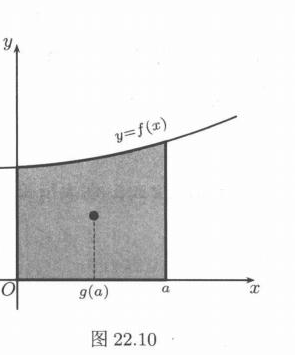
\includegraphics[width=.36\linewidth]{figures/lower/ch22/fig-22-10.png}
\end{center}
\[
  g(a)=\frac{M_x(1)}{M(0)}
  =\frac{\int_0^a x f(x)\,\dd x}{\int_0^a f(x)\,\dd x},
\]
即
\[
  g(a)\int_0^a f(x)\,\dd x=\int_0^a x f(x)\,\dd x.
\]
两边对 $a$ 求导得
\[
  g(a)f(a)+g'(a)\int_0^a f(x)\,\dd x=af(a).
\]
令 $F(a)=\int_0^a f(x)\,\dd x$，注意到 $a-g(a)\ne0$，则
\[
  \frac{F'(a)}{F(a)}=\frac{g'(a)}{a-g(a)}.
\]
两边对 $a$ 积分，得
\[
  \ln F(a)=\int\frac{g'(a)}{a-g(a)}\,\dd a+C.
\]
所以
\[
  \int_0^a f(x)\,\dd x=F(a)=A\exp\left(\int\frac{g'(a)}{a-g(a)}\,\dd a\right).
\]
两边对 $a$ 求导得
\[
  f(a)=\frac{Ag'(a)}{a-g(a)}\exp\left(\int\frac{g'(a)}{a-g(a)}\,\dd a\right).
\]
考虑到
\begin{align*}
  \int\frac{g'(a)}{a-g(a)}\,\dd a
  &=\int\frac{g'(a)-1}{a-g(a)}\,\dd a+\int\frac{\dd a}{a-g(a)}\\
  &=-\ln(a-g(a))+\int\frac{\dd a}{a-g(a)},
\end{align*}
则
\[
  f(a)=\frac{Ag'(a)}{[a-g(a)]^2}\exp\left(\int\frac{\dd a}{a-g(a)}\right).
\]
\end{xproof}

\textbf{引力}
考虑体密度函数为 $\mu(x,y,z)$ 的立体 $V$ 对具有质量 $m$ 的点 $p_0(x_0,y_0,z_0)$ 的引力 $\vect{F}$。由引力定律及微元法得 $\vect{F}=(F_x,F_y,F_z)$，其中
\[
  F_x=\iiint_V\frac{Gm\mu(x,y,z)(x-x_0)}{r^3}\,\dd x\,\dd y\,\dd z,
\]
\[
  F_y=\iiint_V\frac{Gm\mu(x,y,z)(y-y_0)}{r^3}\,\dd x\,\dd y\,\dd z,
\]
\[
  F_z=\iiint_V\frac{Gm\mu(x,y,z)(z-z_0)}{r^3}\,\dd x\,\dd y\,\dd z,
\]
其中 $G$ 为引力常量，$r=[(x-x_0)^2+(y-y_0)^2+(z-z_0)^2]^{1/2}$。

\subsection{重积分与不等式}

本段介绍重积分在不等式中的一些应用，先介绍如何用重积分的技巧证明一元的积分不等式。

\begin{xexample}[22.5.5]
设 $f$ 在 $[0,1]$ 上为正连续函数，证明：
\begin{equation}
  1\le\int_0^1\frac{\dd x}{f(x)}\int_0^1f(x)\,\dd x
  \le\frac{(m+M)^2}{4mM},
  \tag{22.10}
  \label{eq:22.10}
\end{equation}
其中 $m,M$ 分别为 $f(x)$ 在 $[0,1]$ 上的最小值和最大值（参见上册 374 页题 11）。
\end{xexample}
\begin{xproof}
设
\[
  I=\int_0^1\frac{\dd x}{f(x)}\int_0^1f(x)\,\dd x
  =\int_0^1\frac{\dd x}{f(x)}\int_0^1f(y)\,\dd y
  =\int_0^1\int_0^1\frac{f(y)}{f(x)}\,\dd x\,\dd y.
\]
由对称性
\[
  I=\frac12\int_0^1\int_0^1\left(\frac{f(y)}{f(x)}+\frac{f(x)}{f(y)}\right)\dd x\,\dd y.
\]
令 $F(z)=z+\frac1z,z>0$，则 $F(z)\ge2,F''(z)>0$，故 $F(z)$ 是凸函数。当 $F(\alpha)=F(\beta)$ 时，对 $z\in[\alpha,\beta]$ 有 $F(z)\le F(\alpha)=F(\beta)$。取 $z=\frac{f(y)}{f(x)},\alpha=\frac mM,\beta=\frac Mm$，得
\[
  2\le\frac{f(y)}{f(x)}+\frac{f(x)}{f(y)}\le\frac mM+\frac Mm,
\]
从而
\[
  1\le I\le\frac{m^2+M^2}{2mM}.
\]
但这与不等式 (22.10) 相比还不够精确。为此分析 (22.10)，由右端的平方启发用算术平均值—几何平均值不等式（上册第 4 页）得
\begin{equation}
  I=\int_0^1\frac{\dd x}{f(x)}\cdot\int_0^1f(x)\,\dd x
  \le\frac14\left[\int_0^1\left(f(x)+\frac1{f(x)}\right)\dd x\right]^2.
  \tag{22.11}
  \label{eq:22.11}
\end{equation}
但当 $m\le f(x)\le M$ 时不能充分利用 $z+\frac1z$ 的凸性来估计 $f(x)+\frac1{f(x)}$。观察 $I$ 的特点，用 $\frac{f(x)}{\sqrt{mM}}$ 替代 $f(x)$ 得
\[
  I=\int_0^1\frac{\sqrt{mM}}{f(x)}\,\dd x\cdot\int_0^1\frac{f(x)}{\sqrt{mM}}\,\dd x
  \le\frac14\left[\int_0^1\left(\frac{f(x)}{\sqrt{mM}}+\frac{\sqrt{mM}}{f(x)}\right)\dd x\right]^2.
\]
再取 $z=\frac{f(x)}{\sqrt{mM}},\alpha=\sqrt{\frac mM},\beta=\sqrt{\frac Mm}$，由 $z+\frac1z$ 的凸性得
\[
  I\le\frac14\left(\sqrt{\frac mM}+\sqrt{\frac Mm}\right)^2
  \le\frac{(m+M)^2}{4mM}.
\]
不等式 (22.10) 得证。
\end{xproof}

从上述证明过程可见，对学到的各种方法要善于比较，综合运用（本题还可参见上册 415 页的提示）。下面再举一个通过交换积分次序证明不等式的例子。

\begin{xexample}[22.5.6]
设 $f,\frac{\partial f}{\partial x},\frac{\partial f}{\partial t},\frac{\partial^2f}{\partial x^2}$ 均为 $[0,1]\times[0,1]$ 中的连续函数，且在 $[0,1]\times[0,1]$ 中成立
\[
  \frac{\partial f}{\partial t}=\frac{\partial^2f}{\partial x^2},
  \qquad
  \abs*{\frac{\partial f}{\partial x}}\le1.
\]
\begin{enumerate}[label=(\arabic*)]
  \item 证明：对任何 $(x,t_1),(x,t_2)\in[0,1]\times[0,1]$，存在 $\xi\in[0,1]$，使得 $\abs{\xi-x}\le\frac12\abs{t_1-t_2}^{1/2}$ 且
  \[
    \abs{f(\xi,t_1)-f(\xi,t_2)}\le4\abs{t_1-t_2}^{1/2};
  \]
  \item 由 (1) 的结论证明：对任何 $(x,t_1),(x,t_2)\in[0,1]\times[0,1]$ 成立
  \[
    \abs{f(x,t_1)-f(x,t_2)}\le5\abs{t_1-t_2}^{1/2}.
  \]
\end{enumerate}
\end{xexample}
\paragraph{分析}题目给出了 $f(x,t)$ 在 $x$ 方向上的性质：$\abs{\frac{\partial f}{\partial x}}\le1$。由此证明在 $t$ 方向上的性质。可用的条件是 $f$ 在 $x$ 方向和 $t$ 方向之间的关系：$\frac{\partial f}{\partial t}=\frac{\partial^2f}{\partial x^2}$。我们通过交换累次积分次序来转换。

\begin{xproof}
(1) 由题设
\[
  f(x,t_1)-f(x,t_2)=\int_{t_1}^{t_2}\frac{\partial f}{\partial t}(x,t)\,\dd t
  =\int_{t_1}^{t_2}\frac{\partial^2f}{\partial x^2}(x,t)\,\dd t.
\]
从而，对任何 $\bar x\in[0,1]$，由累次积分次序可交换，成立
\begin{align*}
  \int_{\bar x}^x[f(x,t_1)-f(x,t_2)]\,\dd x
  &=\int_{\bar x}^x\left(\int_{t_1}^{t_2}\frac{\partial^2f}{\partial x^2}(x,t)\,\dd t\right)\dd x\\
  &=\int_{t_1}^{t_2}\left(\int_{\bar x}^x\frac{\partial^2f}{\partial x^2}(x,t)\,\dd x\right)\dd t\\
  &=\int_{t_1}^{t_2}\left(\frac{\partial f}{\partial x}(x,t)-\frac{\partial f}{\partial x}(\bar x,t)\right)\dd t.
\end{align*}
对上式左端应用积分中值定理，右端利用已知条件 $\abs{\frac{\partial f}{\partial x}}\le1$，得
\[
  \abs{f(\xi,t_1)-f(\xi,t_2)}\cdot\abs{x-\bar x}\le2\abs{t_1-t_2},
\]
其中 $\xi$ 在 $x$ 和 $\bar x$ 之间。对任何 $x,t_1,t_2\in[0,1]$ 总可找到某个 $\bar x\in[0,1]$，使得
\[
  \abs{x-\bar x}=\frac12\abs{t_1-t_2}^{1/2},
\]
代入前式即得
\[
  \abs{f(\xi,t_1)-f(\xi,t_2)}\le4\abs{t_1-t_2}^{1/2}.
\]

(2) 利用 (1) 得
\begin{align*}
  \abs{f(x,t_1)-f(x,t_2)}
  &\le\abs{f(x,t_1)-f(\xi,t_1)}+\abs{f(\xi,t_1)-f(\xi,t_2)}+\abs{f(x,t_2)-f(\xi,t_2)}\\
  &\le1\cdot\abs{x-\xi}+4\abs{t_1-t_2}^{1/2}+1\cdot\abs{x-\xi}\\
  &\le\abs{x-\bar x}+4\abs{t_1-t_2}^{1/2}+\abs{x-\bar x}
  =5\abs{t_1-t_2}^{1/2}.
\end{align*}
\end{xproof}

最后，我们证明重积分形式的 Hölder 不等式，并由此推出一些有用的估计。

设 $\Omega$ 是 $\RR^2$ 中可求面积的有界区域，函数 $f$ 定义在 $\Omega$ 上，如果 $\abs{f}^p$（$p>0$）在 $\Omega$ 上广义可积，则称 $f$ 是在 $\Omega$ 上 $p$ 次（广义）可积。$\Omega$ 上的 $p$ 次可积函数的全体记为 $L^p(\Omega)$，且记
\[
  \norm{f}_p=\left(\iint_\Omega\abs{f(x,y)}^p\,\dd x\,\dd y\right)^{1/p}.
\]

\begin{xexample}[22.5.7（Hölder 不等式）]
设 $u\in L^p(\Omega),v\in L^q(\Omega),p,q>1$，且 $\frac1p+\frac1q=1$，则
\[
  \norm{uv}_1\le\norm{u}_p\norm{v}_q.
\]
\end{xexample}
\begin{xproof}
不妨设 $\norm{u}_p>0,\norm{v}_q>0$。令
\[
  a=\frac{\abs{u}}{\norm{u}_p},\qquad b=\frac{\abs{v}}{\norm{v}_q}.
\]
由 Young 不等式（上册 259 页题 10）：
\[
  ab\le\frac{a^p}{p}+\frac{b^q}{q},
\]
其中 $p,q>1,\frac1p+\frac1q=1,a,b\ge0$，得到
\[
  \frac{\abs{u}\cdot\abs{v}}{\norm{u}_p\norm{v}_q}
  \le\frac{\abs{u}^p}{p\norm{u}_p^p}+\frac{\abs{v}^q}{q\norm{v}_q^q}.
\]
两边在 $\Omega$ 上积分得
\[
  \frac{\iint_\Omega\abs{u}\cdot\abs{v}\,\dd x\,\dd y}{\norm{u}_p\norm{v}_q}
  \le\frac1p+\frac1q=1.
\]
由此得出所要证明的不等式（参见上册 349--350 页）。
\end{xproof}

\begin{xexample}[22.5.8]
设 $u\in L^q(\Omega),0<p\le q$，则
\[
  \abs{\Omega}^{-1/p}\norm{u}_p\le\abs{\Omega}^{-1/q}\norm{u}_q,
\]
其中 $\abs{\Omega}$ 表示 $\Omega$ 的体积。
\end{xexample}
\begin{xproof}
由 Hölder 不等式
\begin{align*}
  \norm{u}_p^p=\iint_\Omega\abs{u}^p\,\dd x\,\dd y
  &\le\left[\iint_\Omega(\abs{u}^p)^{q/p}\,\dd x\,\dd y\right]^{p/q}
  \left[\iint_\Omega1^{q/(q-p)}\,\dd x\,\dd y\right]^{(q-p)/q}\\
  &=\abs{\Omega}^{(q-p)/q}\norm{u}_q^p.
\end{align*}
两边开 $p$ 次方，则
\[
  \norm{u}_p\le\abs{\Omega}^{1/p-1/q}\norm{u}_q.
\]
\end{xproof}

\begin{xremark}
由上例的结论知对任意 $0<p\le q$，$L^q(\Omega)\subset L^p(\Omega)$。
\end{xremark}

\begin{xexample}[22.5.9]
设 $u\in L^r(\Omega),0<p\le q\le r$，则
\[
  \norm{u}_q\le\norm{u}_p^\lambda\norm{u}_r^{1-\lambda},
\]
其中 $\lambda$ 满足
\[
  \frac1q=\frac\lambda p+\frac{1-\lambda}{r}.
\]
\end{xexample}
\begin{xproof}
由 Hölder 不等式
\begin{align*}
  \norm{u}_q^q
  &=\iint_\Omega\abs{u}^q\,\dd x\,\dd y
  =\iint_\Omega\abs{u}^{\lambda q}\abs{u}^{(1-\lambda)q}\,\dd x\,\dd y\\
  &\le\left[\iint_\Omega(\abs{u}^{\lambda q})^{p/(\lambda q)}\,\dd x\,\dd y\right]^{\lambda q/p}
  \left[\iint_\Omega(\abs{u}^{(1-\lambda)q})^{r/((1-\lambda)q)}\,\dd x\,\dd y\right]^{(1-\lambda)q/r}\\
  &=\norm{u}_p^{\lambda q}\norm{u}_r^{(1-\lambda)q}.
\end{align*}
两边开 $q$ 次方即为所求。
\end{xproof}

\begin{xexample}[22.5.10]
设 $u,u_x,u_y$ 在有界区域 $\Omega\subset\RR^2$ 上连续，且在 $\Omega$ 的边界 $\partial\Omega$ 上 $u=u_x=u_y=0$，则对于 $1\le p<2$ 有
\[
  \norm{u}_{\frac{2p}{2-p}}\le C(\norm{u_x}_p+\norm{u_y}_p),
\]
其中 $C$ 只与 $p$ 有关，与 $u$ 无关。
\end{xexample}
\begin{xproof}
先设 $p=1$。当 $(x,y)\in\RR^2\setminus\Omega$ 时，定义 $u(x,y)=0$，则
\[
  u(x,y)=\int_{-\infty}^x u_x(x,y)\,\dd x,
  \qquad
  u(x,y)=\int_{-\infty}^y u_y(x,y)\,\dd y.
\]
从而
\[
  \abs{u(x,y)}\le\int_{-\infty}^x\abs{u_x}\,\dd x,
  \qquad
  \abs{u(x,y)}\le\int_{-\infty}^y\abs{u_y}\,\dd y.
\]
由此得
\[
  \abs{u(x,y)}^2\le\int_{-\infty}^{+\infty}\abs{u_x(x,y)}\,\dd x
  \int_{-\infty}^{+\infty}\abs{u_y(x,y)}\,\dd y.
\]
两边在 $\RR^2$ 上积分得到
\[
  \iint_\Omega\abs{u(x,y)}^2\,\dd x\,\dd y
  \le\iint_\Omega\abs{u_x}\,\dd x\,\dd y\iint_\Omega\abs{u_y}\,\dd x\,\dd y.
\]
两边开平方，得
\[
  \norm{u}_2\le\norm{u_x}_1^{1/2}\norm{u_y}_1^{1/2}.
\]
利用 $\sqrt{ab}\le\frac12(a+b)$，就有
\begin{equation}
  \norm{u}_2\le\frac12(\norm{u_x}_1+\norm{u_y}_1).
  \tag{22.12}
  \label{eq:22.12}
\end{equation}
这就证明了 $p=1$ 时的结论。

当 $1<p<2$ 时，令 $\gamma=\frac p{2-p}$，在 (22.12) 中用 $u^\gamma$ 代替 $u$，则
\begin{align}
  \norm{u^\gamma}_2
  &\le\frac12(\norm{\gamma u^{\gamma-1}u_x}_1+\norm{\gamma u^{\gamma-1}u_y}_1)\notag\\
  &\le\frac\gamma2(\norm{u^{\gamma-1}}_q\norm{u_x}_p+\norm{u^{\gamma-1}}_q\norm{u_y}_p),
  \tag{22.13}
  \label{eq:22.13}
\end{align}
其中 $q$ 满足 $\frac1p+\frac1q=1$，即 $q=\frac p{p-1}$。由于
\[
  \norm{u^\gamma}_2=\norm{u}_{2\gamma}^\gamma=\norm{u}_{\frac{2p}{2-p}}^\gamma,
\]
\[
  \norm{u^{\gamma-1}}_q=\norm{u}_{(\gamma-1)q}^{\gamma-1}
  =\norm{u}_{\frac{2p}{2-p}}^{\gamma-1},
\]
由 (22.13) 得
\[
  \norm{u}_{\frac{2p}{2-p}}\le\frac\gamma2(\norm{u_x}_p+\norm{u_y}_p).
\]
\end{xproof}

\subsection{练习题}

\begin{xexercise}[1]
计算由下列曲面围成的立体体积：
  \begin{enumerate}[label=(\arabic*)]
    \item $a_ix+b_iy+c_iz=\pm h_i$，$i=1,2,3$，其中三个平面的法向线性无关；
    \item $(x^2+y^2+z^2)^2=a^3z$，其中 $a>0$；
    \item $\displaystyle\left(\frac{x^2}{a^2}+\frac{y^2}{b^2}+\frac{z^2}{c^2}\right)^2=\frac{x^2}{a^2}+\frac{y^2}{b^2}$；
    \item $(x^2+y^2)^2+z^4=z$。
  \end{enumerate}
\end{xexercise}
\begin{xsolution}
\begin{enumerate}[label=(\arabic*)]
  \item 记
  \[
   \Delta=\det
   \begin{pmatrix}
    a_1&b_1&c_1\\
    a_2&b_2&c_2\\
    a_3&b_3&c_3
   \end{pmatrix}\ne0.
  \]
  作线性变换
  \[
   u_i=a_ix+b_iy+c_iz,
   \qquad i=1,2,3.
  \]
  原立体变为长方体 $\abs{u_i}\le h_i$，并且
  \[
   \dd x\,\dd y\,\dd z=\frac1{\abs\Delta}\,\dd u_1\,\dd u_2\,\dd u_3.
  \]
  故体积
  \[
   \boxed{V=\frac{8h_1h_2h_3}{\abs\Delta}}.
  \]

  \item 用球坐标 $z=r\cos\varphi$。曲面方程化为
  \[
   r^4=a^3r\cos\varphi,
   \qquad r^3=a^3\cos\varphi.
  \]
  因而 $0\le\varphi\le\pi/2$，$0\le r\le a(\cos\varphi)^{1/3}$。于是
  \begin{align*}
   V&=\int_0^{2\pi}\int_0^{\pi/2}\int_0^{a(\cos\varphi)^{1/3}}
   r^2\sin\varphi\,\dd r\,\dd\varphi\,\dd\theta\\
   &=\frac{2\pi a^3}{3}\int_0^{\pi/2}\cos\varphi\sin\varphi\,\dd\varphi
   =\boxed{\frac{\pi a^3}{3}}.
  \end{align*}

  \item 令
  \[
   X=\frac xa,
   \qquad Y=\frac yb,
   \qquad Z=\frac zc.
  \]
  则体积乘上因子 $abc$，而边界变为
  \[
   (X^2+Y^2+Z^2)^2=X^2+Y^2.
  \]
  在球坐标中为 $r^2=\sin^2\varphi$，即 $0\le r\le\sin\varphi$。故
  \begin{align*}
   V&=abc\int_0^{2\pi}\int_0^\pi\int_0^{\sin\varphi}
   r^2\sin\varphi\,\dd r\,\dd\varphi\,\dd\theta\\
   &=\frac{2\pi abc}{3}\int_0^\pi\sin^4\varphi\,\dd\varphi
   =\boxed{\frac{\pi^2abc}{4}}.
  \end{align*}

  \item 采用柱坐标。由
  \[
   r^4+z^4=z
  \]
  知 $0\le z\le1$，且
  \[
   0\le r\le(z-z^4)^{1/4}.
  \]
  因而
  \begin{align*}
   V&=\pi\int_0^1\sqrt{z-z^4}\,\dd z
   =\pi\int_0^1z^{1/2}(1-z^3)^{1/2}\,\dd z\\
   &=\frac\pi3\int_0^1u^{-1/2}(1-u)^{1/2}\,\dd u
   \qquad(u=z^3)\\
   &=\frac{2\pi}{3}\int_0^{\pi/2}\cos^2 t\,\dd t
   \qquad(u=\sin^2t)\\
   &=\boxed{\frac{\pi^2}{6}}.
  \end{align*}
\end{enumerate}
\end{xsolution}


\begin{xexercise}[2]
计算下列曲面的面积：
  \begin{enumerate}[label=(\arabic*)]
    \item $(x^2+y^2+z^2)^2=x^2-y^2$；
    \item $(x^2+y^2+z^2)^2=z^3$；
    \item 连续曲线 $y=f(x)$（$\ge0$），$x\in[a,b]$，绕 $x$ 轴旋转所得曲面。
  \end{enumerate}
\end{xexercise}
\begin{xsolution}
\begin{enumerate}[label=(\arabic*)]
  \item 在球坐标中，曲面写成
  \[
   r=R(\varphi,\theta)=\sin\varphi\sqrt{\cos2\theta},
  \]
  其中 $0\le\varphi\le\pi$，而 $\cos2\theta\ge0$，即
  \[
   \theta\in\left[-\frac\pi4,\frac\pi4\right]
   \cup\left[\frac{3\pi}{4},\frac{5\pi}{4}\right].
  \]
  对球坐标中的径向图 $r=R(\varphi,\theta)$，
  \[
   \dd S=R^2\sin\varphi
   \sqrt{1+\left(\frac{R_\varphi}{R}\right)^2+
   \left(\frac{R_\theta}{R\sin\varphi}\right)^2}
   \,\dd\varphi\,\dd\theta.
  \]
  此处
  \[
   \frac{R_\varphi}{R}=\cot\varphi,
   \qquad
   \frac{R_\theta}{R}=-\tan2\theta,
  \]
  所以在 $\cos2\theta>0$ 的区域内恰有
  \[
   \dd S=\sin^2\varphi\,\dd\varphi\,\dd\theta.
  \]
  两个 $\theta$ 区间的总长度为 $\pi$，故
  \[
   \boxed{S=\pi\int_0^\pi\sin^2\varphi\,\dd\varphi=\frac{\pi^2}{2}}.
  \]

  \item 球坐标下方程为
  \[
   r^4=(r\cos\varphi)^3,
   \qquad r=\cos^3\varphi,
  \]
  因而 $0\le\varphi\le\pi/2$。径向图面积元为
  \[
   \dd S=\cos^5\varphi\sin\varphi
   \sqrt{\cos^2\varphi+9\sin^2\varphi}
   \,\dd\varphi\,\dd\theta.
  \]
  令 $s=\cos\varphi$，得
  \begin{align*}
   S&=2\pi\int_0^1s^5\sqrt{9-8s^2}\,\dd s
   =\boxed{\frac{313\pi}{560}}.
  \end{align*}

  \item 若母线以弧长 $s$ 为参数，则旋转面面积微元为 $2\pi y\,\dd s$，所以
  \[
   \boxed{S=2\pi\int_\Gamma y\,\dd s}.
  \]
  若进一步 $f\in C^1[a,b]$，则 $\dd s=\sqrt{1+[f'(x)]^2}\,\dd x$，从而
  \[
   \boxed{S=2\pi\int_a^bf(x)\sqrt{1+[f'(x)]^2}\,\dd x}.
  \]
\end{enumerate}
\end{xsolution}


\begin{xexercise}[3]
设抛物面壳 $z=\frac12(x^2+y^2)$（$0\le z\le1$）的面密度 $\rho=z$，求质量。
\end{xexercise}
\begin{xsolution}
抛物面写成
\[
 z=\frac12r^2,
 \qquad0\le r\le\sqrt2.
\]
其面积元为
\[
 \dd S=\sqrt{1+z_x^2+z_y^2}\,\dd x\,\dd y
 =\sqrt{1+r^2}\,r\,\dd r\,\dd\theta.
\]
面密度 $\rho=z=r^2/2$，故质量
\begin{align*}
 m&=\int_0^{2\pi}\int_0^{\sqrt2}
 \frac{r^2}{2}\sqrt{1+r^2}\,r\,\dd r\,\dd\theta\\
 &=\pi\int_0^{\sqrt2}r^3\sqrt{1+r^2}\,\dd r
 =\boxed{\frac{2\pi}{15}(6\sqrt3+1)}.
\end{align*}
\end{xsolution}


\begin{xexercise}[4]
半径为 $R$ 的均匀圆盘，其密度为 $\mu$。过圆心且与圆垂直的直线上有一密度为 $\rho$ 的均匀细棒，棒长为 $l$，其近圆盘的一端与圆心相距为 $a$。求圆盘对细棒的引力。
\end{xexercise}
\begin{xsolution}
取圆盘中心为原点，细棒沿 $z$ 轴，近端为 $z=a$，远端为 $z=a+l$。圆盘面密度为 $\mu$。位于轴上距离圆盘为 $z>0$ 的单位质量所受引力大小为
\begin{align*}
 g(z)&=\int_0^R\frac{G\mu z}{(r^2+z^2)^{3/2}}\,2\pi r\,\dd r\\
 &=2\pi G\mu\left(1-\frac{z}{\sqrt{z^2+R^2}}\right).
\end{align*}
细棒线密度为 $\rho$，所以圆盘对整根细棒的引力大小为
\begin{align*}
 F&=\rho\int_a^{a+l}g(z)\,\dd z\\
 &=2\pi G\mu\rho
 \left[z-\sqrt{z^2+R^2}\right]_{a}^{a+l}\\
 &=\boxed{2\pi G\mu\rho
 \left(l+\sqrt{a^2+R^2}-\sqrt{(a+l)^2+R^2}\right)}.
\end{align*}
方向沿细棒指向圆盘。
\end{xsolution}


\begin{xexercise}[5]
半径为 $a$ 的圆盘，其各点的密度等于该点到圆心的距离。今从圆盘上挖去一个半径为 $\frac a2$ 而其圆心离圆盘中心为 $\frac a2$ 的小圆盘。求剩下几何图形的重心坐标。
\end{xexercise}
\begin{xsolution}
取大圆盘中心为原点，小圆盘中心在 $(a/2,0)$；若小圆盘位于其他方向，最后把坐标轴旋转即可。原大圆盘的密度为到原点的距离 $r$，故总质量
\[
 M_0=\int_0^{2\pi}\int_0^a r\cdot r\,\dd r\,\dd\theta
 =\frac{2\pi a^3}{3},
\]
且重心在原点。

被挖去的小圆盘在原点极坐标中为
\[
 -\frac\pi2\le\theta\le\frac\pi2,
 \qquad0\le r\le a\cos\theta.
\]
其质量为
\[
 M_1=\int_{-\pi/2}^{\pi/2}\int_0^{a\cos\theta}r^2\,\dd r\,\dd\theta
 =\frac{4a^3}{9}.
\]
它关于 $y$ 轴的一阶矩为
\[
 Q_{y,1}=\int_{-\pi/2}^{\pi/2}\int_0^{a\cos\theta}
 (r\cos\theta)r^2\,\dd r\,\dd\theta
 =\frac{4a^4}{15},
\]
而关于 $x$ 轴的一阶矩为零。剩余部分的质量及一阶矩因此为
\[
 M=M_0-M_1=\frac{2a^3}{9}(3\pi-2),
 \qquad Q_y=-\frac{4a^4}{15},
 \qquad Q_x=0.
\]
所以重心坐标为
\[
 \boxed{
 \left(\bar x,\bar y\right)
 =\left(-\frac{6a}{5(3\pi-2)},0\right)}.
\]
若小圆盘中心沿单位向量 $\vect e$，则重心向量为
$-\dfrac{6a}{5(3\pi-2)}\vect e$。
\end{xsolution}


\begin{xexercise}[6]
假定物体有连续的密度函数，证明：凸形物体的重心必在其体内。
\end{xexercise}
\begin{xsolution}
设凸形物体为紧凸集 $K\subset\RR^3$，连续密度 $\rho\ge0$，总质量
\[
 m=\iiint_K\rho\,\dd V>0,
\]
重心为
\[
 C=\frac1m\iiint_K\vect x\,\rho(\vect x)\,\dd V.
\]
若 $C\notin K$，由凸集分离定理，存在向量 $\vect n$ 与常数 $\alpha$，使
\[
 \vect n\cdot C>\alpha\ge\vect n\cdot\vect x,
 \qquad\forall\vect x\in K.
\]
但由重心定义
\[
 \vect n\cdot C
 =\frac1m\iiint_K(\vect n\cdot\vect x)\rho(\vect x)\,\dd V
 \le\alpha,
\]
矛盾。因此 $C\in K$。

事实上，由 $m>0$ 与 $\rho\ge0$ 的连续性，存在物体内的一个相对开集使 $\rho>0$。若 $C$ 位于边界支撑平面 $\vect n\cdot\vect x=\alpha$ 上，则物体内有 $\vect n\cdot\vect x\le\alpha$，并在上述正密度开集的一部分上严格小于 $\alpha$，从而
\[
  \vect n\cdot C
  =\frac1m\iiint_K(\vect n\cdot\vect x)\rho(\vect x)\,\dd V<\alpha,
\]
与 $C$ 在该支撑平面上矛盾。因此 $C$ 不在边界上，故重心位于凸形物体内部。
\end{xsolution}


\begin{xexercise}[7]
设 $u_i\in L^{p_i}(\Omega),p_i>0,i=1,2,\ldots,m$，且 $\sum_{i=1}^m\frac1{p_i}=1$。证明：
  \[
    \iint_\Omega u_1u_2\cdots u_m\,\dd x\,\dd y
    \le\norm{u_1}_{p_1}\norm{u_2}_{p_2}\cdots\norm{u_m}_{p_m}.
  \]
\end{xexercise}
\begin{xsolution}
对因子个数 $m$ 作归纳。$m=1$ 时由 $1/p_1=1$ 得 $p_1=1$，结论即为等式；$m=2$ 时就是 Hölder 不等式。

设结论对 $m-1$ 个因子成立，现考虑 $m\ge3$。令
\[
 \frac1r=\frac1{p_{m-1}}+\frac1{p_m}.
\]
由于
\[
 \sum_{i=1}^{m-2}\frac1{p_i}+\frac1r=1,
\]
有 $r>1$。又
\[
 \frac{r}{p_{m-1}}+\frac{r}{p_m}=1,
\]
故对 $u_{m-1},u_m$ 应用 Hölder 不等式可得
\begin{align*}
 \norm{u_{m-1}u_m}_r^r
 &=\iint_\Omega\abs{u_{m-1}}^r\abs{u_m}^r\,\dd x\,\dd y\\
 &\le
 \left(\iint_\Omega\abs{u_{m-1}}^{p_{m-1}}\,\dd x\,\dd y\right)^{r/p_{m-1}}
 \left(\iint_\Omega\abs{u_m}^{p_m}\,\dd x\,\dd y\right)^{r/p_m}.
\end{align*}
因此
\[
 \norm{u_{m-1}u_m}_r
 \le\norm{u_{m-1}}_{p_{m-1}}\norm{u_m}_{p_m}.
\]
再对 $m-1$ 个因子
\[
 u_1,\ldots,u_{m-2},u_{m-1}u_m
\]
以及指数 $p_1,\ldots,p_{m-2},r$ 使用归纳假设，得到
\begin{align*}
 \abs*{\iint_\Omega u_1u_2\cdots u_m\,\dd x\,\dd y}
 &\le\norm{u_1}_{p_1}\cdots\norm{u_{m-2}}_{p_{m-2}}
 \norm{u_{m-1}u_m}_r\\
 &\le\norm{u_1}_{p_1}\norm{u_2}_{p_2}\cdots\norm{u_m}_{p_m}.
\end{align*}
因此题中不带绝对值的积分当然也满足所给上界。
\end{xsolution}


\begin{xexercise}[8]
证明：
  \[
    \left\{\int_a^b\dd x\left[\int_c^d f(x,y)\,\dd y\right]^2\right\}^{1/2}
    \le\int_c^d\dd y\left[\int_a^b f^2(x,y)\,\dd x\right]^{1/2},
  \]
  其中 $f$ 是连续函数。
\end{xexercise}
\begin{xsolution}
令
\[
 F(x)=\int_c^df(x,y)\,\dd y.
\]
则由 Fubini 交换积分次序以及关于 $x$ 的 Cauchy--Schwarz 不等式，
\begin{align*}
 \int_a^bF^2(x)\,\dd x
 &=\int_c^d\int_c^d
 \left(\int_a^bf(x,y)f(x,z)\,\dd x\right)\dd y\,\dd z\\
 &\le\int_c^d\int_c^d
 \left(\int_a^bf^2(x,y)\,\dd x\right)^{1/2}
 \left(\int_a^bf^2(x,z)\,\dd x\right)^{1/2}
 \dd y\,\dd z\\
 &=\left[
 \int_c^d\left(\int_a^bf^2(x,y)\,\dd x\right)^{1/2}\dd y
 \right]^2.
\end{align*}
两边开平方即得所要求的不等式。
\end{xsolution}


\section{对于教学的建议}

\subsection{学习要点}

1. 如何快速准确计算出重积分的值是本章的重点之一。为此有三点是至关重要的：一是选择坐标变换，二是选择积分顺序，三是要优先利用对称性，即积分区域的对称性与被积函数的奇偶性。

2. 计算重积分的过程中，画出积分区域的示意图是很重要的一个步骤。示意图的要点是区域所处的象限（或卦限）、曲线的交点（曲面的交线）。用球坐标时尤其要准确标出交线。即使画不出图，也要作必要的几何分析。例如对 $(x^2+y^2)^2+z^4=z$ 所围立体，首先从方程看出立体位于平面 $z=0$ 和 $z=1$ 之间，其次可看出这是一个旋转面，令 $y=0$ 得母线 $x^4=z-z^4$。

3. 要充分重视重积分的应用部分的教学。这里微元法是个重点。要注意微元法的“求和”并不是简单的相加。在“曲”的坐标下考虑的是求和方向上的分量相加。比如求移动曲面扫过的体积，我们必须考虑移动的法向速度方向上的求和。

4. 重积分的计算是熟能生巧，需要做大量的习题。限于篇幅，我们仅仅列举一些有特点的例子。在一般的教科书上（如 [24]）都给出了足够丰富的例题与习题。请读者自己把握。还可以参考 [25,55] 第八章的前 10 节。

5. \textbf{对习题课的建议}
应该根据实际需要选择坐标变换，不能只会一种。任何一种坐标变换都不是万能的。球坐标变换很重要，但并不是积分区域与球有关就要用球坐标。如例题 22.3.1，用球坐标就不简单。

关于积分顺序，应该观察被积函数与积分区域两者的特点，尽可能使积分变得简单。仍考察例题 22.3.1，被积函数中有 $z$，当然应该选择“先二后一”的顺序，而且是先对 $x,y$，后对 $z$，这样对 $x,y$ 作二重积分时，被积函数是常数，因而可以提到积分号之外。

对称性的使用不仅可以简化计算，还有助于避免错误。下面的例子可以很清楚地说明这一点。

\begin{xexample}[22.6.1]
求球体 $x^2+y^2+z^2\le a^2$ 和圆柱体 $x^2+y^2\le ax$（$a>0$）的公共部分所成的空间区域（Viviani（维维亚尼）体）的体积 $V$。
\end{xexample}
\begin{xsolution}
如图 22.11（半个 Viviani 体）所示，
\begin{center}
  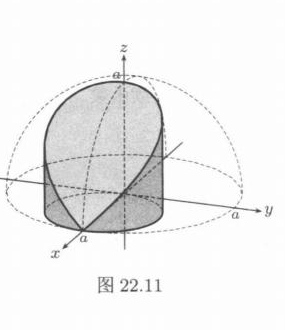
\includegraphics[width=.36\linewidth]{figures/lower/ch22/fig-22-11.png}
\end{center}
\begin{align*}
  V&=2\iint_{x^2+y^2\le ax}\sqrt{a^2-x^2-y^2}\,\dd x\,\dd y\\
  &=2\int_{-\pi/2}^{\pi/2}\dd\theta\int_0^{a\cos\theta}r\sqrt{a^2-r^2}\,\dd r\\
  &=\int_{-\pi/2}^{\pi/2}-\frac23(a^2-r^2)^{3/2}\bigg|_0^{a\cos\theta}\,\dd\theta\\
  &=-\frac23\int_{-\pi/2}^{\pi/2}\left[(a^2\sin^2\theta)^{3/2}-a^3\right]\dd\theta.
\end{align*}
再往下作就有两种可能了，一种是
\[
  (\sin^2\theta)^{3/2}=\sin^3\theta\quad\text{（这是错的！）},
\]
应该是
\[
  (\sin^2\theta)^{3/2}=\abs{\sin\theta}^3.
\]
但如果一开始就利用对称性，得
\[
  V=4\iint_{\substack{x^2+y^2\le ax\\y\ge0}}\sqrt{a^2-x^2-y^2}\,\dd x\,\dd y,
\]
不但使运算简便，而且无形中避免了上述错误的发生。
\end{xsolution}

\subsection{参考题}

\subsubsection*{第一组参考题}

\begin{xreferenceproblem}[1]
设 $f(x,y)$ 在 $D=\{(x,y)\mid0\le x\le1,0\le y\le1\}$ 上有如下定义：
  \[
    f(x,y)=
    \begin{cases}
      \dfrac1{q_x}, & \text{当 }x=\dfrac{p_x}{q_x},\ y\text{ 是无理数时},\\
      \dfrac1{q_y}, & \text{当 }y=\dfrac{p_y}{q_y},\ x\text{ 是无理数时},\\
      0, & \text{其他情况},
    \end{cases}
  \]
  其中 $q_x,q_y$ 分别表示有理数 $x,y$ 写成既约分数后的分母。则 $f(x,y)$ 在 $D$ 上可积，但两个二次积分不存在。
\end{xreferenceproblem}
\begin{xsolution}
先考察可积性。若 $(x_0,y_0)$ 的两个坐标都是无理数，则对任意 $N\in\NN$，可以取其充分小的邻域，使其中所有分母不超过 $N$ 的有理数都避开 $x_0,y_0$。于是该邻域内
\[
  0\le f(x,y)\le\frac1N,
\]
故 $f$ 在 $(x_0,y_0)$ 连续且值为 $0$。

因此 $f$ 的不连续点只能落在
\[
  \bigl((\QQ\cap[0,1])\times[0,1]\bigr)
  \cup
  \bigl([0,1]\times(\QQ\cap[0,1])\bigr),
\]
这是可列条直线之并，是零测度集。函数又有界，故由可积判别准则，$f$ 在 $D$ 上可积。并且连续点处函数值均为 $0$，由例题 22.1.2 的结论
\[
  \iint_Df(x,y)\,\dd x\,\dd y=0.
\]

下面说明两个二次积分均不存在。固定一个有理数 $y=p_y/q_y$。当 $x$ 为无理数时，
\[
  f(x,y)=\frac1{q_y},
\]
而当 $x$ 为有理数时 $f(x,y)=0$。因此 $x\mapsto f(x,y)$ 在 $[0,1]$ 上处处不连续，故
\[
  \int_0^1f(x,y)\,\dd x
\]
不存在。于是先对 $x$ 积分的二次积分不存在。同理，固定任一有理数 $x$，$y\mapsto f(x,y)$ 也处处不连续，所以先对 $y$ 积分的二次积分也不存在。
\end{xsolution}


\begin{xreferenceproblem}[2]
设 $f(x,y)$ 定义在 $D=\{(x,y)\mid0\le x\le1,0\le y\le1\}$ 上，
  \[
    f(x,y)=
    \begin{cases}
      1, & \text{当 }x\text{ 和 }y\text{ 都是非零有理数，}x=\dfrac{p_x}{q_x},y=\dfrac{p_y}{q_y}\text{ 且 }q_x=q_y\text{ 时},\\
      0, & \text{其他情况},
    \end{cases}
  \]
  其中 $q_x,q_y$ 表示有理数 $x,y$ 写成既约分数后的分母。证明 $f(x,y)$ 在 $D$ 上不可积，但两个二次积分存在且相等。
\end{xreferenceproblem}
\begin{xsolution}
先考察截面。固定 $y\in[0,1]$。若 $y$ 是无理数或 $y=0$，则除至多有限情形外截面函数恒为 $0$；若 $y=p_y/q_y\ne0$ 为既约有理数，则
\[
  f(x,y)=1
\]
只可能发生在 $x$ 是分母同为 $q_y$ 的既约有理数时。这样的 $x\in[0,1]$ 只有有限个。因此对每个固定的 $y$，$x\mapsto f(x,y)$ 都只在有限点取 $1$，其余处取 $0$，故可积且积分为 $0$。于是
\[
  \int_0^1\dd y\int_0^1f(x,y)\,\dd x=0.
\]
完全同理，另一二次积分也存在且为 $0$。

但 $f$ 在 $D$ 的每一点都不连续。事实上，$f=0$ 的点在 $D$ 中稠密，例如至少有一个坐标为无理数的点构成稠密集。另一方面，$f=1$ 的点也稠密：给定任意 $(x_0,y_0)$ 和任意邻域，取充分大的素数 $q$，可以分别选取整数 $p_1,p_2$，使 $p_i/q$ 落在对应坐标的小邻域内；由于 $q$ 为素数并可避开端点，两个分数可取为既约分数且分母同为 $q$，故此点处 $f=1$。于是任一点的任意邻域内同时有函数值 $0$ 和 $1$，所以 $f$ 处处不连续。其不连续点集为整个正方形，非零测度，因此 $f$ 在 $D$ 上不可积。
\end{xsolution}


\begin{xreferenceproblem}[3]
\begin{enumerate}[label=(\arabic*)]
    \item 计算积分 $\displaystyle A=\int_0^1\int_0^1\abs*{xy-\frac14}\,\dd x\,\dd y$；
    \item 设 $z=f(x,y)$ 在闭正方形 $D=\{(x,y)\mid0\le x\le1,0\le y\le1\}$ 上连续，且满足下列条件：
    \[
      \iint_D f(x,y)\,\dd x\,\dd y=0,
      \qquad
      \iint_D xyf(x,y)\,\dd x\,\dd y=1.
    \]
    求证：$\exists(\xi,\eta)\in D$ 使得 $\abs{f(\xi,\eta)}\ge\dfrac1A$。
  \end{enumerate}
\end{xreferenceproblem}
\begin{xsolution}
\begin{enumerate}[label=(\arabic*)]
  \item 固定 $x$。当 $0\le x\le1/4$ 时，$xy\le1/4$ 对所有 $0\le y\le1$ 成立；当 $1/4<x\le1$ 时，变号点为 $y=1/(4x)$。故
  \begin{align*}
    A&=\int_0^{1/4}\int_0^1\left(\frac14-xy\right)\dd y\,\dd x\\
     &\quad+\int_{1/4}^1\left[
      \int_0^{1/(4x)}\left(\frac14-xy\right)\dd y
      +\int_{1/(4x)}^1\left(xy-\frac14\right)\dd y
    \right]\dd x\\
    &=\boxed{\frac3{32}+\frac18\ln2}.
  \end{align*}

  \item 由题设两式相减，
  \[
    \iint_D\left(xy-\frac14\right)f(x,y)\,\dd x\,\dd y=1.
  \]
  设
  \[
    M=\max_{(x,y)\in D}\abs{f(x,y)}.
  \]
  则
  \[
    1\le M\iint_D\abs*{xy-\frac14}\,\dd x\,\dd y=MA.
  \]
  因而 $M\ge1/A$。由于连续函数在紧集 $D$ 上达到最大绝对值，存在 $(\xi,\eta)\in D$ 使
  \[
    \boxed{\abs{f(\xi,\eta)}\ge\frac1A}.
  \]
\end{enumerate}
\end{xsolution}


\begin{xreferenceproblem}[4]
证明：
  \[
    1.96<\iint_{\abs{x}+\abs{y}\le10}\frac1{100+\cos^2x+\cos^2y}\,\dd x\,\dd y<2.
  \]
\end{xreferenceproblem}
\begin{xsolution}
区域 $\abs{x}+\abs{y}\le10$ 是两条对角线均为 $20$ 的菱形，面积为
\[
  \abs{D}=200.
\]
又
\[
  100<100+\cos^2x+\cos^2y\le102
\]
除去零面积的特殊点外均严格成立相应的一侧，因此
\[
  \frac{200}{102}<
  \iint_D\frac{\dd x\,\dd y}{100+\cos^2x+\cos^2y}
  <\frac{200}{100}.
\]
由于
\[
  \frac{200}{102}=\frac{100}{51}>\frac{49}{25}=1.96,
\]
所以
\[
  \boxed{1.96<\iint_D\frac{\dd x\,\dd y}{100+\cos^2x+\cos^2y}<2}.
\]
\end{xsolution}


\begin{xreferenceproblem}[5]
设 $f$ 是连续函数，证明：
  \[
    \iiint_{x^2+y^2+z^2\le1}f(ax+by+cz)\,\dd x\,\dd y\,\dd z
    =\pi\int_{-1}^1(1-u^2)f(ku)\,\dd u,
  \]
  其中 $k=\sqrt{a^2+b^2+c^2}$。
\end{xreferenceproblem}
\begin{xsolution}
令
\[
  k=\sqrt{a^2+b^2+c^2}.
\]
当 $k=0$ 时结论直接成立。以下设 $k>0$。取正交变换，把向量 $(a,b,c)$ 变为新坐标系中第三坐标轴方向的向量 $(0,0,k)$。正交变换保持单位球和体积元不变，因此原积分等于
\[
  \iiint_{u^2+v^2+w^2\le1}f(kw)\,\dd u\,\dd v\,\dd w.
\]
固定 $w\in[-1,1]$，截面 $u^2+v^2\le1-w^2$ 的面积为 $\pi(1-w^2)$。于是
\[
  \boxed{
  \iiint_{x^2+y^2+z^2\le1}f(ax+by+cz)\,\dd x\,\dd y\,\dd z
  =\pi\int_{-1}^1(1-u^2)f(ku)\,\dd u }.
\]
\end{xsolution}


\begin{xreferenceproblem}[6]
证明 Poincaré（彭加勒）不等式：设函数 $f(x,y),\frac{\partial f}{\partial y}(x,y)$ 在闭区域
  \[
    D=\{(x,y)\mid a\le x\le b,\varphi(x)\le y\le\psi(x)\}
  \]
  上连续，其中 $\varphi,\psi$ 在 $[a,b]$ 上连续。$f(x,\varphi(x))=0$，则存在常数 $K>0$，使得
  \[
    \iint_D f^2(x,y)\,\dd x\,\dd y\le K\iint_D\left(\frac{\partial f}{\partial y}\right)^2\dd x\,\dd y.
  \]
  （Poincaré 不等式可看成是 Wirtinger 不等式（见第十五章参考题 8）在高维空间的推广，见 [27] 及其中所引文献。）
\end{xreferenceproblem}
\begin{xsolution}
记
\[
  L=\max_{x\in[a,b]}\bigl(\psi(x)-\varphi(x)\bigr)<+\infty.
\]
对固定 $x$ 及 $y\in[\varphi(x),\psi(x)]$，由边界条件 $f(x,\varphi(x))=0$，
\[
  f(x,y)=\int_{\varphi(x)}^y f_y(x,t)\,\dd t.
\]
由 Cauchy--Schwarz 不等式
\[
  \abs{f(x,y)}^2
  \le(y-\varphi(x))
  \int_{\varphi(x)}^y f_y^2(x,t)\,\dd t
  \le L\int_{\varphi(x)}^{\psi(x)}f_y^2(x,t)\,\dd t.
\]
再对 $y$ 从 $\varphi(x)$ 到 $\psi(x)$ 积分，得到
\[
  \int_{\varphi(x)}^{\psi(x)}f^2(x,y)\,\dd y
  \le L^2\int_{\varphi(x)}^{\psi(x)}f_y^2(x,y)\,\dd y.
\]
最后对 $x$ 积分，
\[
  \iint_D f^2(x,y)\,\dd x\,\dd y
  \le L^2\iint_D f_y^2(x,y)\,\dd x\,\dd y.
\]
故可取
\[
  \boxed{K=L^2}.
\]
\end{xsolution}


\begin{xreferenceproblem}[7]
设 $u,v\in L^p(\Omega),p\ge1$。利用 Hölder 不等式证明 Minkowski 不等式
  \[
    \norm{u+v}_p\le\norm{u}_p+\norm{v}_p.
  \]
  讨论 Hölder 不等式和 Minkowski 不等式取等号的条件。
\end{xreferenceproblem}
\begin{xsolution}
先证 Minkowski 不等式。$p=1$ 时由点态三角不等式积分即得。以下设 $p>1$，令 $q=p/(p-1)$。由
\[
  \abs{u+v}^p\le\abs{u}\,\abs{u+v}^{p-1}
  +\abs{v}\,\abs{u+v}^{p-1}
\]
及 Hölder 不等式，
\begin{align*}
  \norm{u+v}_p^p
  &\le \norm{u}_p
  \left(\iint_\Omega\abs{u+v}^{(p-1)q}\right)^{1/q}\\
  &\quad+\norm{v}_p
  \left(\iint_\Omega\abs{u+v}^{(p-1)q}\right)^{1/q}\\
  &=(\norm{u}_p+\norm{v}_p)\norm{u+v}_p^{p-1}.
\end{align*}
若 $\norm{u+v}_p>0$，约去最后一个因子即得
\[
  \boxed{\norm{u+v}_p\le\norm{u}_p+\norm{v}_p}.
\]
零范数情形显然成立。

Hölder 不等式在非零函数情形取等号的条件是：存在常数 $c>0$，使
\[
  \abs{u}^p=c\abs{v}^q
\]
几乎处处成立；若讨论不带绝对值的 $\iint uv$，还需 $uv$ 几乎处处同号。

Minkowski 不等式在 $p>1$ 时取等号的条件是 $u,v$ 几乎处处为同向比例，即存在 $\lambda\ge0$ 使
\[
  u=\lambda v
\]
几乎处处成立（包含其中一个函数为零的退化情形）。当 $p=1$ 时，取等号当且仅当
\[
  u(x,y)v(x,y)\ge0
\]
几乎处处成立。
\end{xsolution}


\begin{xreferenceproblem}[8]
设函数 $f(x,y)$ 在区域 $D=[0,1]\times[0,1]$ 上四次连续可微，在其边界上取零，并且
  \[
    \abs*{\frac{\partial^4f}{\partial x^2\partial y^2}(x,y)}\le B,
    \qquad(x,y)\in D.
  \]
  证明：
  \[
    \abs*{\iint_D f(x,y)\,\dd x\,\dd y}\le\frac B{144}.
  \]
\end{xreferenceproblem}
\begin{xsolution}
令
\[
  w(x)=\frac12x(1-x).
\]
则 $w(0)=w(1)=0$，$w''(x)=-1$，并且
\[
  \int_0^1w(x)\,\dd x=\frac1{12}.
\]
固定 $y$。由于 $f(0,y)=f(1,y)=0$，两次分部积分给出
\[
  \int_0^1f(x,y)\,\dd x
  =-\int_0^1w(x)f_{xx}(x,y)\,\dd x.
\]
由于 $f(x,0)=f(x,1)=0$ 对一切 $x$ 成立，对 $x$ 求两次导数可得
\[
  f_{xx}(x,0)=f_{xx}(x,1)=0.
\]
再关于 $y$ 使用同一公式，
\[
  \iint_Df(x,y)\,\dd x\,\dd y
  =\iint_Dw(x)w(y)f_{xxyy}(x,y)\,\dd x\,\dd y.
\]
于是
\begin{align*}
 \abs*{\iint_Df(x,y)\,\dd x\,\dd y}
 &\le B\int_0^1w(x)\,\dd x\int_0^1w(y)\,\dd y\\
 &=\boxed{\frac{B}{144}}.
\end{align*}
\end{xsolution}


\begin{xreferenceproblem}[9]
设二重积分 $\iint_Df(x,y)\,\dd x\,\dd y>0$。证明：存在 $D$ 的闭子区域 $U$，使当 $(x,y)\in U$ 时，有 $f(x,y)>0$。
\end{xreferenceproblem}
\begin{xsolution}
设 $f$ 在 $D$ 上可积且
\[
  I=\iint_Df(x,y)\,\dd x\,\dd y>0.
\]
取足够细的分划 $T$，使对应的下和 $L(f,T)>0$。于是至少存在一个闭子区域 $U$，其面积为正，且该子区域上的下确界 $m_U$ 满足
\[
  m_U>0;
\]
否则所有小区域的下确界均不大于 $0$，下和不可能为正。故对所有 $(x,y)\in U$，
\[
  f(x,y)\ge m_U>0.
\]
所以存在所要求的闭子区域 $U$。
\end{xsolution}


\begin{xreferenceproblem}[10]
证明多重积分的中值定理：设 $f(x_1,x_2,\ldots,x_n)$ 在有界闭区域 $\Omega\subset\RR^n$ 上连续，则 $\exists\xi\in\Omega$，使
  \[
    \int\cdots\int_\Omega f(x_1,x_2,\ldots,x_n)\,\dd x_1\,\dd x_2\cdots\dd x_n
    =f(\xi)\cdot(\Omega\text{ 的体积}).
  \]
\end{xreferenceproblem}
\begin{xsolution}
设 $\abs\Omega$ 表示 $\Omega$ 的体积，且 $\abs\Omega>0$。连续函数在紧集 $\Omega$ 上达到最小值与最大值，记为 $m,M$。于是
\[
  m\abs\Omega\le\int\cdots\int_\Omega f\le M\abs\Omega.
\]
因此积分平均值
\[
  A=\frac1{\abs\Omega}\int\cdots\int_\Omega f
\]
满足 $m\le A\le M$。区域 $\Omega$ 是连通的，故连续像 $f(\Omega)$ 是区间，并包含 $[m,M]$ 中的每个中间值。因此存在 $\xi\in\Omega$ 使 $f(\xi)=A$，即
\[
  \boxed{\int\cdots\int_\Omega f=f(\xi)\abs\Omega}.
\]
\end{xsolution}


\begin{xreferenceproblem}[11]
设函数 $p$ 在 $[a,b]$ 上非负连续，$f,g$ 在 $[a,b]$ 上连续单调增加，则
  \[
    \left(\int_a^b p(x)f(x)\,\dd x\right)
    \left(\int_a^b p(x)g(x)\,\dd x\right)
    \le\left(\int_a^b p(x)\,\dd x\right)
    \left(\int_a^b p(x)f(x)g(x)\,\dd x\right).
  \]
\end{xreferenceproblem}
\begin{xsolution}
记
\[
  P=\int_a^bp(x)\,\dd x,
  \quad F=\int_a^bp(x)f(x)\,\dd x,
  \quad G=\int_a^bp(x)g(x)\,\dd x.
\]
则
\begin{align*}
 &P\int_a^bp(x)f(x)g(x)\,\dd x-FG\\
 &\quad=\frac12\int_a^b\int_a^b
 p(x)p(y)[f(x)-f(y)][g(x)-g(y)]\,\dd x\,\dd y.
\end{align*}
由于 $f,g$ 都单调增加，括号中的两个差总是同号，且 $p\ge0$，所以右端非负。于是
\[
  \left(\int_a^bp f\right)\left(\int_a^bp g\right)
  \le\left(\int_a^bp\right)\left(\int_a^bpfg\right).
\]
\end{xsolution}


\begin{xreferenceproblem}[12]
设 $f$ 在 $[0,1]$ 上连续、单调减少且恒取正值，则
  \[
    \frac{\int_0^1xf^2(x)\,\dd x}{\int_0^1xf(x)\,\dd x}
    \le\frac{\int_0^1f^2(x)\,\dd x}{\int_0^1f(x)\,\dd x}.
  \]
\end{xreferenceproblem}
\begin{xsolution}
使用上一题的双重积分恒等式，但令权函数为正函数 $p(x)=f(x)$，并取
\[
  F_1(x)=x,
  \qquad G_1(x)=f(x).
\]
$F_1$ 单调增加而 $G_1$ 单调减少，因此
\[
 [F_1(x)-F_1(y)][G_1(x)-G_1(y)]\le0.
\]
于是相应的 Chebyshev 不等式反向：
\[
 \left(\int_0^1f\right)
 \left(\int_0^1x f^2\right)
 \le
 \left(\int_0^1x f\right)
 \left(\int_0^1 f^2\right).
\]
因 $f>0$，两个分母均为正，约去后即得
\[
  \boxed{
  \frac{\int_0^1x f^2(x)\,\dd x}{\int_0^1x f(x)\,\dd x}
  \le
  \frac{\int_0^1f^2(x)\,\dd x}{\int_0^1f(x)\,\dd x}}.
\]
\end{xsolution}


\begin{xreferenceproblem}[13]
设
  \[
    I=\iiint_{x^2+y^2+z^2\le R^2}\frac{\dd x\,\dd y\,\dd z}{\sqrt{(x-a)^2+(y-b)^2+(z-c)^2}},
  \]
  其中 $A=\sqrt{a^2+b^2+c^2}>R>0$，则
  \[
    \frac{4\pi}{3}\frac{R^3}{A+R}\le I\le\frac{4\pi}{3}\frac{R^3}{A-R}.
  \]
\end{xreferenceproblem}
\begin{xsolution}
记球心为 $O$，固定点 $P=(a,b,c)$，则 $OP=A>R$。对球内任意点 $X$，三角不等式给出
\[
  A-R\le PX\le A+R.
\]
因此
\[
  \frac1{A+R}\le\frac1{PX}\le\frac1{A-R}.
\]
在半径 $R$ 的球上积分，并使用球体积 $4\pi R^3/3$，得到
\[
  \boxed{
  \frac{4\pi}{3}\frac{R^3}{A+R}
  \le I\le
  \frac{4\pi}{3}\frac{R^3}{A-R}}.
\]
\end{xsolution}


\begin{xreferenceproblem}[14]
设 $f(t)$ 是连续函数，令
  \[
    F(t)=\iiint_D f(xyz)\,\dd x\,\dd y\,\dd z,
  \]
  其中 $D=\{(x,y,z)\mid0\le x\le t,0\le y\le t,0\le z\le t\}$。证明：
  \[
    F'(t)=\frac3t\int_0^{t^3}\frac{g(u)}u\,\dd u,
  \]
  其中 $g(u)=\int_0^u f(s)\,\dd s$。
\end{xreferenceproblem}
\begin{xsolution}
由变上限三重积分求导，三个面的贡献相同，故
\[
  F'(t)=3\int_0^t\int_0^t f(tyz)\,\dd y\,\dd z.
\]
设
\[
  J(t)=\int_0^t\int_0^t f(tyz)\,\dd y\,\dd z.
\]
固定 $y$ 并令 $s=tyz$，则
\[
  \int_0^tf(tyz)\,\dd z
  =\frac{g(t^2y)}{ty},
\]
其中 $g(u)=\int_0^uf(s)\,\dd s$，在 $y=0$ 处按连续极限理解。因此
\[
  J(t)=\frac1t\int_0^t\frac{g(t^2y)}y\,\dd y.
\]
令 $u=t^2y$，得到
\[
  J(t)=\frac1t\int_0^{t^3}\frac{g(u)}u\,\dd u.
\]
故
\[
  \boxed{F'(t)=\frac3t\int_0^{t^3}\frac{g(u)}u\,\dd u}.
\]
\end{xsolution}


\begin{xreferenceproblem}[15]
设坐标平面上有一周长为 $2\pi l$ 的椭圆 $\Gamma$，在其上选定一点作为计算弧长 $s$ 的起点，以逆时针方向作为计算弧长的方向，这时 $\Gamma$ 有参数方程
  \[
    x=f(s),\qquad y=\varphi(s),\qquad0\le s\le2\pi l.
  \]
  $x$ 轴的正半轴绕原点作逆时针旋转，首次转到与点 $(f(s),\varphi(s))$ 处切线正向一致时的倾角为 $\theta(s)$。记 $D$ 为 $\Gamma$ 的外部区域内与 $\Gamma$ 的距离小于 $l$ 的所有点构成的区域。
  \begin{enumerate}[label=(\arabic*)]
    \item 如果用 $t$ 表示 $D$ 内一点 $(x,y)$ 到 $\Gamma$ 的距离，试将 $x,y$ 表示成 $s,t$ 的函数
    \[
      x=x(s,t),\qquad y=y(s,t),\qquad0\le s\le2\pi l,\quad0<t<l;
    \]
    \item 用计算验证区域 $D$ 的面积为 $3\pi l^2$。
  \end{enumerate}
\end{xreferenceproblem}
\begin{xsolution}
由于 $s$ 是逆时针弧长参数，单位切向量为
\[
  (f'(s),\varphi'(s))=(\cos\theta(s),\sin\theta(s)).
\]
对于逆时针定向的凸椭圆，外单位法向量为
\[
  (\sin\theta(s),-\cos\theta(s)).
\]
因此：
\begin{enumerate}[label=(\arabic*)]
  \item 距离曲线 $\Gamma$ 为 $t$ 的外侧点可写成
  \[
    \boxed{
    x=f(s)+t\sin\theta(s),
    \qquad
    y=\varphi(s)-t\cos\theta(s)},
  \]
  其中 $0\le s\le2\pi l$，$0<t<l$。

  \item 计算 Jacobi 行列式。利用 $f'=\cos\theta$、$\varphi'=\sin\theta$，
  \begin{align*}
    \frac{\partial(x,y)}{\partial(s,t)}
    &=\det
    \begin{pmatrix}
      \cos\theta+t\theta'\cos\theta&\sin\theta\\
      \sin\theta+t\theta'\sin\theta&-\cos\theta
    \end{pmatrix}\\
    &=-(1+t\theta'(s)).
  \end{align*}
  椭圆严格凸，所以 $\theta'(s)>0$，故面积元为
  \[
    \dd x\,\dd y=(1+t\theta'(s))\,\dd s\,\dd t.
  \]
  又切向量绕一周，$\theta$ 总增加 $2\pi$，于是
  \begin{align*}
    \abs{D}
    &=\int_0^{2\pi l}\int_0^l(1+t\theta'(s))\,\dd t\,\dd s\\
    &=2\pi l^2+\frac{l^2}{2}\int_0^{2\pi l}\theta'(s)\,\dd s\\
    &=2\pi l^2+\pi l^2
    =\boxed{3\pi l^2}.
  \end{align*}
\end{enumerate}
\end{xsolution}


\subsubsection*{第二组参考题}

\begin{xreferenceproblem}[1]
证明：对任意 $\varepsilon>0$，
  \[
    ab\le\frac{\varepsilon a^p}{p}+\frac{\varepsilon^{-q/p}b^q}{q}
    \le\varepsilon a^p+\varepsilon^{-q/p}b^q,
  \]
  其中 $a\ge0,b\ge0,p,q>0,\frac1p+\frac1q=1$。
\end{xreferenceproblem}
\begin{xsolution}
由 $1/p+1/q=1$ 且 $p,q>0$，实际有 $p,q>1$。对 Young 不等式
\[
  XY\le\frac{X^p}{p}+\frac{Y^q}{q}
\]
取
\[
  X=\varepsilon^{1/p}a,
  \qquad
  Y=\varepsilon^{-1/p}b.
\]
则 $XY=ab$，且
\[
  X^p=\varepsilon a^p,
  \qquad
  Y^q=\varepsilon^{-q/p}b^q.
\]
故
\[
  ab\le\frac{\varepsilon a^p}{p}
  +\frac{\varepsilon^{-q/p}b^q}{q}.
\]
又 $1/p<1,1/q<1$，两项均非负，因此
\[
  \frac{\varepsilon a^p}{p}
  +\frac{\varepsilon^{-q/p}b^q}{q}
  \le\varepsilon a^p+\varepsilon^{-q/p}b^q.
\]
\end{xsolution}


\begin{xreferenceproblem}[2]
利用上题以及例题 22.5.9 的结论证明内插不等式：
  \[
    \norm{u}_q\le\varepsilon\norm{u}_r+\varepsilon^{-\mu}\norm{u}_p,
  \]
  其中
  \[
    \mu=\left(\frac1p-\frac1q\right)\bigg/\left(\frac1q-\frac1r\right),
    \qquad0<p<q<r,\quad\varepsilon>0.
  \]
\end{xreferenceproblem}
\begin{xsolution}
由例题 22.5.9，存在 $0<\lambda<1$ 使
\[
  \norm{u}_q\le\norm{u}_p^\lambda\norm{u}_r^{1-\lambda},
  \qquad
  \frac1q=\frac\lambda p+\frac{1-\lambda}{r}.
\]
由此解得
\[
  \frac{1-\lambda}{\lambda}
  =\frac{\frac1p-\frac1q}{\frac1q-\frac1r}
  =\mu.
\]
在上一题中取共轭指数
\[
  \alpha=\frac1{1-\lambda},
  \qquad
  \beta=\frac1\lambda,
\]
并令
\[
  a=\norm{u}_r^{1-\lambda},
  \qquad
  b=\norm{u}_p^\lambda.
\]
则对任意 $\varepsilon>0$，上一题的较粗上界给出
\[
  \norm{u}_r^{1-\lambda}\norm{u}_p^\lambda
  \le\varepsilon\norm{u}_r
  +\varepsilon^{-\beta/\alpha}\norm{u}_p.
\]
而
\[
  \frac\beta\alpha=\frac{1-\lambda}{\lambda}=\mu.
\]
因此
\[
  \boxed{\norm{u}_q\le\varepsilon\norm{u}_r
  +\varepsilon^{-\mu}\norm{u}_p}.
\]
\end{xsolution}


\begin{xreferenceproblem}[3]
设 $\Omega$ 是 $\RR^2$ 中有界闭区域，$u(x,y)$ 在 $\Omega$ 上连续且恒取正值，定义
  \[
    \Phi_p(u)=\left(\frac1{\abs{\Omega}}\iint_\Omega u^p\,\dd x\,\dd y\right)^{1/p},
  \]
  其中 $\abs{\Omega}$ 是 $\Omega$ 的面积，证明：
  \begin{enumerate}[label=(\arabic*)]
    \item $\displaystyle\lim_{p\to+\infty}\Phi_p(u)=\max_{(x,y)\in\Omega}\{u(x,y)\}$；
    \item $\displaystyle\lim_{p\to-\infty}\Phi_p(u)=\min_{(x,y)\in\Omega}\{u(x,y)\}$；
    \item $\displaystyle\lim_{p\to0}\Phi_p(u)=\exp\left\{\frac1{\abs{\Omega}}\iint_\Omega\ln u\,\dd x\,\dd y\right\}$。
  \end{enumerate}
\end{xreferenceproblem}
\begin{xsolution}
记 $A=\abs\Omega$。
\begin{enumerate}[label=(\arabic*)]
  \item 令
  \[
    M=\max_\Omega u.
  \]
  显然 $\Phi_p(u)\le M$。另一方面，对任意 $\delta>0$，由连续性，集合
  \[
    E_\delta=\{(x,y)\in\Omega\mid u(x,y)>M-\delta\}
  \]
  含有一个正面积邻域，故 $\abs{E_\delta}>0$。于是
  \[
    \Phi_p(u)
    \ge(M-\delta)
    \left(\frac{\abs{E_\delta}}A\right)^{1/p}.
  \]
  令 $p\to+\infty$ 得 $\liminf\Phi_p(u)\ge M-\delta$，再令 $\delta\to0$，结合上界可得
  \[
    \boxed{\lim_{p\to+\infty}\Phi_p(u)=M}.
  \]

  \item 因 $u$ 连续且恒正，$v=1/u$ 也连续恒正。令 $q=-p\to+\infty$，则
  \[
    \Phi_p(u)=\frac1{\Phi_q(v)}.
  \]
  由 (1)，
  \[
    \lim_{q\to+\infty}\Phi_q(v)=\max_\Omega\frac1u
    =\frac1{\min_\Omega u}.
  \]
  因此
  \[
    \boxed{\lim_{p\to-\infty}\Phi_p(u)=\min_\Omega u}.
  \]

  \item 记 $h=\ln u$。由于 $u$ 在紧集上有正的最小值，$h$ 有界。于是当 $p\to0$ 时，一致地有
  \[
    \ee^{ph}=1+ph+\bigO(p^2).
  \]
  因而
  \[
    \frac1A\iint_\Omega u^p
    =1+p\frac1A\iint_\Omega\ln u+\bigO(p^2).
  \]
  取对数并除以 $p$，
  \[
    \ln\Phi_p(u)
    =\frac1p\ln\left(\frac1A\iint_\Omega u^p\right)
    \longrightarrow\frac1A\iint_\Omega\ln u.
  \]
  指数化即得
  \[
    \boxed{\lim_{p\to0}\Phi_p(u)
    =\exp\left\{\frac1A\iint_\Omega\ln u\,\dd x\,\dd y\right\}}.
  \]
\end{enumerate}
\end{xsolution}


\begin{xreferenceproblem}[4]
设 $P_0$ 为半径等于 $R$ 的球内的一定点，从点 $P_0$ 向球面上任意一点 $Q$ 处的切平面作垂线，垂足为点 $P$。当点 $Q$ 在球面上变动时，点 $P$ 的轨迹形成一封闭曲面。
  \begin{enumerate}[label=(\arabic*)]
    \item 求此曲面所围成的立体的体积；
    \item 问当点 $P_0$ 沿什么方向变化时，上述体积的变化率最大？
  \end{enumerate}
\end{xreferenceproblem}
\begin{xsolution}
设球心为 $O$，以向量 $\vect a=\overrightarrow{OP_0}$ 表示定点，记 $d=\norm{\vect a}<R$。球面点写成 $Q=R\vect n$，其中 $\norm{\vect n}=1$。$Q$ 处切平面为
\[
  \vect n\cdot\vect x=R.
\]
从 $P_0$ 向此平面作垂线，垂足为
\[
  P=P_0+(R-\vect a\cdot\vect n)\vect n.
\]
所以以 $P_0$ 为原点，所得封闭曲面的径向函数为
\[
  \rho(\vect n)=R-\vect a\cdot\vect n>0.
\]

\begin{enumerate}[label=(\arabic*)]
  \item 星形体的体积为
  \[
    V=\frac13\int_{S^2}\rho(\vect n)^3\,\dd\omega.
  \]
  展开并利用球面对称性
  \[
    \int_{S^2}\vect a\cdot\vect n\,\dd\omega=0,
    \qquad
    \int_{S^2}(\vect a\cdot\vect n)^2\,\dd\omega
    =\frac{4\pi}{3}d^2,
  \]
  得
  \begin{align*}
    V&=\frac13\left(4\pi R^3+3R\frac{4\pi}{3}d^2\right)\\
     &=\boxed{\frac{4\pi R}{3}(R^2+d^2)}.
  \end{align*}

  \item 把 $V$ 视为 $\vect a$ 的函数，
  \[
    \nabla_{\vect a}V=\frac{8\pi R}{3}\vect a.
  \]
  因而当 $P_0\ne O$ 时，在给定相同移动速度大小的条件下，体积增加率最大的方向是
  \[
    \boxed{\text{沿 }OP_0\text{ 从球心指向 }P_0\text{ 的方向}}.
  \]
  若 $P_0=O$，则一阶变化率在所有方向上均为 $0$。
\end{enumerate}
\end{xsolution}


\begin{xreferenceproblem}[5]
证明不等式
  \[
    \frac{\sqrt\pi}{2}\left(1-\ee^{-a^2}\right)^{1/2}
    \le\int_0^a\ee^{-x^2}\,\dd x
    \le\frac{\sqrt\pi}{2}\left(1-\ee^{-4a^2/\pi}\right)^{1/2}.
  \]
\end{xreferenceproblem}
\begin{xsolution}
记
\[
  J(a)=\int_0^a\ee^{-x^2}\,\dd x.
\]
则
\[
  J(a)^2=\iint_{[0,a]^2}\ee^{-(x^2+y^2)}\,\dd x\,\dd y.
\]

半径为 $a$ 的第一象限四分之一圆盘包含在正方形内，所以
\begin{align*}
  J(a)^2
  &\ge\int_0^{\pi/2}\int_0^a\ee^{-r^2}r\,\dd r\,\dd\theta\\
  &=\frac\pi4(1-\ee^{-a^2}).
\end{align*}
这给出所需下界。

对上界，在极坐标中正方形沿方向 $\theta$ 的边界半径为
\[
  R(\theta)=\frac{a}{\max(\cos\theta,\sin\theta)}.
\]
因而
\[
  J(a)^2=\frac12\int_0^{\pi/2}
  \left(1-\ee^{-R(\theta)^2}\right)\dd\theta.
\]
函数 $\phi(s)=1-\ee^{-s}$ 在 $s\ge0$ 上为凹函数。又由正方形面积
\[
  a^2=\frac12\int_0^{\pi/2}R(\theta)^2\,\dd\theta,
\]
故
\[
  \frac2\pi\int_0^{\pi/2}R(\theta)^2\,\dd\theta
  =\frac{4a^2}{\pi}.
\]
由 Jensen 不等式
\[
  J(a)^2\le\frac\pi4
  \left(1-\ee^{-4a^2/\pi}\right).
\]
两边开平方，得到
\[
  \boxed{
  \frac{\sqrt\pi}{2}(1-\ee^{-a^2})^{1/2}
  \le J(a)\le
  \frac{\sqrt\pi}{2}(1-\ee^{-4a^2/\pi})^{1/2}}.
\]
\end{xsolution}


\begin{xreferenceproblem}[6]
设连续函数 $f(x,y)$ 的等位线是简单封闭曲线，$S(v_1,v_2)$ 是由曲线 $f(x,y)=v_1,f(x,y)=v_2$ 所围成的域。证明 Catalan 公式
  \[
    \iint_{S(v_1,v_2)}f(x,y)\,\dd x\,\dd y
    =\int_{v_1}^{v_2}vF'(v)\,\dd v,
  \]
  其中 $F(v)$ 为由曲线 $f(x,y)=v_1,f(x,y)=v$ 所围成的面积，还假设 $F(v)$ 可微且导函数 $F'(v)$ 可积。
\end{xreferenceproblem}
\begin{xsolution}
把 $[v_1,v_2]$ 分成
\[
  v_1=t_0<t_1<\cdots<t_n=v_2.
\]
令
\[
  E_i=\{(x,y)\mid t_{i-1}\le f(x,y)\le t_i\}
\]
为相邻两条等位线之间的薄层。按照 $F$ 的定义，
\[
  \abs{E_i}=F(t_i)-F(t_{i-1}).
\]
在 $E_i$ 上有
\[
  t_{i-1}\le f(x,y)\le t_i.
\]
因而
\[
  t_{i-1}[F(t_i)-F(t_{i-1})]
  \le\iint_{E_i}f(x,y)\,\dd x\,\dd y
  \le t_i[F(t_i)-F(t_{i-1})].
\]
对 $i$ 求和。当分割的模趋于 $0$ 时，上、下两端均趋于 Riemann--Stieltjes 积分
\[
  \int_{v_1}^{v_2}v\,\dd F(v).
\]
题设又假定 $F$ 可微且 $F'$ 可积，因此
\[
  \int_{v_1}^{v_2}v\,\dd F(v)
  =\int_{v_1}^{v_2}vF'(v)\,\dd v.
\]
故
\[
  \boxed{
  \iint_{S(v_1,v_2)}f(x,y)\,\dd x\,\dd y
  =\int_{v_1}^{v_2}vF'(v)\,\dd v}.
\]
这就是 Catalan 公式。
\end{xsolution}


\begin{xremark}
题 6 即 [25] 的习题 3983，它代表了重积分计算中的 Catalan 方法。这种方法一定的条件下可以将多重积分（直接）转化为单重积分。较详细的介绍见 [55] 第二册 8.1.6 小节中的命题 8.1、8.2 与例题，以及它们在 §8.6（二重积分计算）和 §8.10（$n$ 重积分计算）中的一系列应用。Catalan 方法也可用于求解本章中的若干积分计算题，例如 22.3.5 小节的练习题 7、8 和第一组参考题 5 等。
\end{xremark}
